%% ----------------------------------------------------------------
%% thesis.tex
%% ---------------------------------------------------------------- 
\documentclass[11pt]{phdthesis}

\usepackage[round]{natbib}            % Use Natbib style for the refs.
\usepackage{booktabs}
\usepackage{amsthm}
\usepackage{caption}
\usepackage{url}
\usepackage[ruled]{algorithm2e}
\usepackage[utf8]{inputenc}
%\usepackage{nomencl}
\usepackage[utf8]{inputenc}
\usepackage[acronym]{glossaries}
%\usepackage{todonotes}
\usepackage{bm}
% The pack­age ex­tends the file name pro­cess­ing of pack­age graph­ics to sup­port a larger range of file names 
\usepackage{grffile }
%\makeglossaries
% rotate the figure and its caption
\usepackage{rotating}
\newacronym{gcd}{GCD}{Greatest Common Divisor}
 
\newacronym{lcm}{LCM}{Least Common Multiple}

%\makenomenclature

\newcommand{\source}[1]{\caption*{Source: {#1}} }

\hypersetup{colorlinks=true}   % Set to false for black/white printing
\graphicspath{{.}}    % Location of your graphics files

\renewcommand{\bibname}{References}

% Default fixed font does not support bold face
\DeclareFixedFont{\ttb}{T1}{txtt}{bx}{n}{10} % for bold
\DeclareFixedFont{\ttm}{T1}{txtt}{m}{n}{10}  % for normal

% Custom colors
\usepackage{color}
\definecolor{deepblue}{rgb}{0,0,0.5}
\definecolor{deepred}{rgb}{0.6,0,0}
\definecolor{deepgreen}{rgb}{0,0.5,0}


% Python style for highlighting
\newcommand\pythonstyle{\lstset{
language=Python,
basicstyle=\footnotesize,
otherkeywords={self},             % Add keywords here
keywordstyle=\bfseries\color{black},
emph={MyClass,__init__},          % Custom highlighting
emphstyle=\color{deepred},    % Custom highlighting style
stringstyle=\color{deepgreen},
frame=tb,                         % Any extra options here
showstringspaces=false            % 
}}

% Python environment
\lstnewenvironment{python}[1][]
{
\pythonstyle
\lstset{#1}
}
{}

% Python for external files
\newcommand\pythonexternal[2][]{{
\pythonstyle
\lstinputlisting[#1]{#2}}}

% Python for inline
\newcommand\pythoninline[1]{\text{#1}}


% Algorithm style for highlighting
\newcommand\algstyle{\lstset{
language=Python,
basicstyle=\footnotesize,
otherkeywords={self},             % Add keywords here
keywordstyle=\bfseries\color{black},
emph={MyClass,__init__},          % Custom highlighting
emphstyle=\color{black},    % Custom highlighting style
stringstyle=\color{black},
frame=tb,                         % Any extra options here
showstringspaces=false,            % 
captionpos=t
}}




% for write comment using algorithm2e
\SetKwComment{Comment}{$\triangleright$\ }{}
\newcommand\mycommfont[1]{\small\ttfamily\textcolor{blue}{#1}}
\SetCommentSty{mycommfont}
%\usepackage[colorinlistoftodos,prependcaption,textsize=tiny,disable]{todonotes}

\usepackage{amsmath}
\usepackage{mathtools}
\DeclareMathOperator*{\argmax}{arg\,max}
\DeclareMathOperator*{\argmin}{arg\,min}

\usepackage[short,nocomma]{optidef} % for writing optimisation problems

%% ----------------------------------------------------------------
\begin{document}
\frontmatter
\title      {Online Mechanism Design for Resource Allocation in Fog Computing}
\date       {June 2019}
\author     {Fan Bi}
\supervisor {Doctor Sebastian Stein, Doctor Enrico Gerding and Professor Nick Jennings}
%\examinar {Professor Geoff Merrett}
\university {University of Southampton}
\department {School of Electronics and Computer Science}
\group      {Agents, Interaction and Complexity Research Group}
\faculty    {Faculty of Engineering and Physical Sciences}

\maketitle

\begin{abstract}
Fog computing is becoming more and more popular as an appropriate computing paradigm for the Internet of Things (IoT). It is a virtualised platform that lies between end devices and centralised cloud computing. The characteristics of fog computing include closeness to the edge, low latency, geo-distributed,  large number of micro data centres, and real-time interaction. However, most existing resource allocation mechanisms for fog computing are not truthful, which means that users are not incentivised to always provide their truth information. Hence, an efficient resource allocation paradigm for this computing paradigm, which can be used in a strategic environment is in need. 

In this report, we examine relevant literature and describe its achievements and shortcomings. Currently, most of the resource allocation mechanisms proposed are for cloud computing or other resource allocation problems like electric vehicle (EV) charging. Furthermore, reinforcement learning is mostly used for non-truthful resource allocation in the literature. However, there is little work that studies truthful fog computing resource allocation or combining reinforcement learning and mechanism design in resource allocation.

Additionally, we design our resource allocation model in detail and choose the benchmark mechanisms for this model. We also propose an efficient and truthful mechanism and evaluated its performance by simulations, the simulations show that our mechanism can achieve better social welfare than other truthful benchmark mechanisms. Finally, we outline possible future work and the plan for the next phase of work.
\end{abstract}

\tableofcontents
% \listoffigures
% \listoftables
% \lstlistoflistings

\show\listofsymbols
 \listofsymbols{llc}{ % how to sort them according to alphabetic order?
%write the nomenclature
%  $\theta_i$ & the type of task $i$\\
$ \Gamma(\mathcal{M}) $ & the game induced by mechanism $ \mathcal{M} $
$\Gamma_l^i $ & bandwidth demand of task $i$ between the VM and location $l$ \\
%$\Omega$ & the set of all possible stochastic events\\
$\Theta_i$ & the set of possible types of agent $i$\\
$\Theta_{-i}$ & $\Theta_1 \times \cdots \times \Theta_{i-1} \times \Theta_{i+1} \times \cdots \times \Theta_n$\\
	$ \epsilon $ & the approximation error\\
$ \lambda_i $ & the resource allocation scheme for task $ i $\\
$\kappa_{m,t} $ & the load factor of resource $m$ at time step $t$\\
$\mu$ & $\mu = 2MF + 2$\\
%$\omega$ & stochastic event \\
%$\omega^t$ & the stochastic event occurred in time period $t$\\
%$\pi$ & decision policy of a mechanism\\
%$\prec$ & a total order on $A$\\
$\succ_{i}$ & the preference of agent $i$\\
%$\succeq_I$ & a partial order on set $\mathcal{I}_i$\\
$ \hat{\theta}^{\langle t \rangle} $ & the set of all reported types until and including time $ t $\\
$\theta_i$ & the type/private information of agent $i$\\
$\hat{\theta_i}$ & the reported type/private information of agent $i$\\
%$\theta_{arrived}$ & the set of arrived tasks\\
%$\theta_{flex}$ & the set of flexible tasks\\
$A$ & the set of results\\
$A_{w,r}$ & the capacity of type $r$ resource at FN $w$ \\
$C(\theta_i)$ & the limited misreports that agent $i$ can make\\
	$\mathcal{E}$ & a mechanism environment\\
	$E$ & the set of IoT devices\\
$E_i$ & the set of IoT devices of task $i$\\
$ E_l $ & the set of IoT devices in location $ l $\\
$\mathbb{E} $ & the set of all data links in the fog\\
$F$ & a constant in SWMOA mechanism\\
$H^t$ & the set of mechanism states\\
$I$ & $ \{1,2,\ldots,n\} $the set of tasks/agents\\

%$K(h^t)$ & all possible decisions in the mechanism state in time period $t$\\
$L$ & the set of locations\\
  $\mathcal{M}$ & a mechanism\\	
$M$ & the set of all resource types\\
$N_t$ & the set of tasks running at time $t$\\
$ Q(h^t) $ & all possible decisions in state $ h^t $\\
$R$ & the set of computational resource types\\
$S$ & the set of all possible vectors of strategies\\
$S_i$ & the set of all strategies of agent $i$\\
$S_{-i}$ & the set of all vectors of strategies expect agent $i$'s\\
$T$ & $\{ 1,2,\ldots,t\}$ the set of discrete time steps\\
$T_i^a $ & the arrival time of task $i$\\
$T_i^d $ & the deadline of task $i$\\
$T_i^s$ & the (earliest) start time of task $i$\\
$\hat{T}_i^a $ & the reported arrival time of task $i$\\
$\hat{T}_i^f $ & the reported deadline of task $i$\\
$\hat{T}_i^s$ & the reported (earliest) start time of task $i$\\
	
$W$ & the set of FNs\\
$X_i$ & the set of actions for agent $i$\\
$\mathcal{Y}_i$ & the set of interesting decisions for agent $i$\\
$ Y $ & an interesting decision\\
	$Z$ & the set of resources\\
%$ Z $ & the set of all FNs and locations: $ W \cup L$

$a$ & the outcome function\\
$a_{i,r}$ & the amount of resource $r$ required by task $i$\\
$b_{j,k}$ & the bandwidth capacity of link $(j,k)$\\
$c_i $ & the virtual cost of task $i$\\
$c_{m,t} $ & the virtual cost of resource $m$ at time step $t$\\
$d$ & $(d^1,d^2,\ldots)$ the sequence of decisions made by the mechanism\\
	$e$ & an IoT device\\
$f$ & the social choice function\\
$ f^t  $ & the decision made in time time step $ t $\\
$f_{l,p,j,k,t}^i $ & traffic from the location $l$ of task $i$ to FN $w$ on link ($j, k$) at time step $t$ (from node $j$ to node $k$)\\
$g_i $ & task $i$'s valuation coefficient (if the valuation function is linear)\\
$h^t$ & the mechanism state in time period t\\
$i$ &  one task/agent\\
$k$ & resource capacity coefficient\\
$ l $ & one location of the fog\\
$m$ & one type of resource\\
	$n$ & the total number of agents\\
$o$ & the total operational cost\\
$o_i$ & the total operational cost of task $i$\\
$o_{j,k} $ & unit operational cost of link $ (j, k) $\\
$o_{w,r} $ & unit operational cost of resource $r$ on FN $w$\\
%$\tilde{p}_i$ & the payment of task $i$\\
$p_i$ & the payment function for agent $i$\\
$p_i^t$ & the payment for agent $i$ in time step $ t $\\
$q$ & the sequence of decisions made over time\\
$q^t$ & decision made in time period $t$\\
$r$ &  a type of computational resource\\
$r_i$ & the value of agent $i$ for any one of the  decisions during the desired period\\
$s$ & the vector of strategies played by all agents\\
$s^*$ & the dominant strategy equilibrium\\
%$s_i$ & the social welfare of task $i$\\
$s_i$ & the strategy played by agent $i$\\
$s_i^*$ & the dominant strategy for agent $i$\\
$s_{-i}$ & the strategy vector of other players except agent $i$\\
$t_i $ & usage time needed for task $i$\\
$\hat{t}_i $ & reported usage time for task $i$\\
$\tilde{t}_i$ & usage time allocated to task $i$\\
$u_i$ & the utility of task $i$\\
$u_{e,l}^i $ & whether IoT devices $e$ of task $i$ is at location $l$\\
$v^c$ & critical value\\
$v_i $ & the set of possible valuation functions for task $i$\\
$v_i$ & task $i$'s valuation function\\
$\hat{v}_i$ & task $i$'s reported valuation function\\
	$v_{i,t}$ & task $i$'s valuation when it gets $ t $ usage time\\	
$w$ & one FN of the fog\\
%$x$ & payment policy of a mechanism\\
	$ x_i $ & the action taken by agent $ i $\\
	$z$ &  the number of items in a combinatorial auction\\
$z_{w,t}^i$ & whether the VM of task $i$ is placed in FN $w$ at time step $t$\\
}

 \listofacronyms{ll}{
	\textbf{AI} & Artificial intelligence\\
	\textbf{ADMM} & Alternating direction method of multipliers\\
	\textbf{ANN} & Artificial neural network\\
	\textbf{AR} & Augmented reality\\
	\textbf{AV} & Autonomous vehicle\\
		\textbf{AWS} & Amazon Web Services\\
		\textbf{BB} & Branch-and-bound\\
		\textbf{BoB} & Branch-on-bids\\
		\textbf{BoI} & Branch-on-items\\
		\textbf{CABoB} & Combinatorial auction BoB \\
		
	\textbf{DSIC} & Dominant-strategy incentive compatible\\
	\textbf{DSO} & Data service operator\\
	\textbf{DSS} & Data service subscriber\\
	\textbf{EC2} & Elastic Compute Cloud\\
	\textbf{EV} & Electric vehicle\\
		\textbf{FCFS} & First-come-first-served\\
	\textbf{FlexOG} & Flexible online greedy\\
	\textbf{FN} & Fog node\\
		\textbf{IaaS} & Infrastructure-as-a-Service\\
	\textbf{IoT} & Internet of Things\\
		\textbf{IR} & Individually rational\\
	\textbf{ISP} & Internet service provider\\
	\textbf{LISP} & Locator ID separation protocol\\
	\textbf{FN} & Fog node\\
		\textbf{MINLP} & Mixed-integer nonlinear programming\\
	\textbf{MIPv6} & Mobile IPv6\\
		\textbf{MARA} & Multiagent resource allocation\\
		\textbf{HMIPv6} & Hierarchical Mobile IPv6\\
				\textbf{OG} & Online greedy\\
		\textbf{PayEx} & Pay externality\\
			\textbf{PTAS} & Polynomial-time approximation scheme\\		
		\textbf{PoA} & Price of anarchy\\
	\textbf{QoE} & Quality of Experience\\
	\textbf{QoS} & Quality of Service\\
	\textbf{RAM} & Random access memory\\
		\textbf{RACC} & Resource allocation in cloud computing\\
	\textbf{RAFC} & Resource allocation in fog computing\\
	\textbf{SDN} & software-defined networking\\
	\textbf{SLA} & Service-level agreement\\
		\textbf{SLS} & Stochastic local search\\
	\textbf{PRMOA} & Provider revenue maximization online auction\\
	\textbf{SWMOA} & Social welfare maximisation online auction\\
	\textbf{VCG} & Vickrey-Clarke-Groves\\
	\textbf{VC} & Virtual cluster\\
	\textbf{VM} & Virtual machine\\
	\textbf{VR} & Virtual reality\\
	\textbf{WBB} & Weak budget balance\\
		\textbf{WDP} & Winner determination problem\\
	\textbf{WMON} & Weak monotonicity}

% \declaration{Author et al. 2017}
% \acknowledgements{Thanks to no one.}
\mainmatter
\chapter{Introduction} \label{introduction}

To extend the traditional Internet, which only connects computers and smartphones, the Internet of Things (IoT) is about connecting all kinds of physical devices in the world to the Internet, and we call those things IoT devices. The IoT is developing rapidly, and it is estimated that by 2025, there will be 22 billion active devices in the IoT~\citep{IOTANALYTICS2019}. The reason why the IoT is fast-developing is that it makes things smart by giving them the ability to receive and send information to the internet. IoT applications such as smart homes~\citep{ricquebourg2006smart}, smart cities~\citep{cocchia2014smart}, industry 4.0~\citep{roblek2016complex}, smart agriculture~\citep{tongke2013smart}, and the smart grid~\citep{tuballa2016review} can significantly improve work efficiency, make life more convenient and improve our health. For example, a smart city can have a traffic management system, which take advantage of widely distributed sensors such as video cameras, Bluetooth sensors (i.e., sensors that detects how many smartphones with their Bluetooth on near it.), and loop detectors (detect vehicles arriving or passing it) to reduces traffic congestions~\citep{su2011smart}, and a smart home may allow a refrigerator to buy food automatically according to its stock~\citep{ricquebourg2006smart}. 

However, IoT devices usually have very limited computing power because they need to have extremely low costs and very low power consumption~\citep{chen2014vision}. For instance, to reduce cost many IoT devices only use energy harvested from the environment, which is very limited. Many IoT devices must have low costs so that people are willing to buy and use them. For this reason, many IoT devices cannot process their computational tasks or store their data locally. For example, as a surveillance camera in a traffic management system generates a vast amount of video data every day, its limited storage will fill up quickly if it stores the data locally. Another example, the Amazon Echo, which is a smart speaker developed by Amazon, performs speech recognition by sending the voice to Amazon's servers because the Echo does not have enough computational power to perform this locally~\citep{Alexa}. Similarly, the data generated by weather sensors in smart agriculture need to be gathered for analysis, because weather sensors can only collect and send weather data and overall data is needed to predict weather~\citep{mekala2017survey}.

One way to solve this problem is by combining IoT with cloud computing~\citep{chen2014vision}. For example,  the cloud offers virtually unlimited computational power and storage from its data centres to IoT devices~\citep{botta2016integration}. In more detail, the data centre in the cloud is mainly a collection of computing facilities (e.g., servers, routers and switches) that is used to create cloud services~\citep{greenberg2008cost}. However, this approach also has three main deficiencies. Firstly, cloud computing often has a high latency, and thus, latency-sensitive applications are not feasible to be deployed in the cloud~\citep{bonomi2012fog}. For instance, a study of two cloud gaming platforms shows that the latency for their games is between 135~500ms~\citep{chen2011measuring}. Secondly, the bandwidth to and from the cloud provider is a bottleneck of cloud computing, especially when more and more IoT devices will connect to the internet in the future~\citep{sarkar2018assessment}. Finally, the data privacy and security of cloud computing faces many risks~\citep{takabi2010security}. For example, many IoT devices do not have the capability to encrypt their data before sending it to the cloud~\citep{alrawais2017fog}. Hence, cloud computing is not suitable for many IoT applications that are latency-sensitive, generating a large volume of traffic or requiring high-security level (e.g., smart homes, smart cities and smart grid)~\citep{sen2015security}. 

%So, with Fog computing, the data is processed within a fog node or IoT gateway which is situated within the LAN. As for edge computing, the data is processed on the device or sensor itself without being transferred anywhere.  

Thus, we need to turn to a new computing paradigm to make up for these deficiencies of cloud computing. Against this background, fog computing is proposed as a promising complement to cloud computing for IoT applications~\citep{bonomi2012fog}. Fog computing is similar to cloud computing that provides computing, networking and storage services between IoT devices and the cloud~\citep{bonomi2012fog}. Fog computing reduces latency and saves network bandwidth requirements by processing data close to IoT devices. Furthermore, fog computing makes IoT systems more secure. For instance, it reduces the chances of eavesdropping by processing data locally and reducing the amount of sensitive data being transmitted to the cloud~\citep{bonomi2012fog}.
%https://www.openfogconsortium.org/top-5-ways-fog-computing-can-make-iot-more-secure/
For example, fog computing can process the video stream collected from a video surveillance system, which is latency sensitive, privacy sensitive and generates a log of data, to track objects~\citep{liu2018object}. A new secure data storage and searching framework, where raw data are first processed and stored in the fog, and then non-time-sensitive data are sent to the cloud, is proposed and verified to significantly improve the data security in the IoT because the amount of data transmitted in the network are deceased~\citep{fu2018secure}.

Besides the benefits of fog computing mentioned above, it is clear that the fog needs a system to make decisions on how to schedule its resources in order to provide high-quality services to its users (see chapter~\ref{fog computing resource allocation overview}). In this report, we focus on resource allocation in fog computing (RAFC) in our report because resource allocation is critical to making full use of resources in the fog and improving the Quality of service (QoS) of the fog~\citep{mahmud2018fog}. In particular, we study RAFC in a strategic setting (i.e., assuming fog users are rational) due to the fact that the information of fog users' tasks is usually private, and fog users are not necessarily truthful in reality.

In the following, we introduce the fog computing paradigm in more detail in Section~\ref{fog paradigm}~\ref{fog computing resource allocation overview} and present the research challenges of computational resources allocation in fog computing in Section~\ref{challenges}. Moreover, we highlight our research contributions and give a brief outline of the whole report in Sections~\ref{contributions} and~\ref{outline} respectively. 

\section{Fog Computing Overview} \label{fog paradigm}
% The definition of fog computing is: 
Fog computing is formally defined as a virtualised\footnote{Virtualisation is a technique to create virtual versions of resources such as an operating system or a storage device. It allows many users to share a single physical server and different operating systems, and applications can run on the same hardware at the same time.} computing platform, which lies between IoT devices and cloud computing data centres, providing storage, computing and networking services, which is typically located at the edge of the network (i.e., the periphery of the network)~\citep{bonomi2012fog}. In particular, the main components of the fog are fog nodes (FNs), which are devices or facilities that can provide computing resources to IoT devices at the edge of the network, such as routers, switches, smartphones, laptops and base stations~\citep{yi2015survey}. Some commercial offerings of FNs are illustrated in Figure~\ref{fig: fog nodes}.
\begin{figure}
	\center
	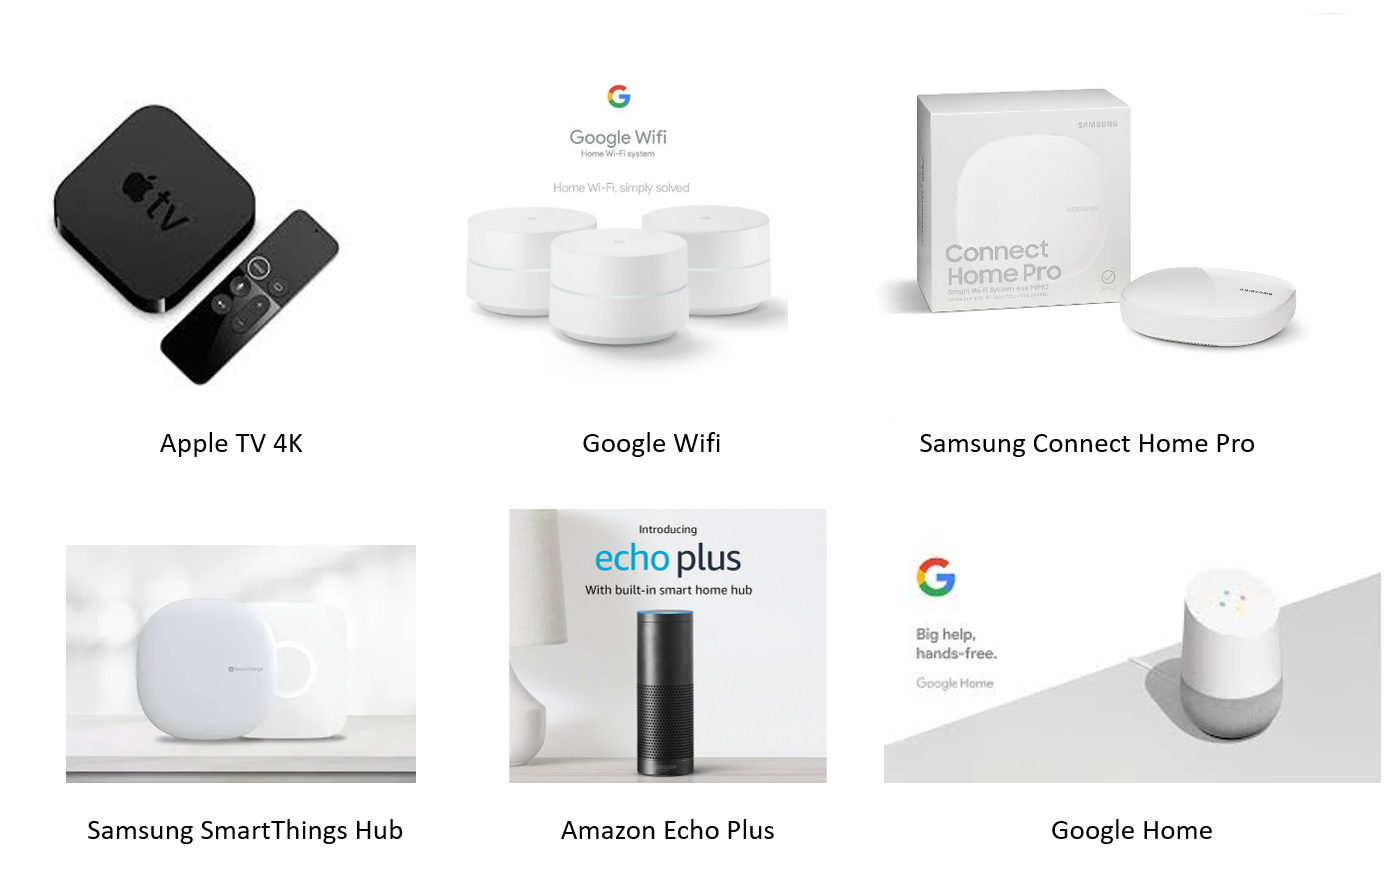
\includegraphics[width=1.0\linewidth]{./Figures/fog_nodes.png}
	\caption[Caption for LOF]{Some existing products that can serve as fog nodes}
	\label{fig: fog nodes}
\end{figure}
Compared with centralised data centres of the cloud, FNs have limited computing power and are distributed, heterogeneous,  and closer to IoT devices~\citep{tordera2016fog}. For instance, Google data centres, which provide services for Google users, are only deployed at 15 locations around the globe\footnote{https://www.google.com/about/datacenters/inside/locations/index.html}, and only two of them are in Asia. In contrast, many FNs would need to be deployed just along a motorway to provide low-latency services for autonomous vehicles (AVs)~\citep{xiao2017vehicular}.  Figure~\ref{fig: fog computing} shows the architecture of IoT and the position of fog computing in this architecture~\citep{bonomi2012fog}. 

% https://www.google.co.uk/imgres?imgurl=https%3A%2F%2Ferpinnews.com%2Fwp-content%2Fuploads%2F2018%2F01%2Fedge-computing-diagram-1024x512.png&imgrefurl=https%3A%2F%2Ferpinnews.com%2Ffog-computing-vs-edge-computing&docid=1ruIYfEWwkRsiM&tbnid=Fq_aYqg8ZYAAcM%3A&vet=10ahUKEwjdlIKVko3cAhXJKsAKHSLCDzMQMwhLKA4wDg..i&w=1024&h=512&bih=836&biw=967&q=fog%20network&ved=0ahUKEwjdlIKVko3cAhXJKsAKHSLCDzMQMwhLKA4wDg&iact=mrc&uact=8
\begin{figure}[!htb]
	\center
	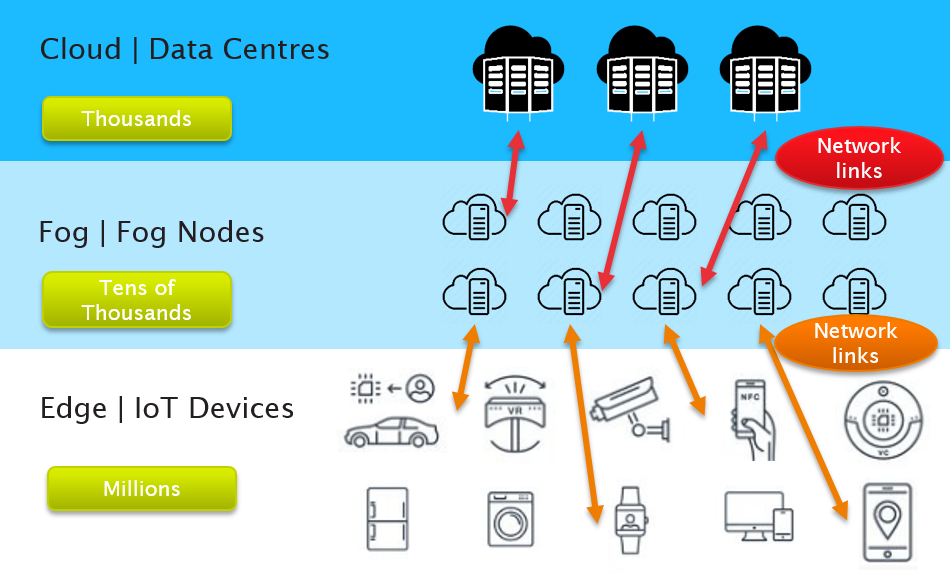
\includegraphics[width=0.9\linewidth]{./Figures/Cisco-fog.png}
	\caption[Caption for LOF]{The architecture of the IoT, fog computing and cloud computing\protect\footnotemark}
	\label{fig: fog computing}
	%   \source{\citep{evans2011internet}}
\end{figure}

\footnotetext{source of icons: https://www.colourbox.com/vector/set-vector-flat-line-icons-internet-of-things-vector-18757991}

Note that there are several computing paradigms that are similar to fog computing, such as geo-distributed clouds~\citep{narayanan2014towards}, edge computing~\citep{garcia2015edge}, mobile cloud computing~\citep{fernando2013mobile} and cloudlets~\citep{satyanarayanan2009case}. Although there are many differences between these computing paradigms, in essence, they all places computational resources close to the users and they all have similar resource allocation models.
%https://arxiv.org/ftp/arxiv/papers/1611/1611.09193.pdf 
As the name suggests, a geo-distributed cloud consists of several geo-distributed cloud data centres, which offer many advantages such as low latency, the ability to safeguard against failures, and exploitation of different regional energy prices. However, compared with fog nodes, the data centres in a geo-distributed cloud is still far away from IoT devices~\citep{narayanan2014towards}. Furthermore, edge computing pushes the computing power directly into the edge of the Internet, that is, applications are processed on IoT devices that have sufficient computing power~\citep{garcia2015edge}, and mobile cloud computing is about offloading computing tasks from mobile devices to computing resource providers such as cloud or fog~\citep{fernando2013mobile}. In addition, cloudlets is just an alternative name for fog~\citep{satyanarayanan2009case}. Given this, in the rest of the report, we refer to fog computing because it is the most appropriate platform for many IoT applications~\citep{bonomi2012fog}, but our discussion and solutions are equally applicable to the other types of systems mentioned.

Similar to the cloud, the primary function of the fog is to provide computing and networking resources, and fog computing is rather a complement to cloud computing than a substitute~\citep{matt2018fog}. The differences between them make fog computing more suitable for many IoT application scenarios. In what follows we highlight important features that fog computing should have~\citep{bonomi2012fog}. Note that, fog computing is recently proposed and have not yet been widely used, and some of these features are shared by both fog and cloud computing.  
% see paper: Integration of Cloud computing and the Internet of Things: A survey

First, the fog should have the ability to execute low latency computational tasks for applications such as AVs, real-time video analytics and online games. For example, at high speed, the response time for the autopilot system of an AV to avoid an accident can be just several milliseconds. Fog computing can reduce latency and network traffic because the data collected by IoT devices will be sent to FNs nearby for processing and storage, instead of sending them to often far-away cloud data centres~\citep{atlam2018fog}.
% Fog services need to satisfy the demands of applications which require low network latency (e.g., autonomous vehicles (AVs), video surveillance, gaming, etc.). Low latency is critical to these applications, for example, if an autonomous vehicle has a high latency, it is more likely to crash because it can drive very fast and emergency may happen at any time. 

Second, since many IoT devices are mobile (e.g., smartphones, laptops, AVs), the fog should support mobility through wireless access. It can use techniques like Locator ID Separation Protocol (LISP)\footnote{http://www.lispmob.org}, Mobile IPv6 (MIPv6) and  Hierarchical Mobile IPv6 (HMIPv6)~\citep{liu2015distributed}. For example, LISP separates the address space of locators and identifiers and has the advantage of mobility. In addition, the mobility of IoT devices brings new challenges to resource allocation such as VM migration and dynamic traffic routing.

Third, the fog also needs to support real-time interactions besides batch processing because real-time interactions are demanded by many IoT applications such as virtual reality (VR) and augmented reality (AR).
% http://delivery.acm.org/10.1145/2350000/2342513/p13-bonomi.pdf?ip=152.78.64.203&id=2342513&acc=PUBLIC&key=BF07A2EE685417C5%2EA13CBF7F1C3C7DF4%2E4D4702B0C3E38B35%2E4D4702B0C3E38B35&__acm__=1530977188_ac059b30da43194f9bf844aee9025c43

Finally, some data of the IoT needs to be processed in the fog and others are more suitable to be processed in the cloud because the cloud has data that the fog does not have or has a greater computing power~\citep{bonomi2012fog}.  As a result, the fog should also support interplay with the cloud, which means that the fog can send data to the cloud to process. For example, the big data generated by a smart grid is first processed in the fog and then the results are sent to the cloud for latency-insensitive analysis~\citep{borylo2016energy}. 

\section{Fog Computing Application Scenarios} \label{application scenarios}

Next, we will introduce the application scenarios that are especially suitable for fog computing, such as AR, VR, real-time video analytics, smart grid and autonomous vehicles. 

\begin{itemize}
	\item \textbf{AR and VR:} AR can ``augment" real-world scenes by adding computer-generated graphics to the real world, and VR constructs an environment of computer-generated feedback of video and sound that makes people have the feeling that the generated world is immersive and realistic. Examples of AR include Microsoft HoloLens~\citep{evans2017evaluating} and Google Glass~\citep{muensterer2014google}, while HTC Vive~\citep{dempsey2016teardown} and Oculus Rift~\citep{desai2014review} are representatives of VR. Since the computer-generated environment should be able to deceive the senses and humans are very sensitive to feedback delays (latencies greater than 50ms are perceptible)~\citep{brooks1999s}, the video must have a high resolution to feel real as well as a high frame rate and very low latency for sensitivity. Consequently, both AR and VR need immense computing power to run properly. However, mobile devices like smartphones often have limited computing power~\citep{yang2018communication}. A possible solution is to combine fog computing and mobile AR or VR devices and put intensive computations in the fog. For example, a startup called GridRaster is developing a VR/AR software platform on Saguna's fog computing solution Open-RAN~\citep{alto2018VR} to offer an immersive VR/AR experience on mobile devices by leveraging fog computing. Furthermore, a large shipbuilder Navantia is starting to use an AR system, which is also based on fog computing. A study of this system shows that fog computing based AR system respond clearly faster than cloud-based AR system~\citep{fernandez2018fog}.
	% file:///C:/Users/fb1n15/OneDrive%20-%20University%20of%20Southampton/PhD/9-month%20report/%E4%B8%AD%E6%96%87%E8%AE%BA%E6%96%87/Fog%20and%20IoT.pdf
	
	\item \textbf{Real-Time Video Analytics:} Real-time video analytics uses artificial intelligence to analyse video contents generated by huge numbers of cameras deployed in buildings, along the streets or in cars in real-time. Fog computing can help many video analytics applications, such as video surveillance, object/face recognition, and smart traffic lights, which typically require low latency, immense computing power and large bandwidth. For example, a bandwidth of 25 Mbps is required to stream a 4K video~\citep{ananthanarayanan2017real}. A prototype of a dynamic urban surveillance system based on fog computing, which uses three drones to monitor vehicles and a laptop as the FN, was built~\citep{chen2016dynamic}. Evaluations showed that this scheme is with great promise for smart urban surveillance applications, as it can track the target all the time in a noisy environment and the estimated speed is close to the actual speed of the target. \citet{ali2018edge} show that the efficiency in the throughput of a facial recognition system using deep learning can be considerably improved by putting initial processing of the data at fog nodes compared to a cloud-only system.
	% Another advantage of fog computing in this scenario is that personal privacies are better protected. (cannot find a ref)
	
	\item \textbf{Smart Grid:} The smart grid is a virtual network which can control the electricity grid including energy load, clean energy and grid safety. Many grid control applications are run on the edge of the network, like smart meters and micro-grids~\citep{wei2014optimally}. As grid networks are distributed widely, it is impractical to offload all computational tasks to the cloud. However, the fog can gather and process data from the grid and do real-time analytics and control. For instance, \citet{singh2018iot} propose and validate an IoT big data analytics system, which uses fog computing, to store, process and analyse energy consumption data from smart homes. In addition, \citet{okay2016fog} propose a three-tier (i.e., smart meters, fog nodes and cloud data centres) smart grid model and show that their model improves the cloud computing based smart grid in terms of privacy, latency, and locality.
	
	\item \textbf{AVs:} An AV is a vehicle that can drive by itself without human interference, which is the trend of the car industry. For example, all Tesla cars have autopilot features such as lane centring, adaptive cruise control, and self-parking~\citep{endsley2017autonomous}, and Google and Apple are also developing their own AVs. An AV uses cameras, radars and other sensors to capture information from the surrounding environment, which must be processed in real time to make proper driving decisions. Since AV applications also need very short latency and high bandwidth to send the data, fog computing is particularly suited to run them~\citep{peter2015fog}. Here, fog nodes can be AVs or static fog nodes such as mart base stations or smart routers. With fog computing, vehicles without sufficient computing power can utilise these fog noes to run compute-intensive applications (e.g., AR driving assistance and VR gaming), and spontaneous exchange of information between AVs is made possible~\citep{xiao2017vehicular}. For example, a two-level architecture (i.e., AVs and fog nodes) is introduced to cope with the challenges of automated driving services such as large content volume, location-dependence and delay-sensitivity~\citep{yuan2018toward}. Another framework called vehicular fog computing, which uses moving vehicles such as taxis and buses as mobile fog nodes, is proposed in order to provide cost-effective and on-demand fog computing service for AVs~\citep{xiao2017vehicular}.
\end{itemize}


% In summary, we believe that fog computing is vital to support in many scenarios of IoT applications.
\section{Fog Computing Resource Allocation} \label{fog computing resource allocation overview}

A typical fog has computing resources in its FNs and networking resources in its network. Computing resources, which generally include processors, random access memory (RAM) and disk storage, are capable of processing computational tasks. Additionally, IoT tasks are processed by virtual machines (VMs) generated in FNs. Here, VMs are emulations of real computers that contain all necessary elements to run fog tasks. Moreover, there are two different types of networking resources. One is the bandwidth among the FNs; the other is the bandwidth between FNs and IoT devices. Specifically, fog systems are owned and operated by fog providers, which can be Internet service providers, wireless carriers, cloud service providers and even fog users who are willing to trade their spare computing resources~\citep{yi2015survey}. Finally, the main business model of fog computing is the pay-per-use business model, i.e., fog users pay for the costs of fog resources when they use it rather than before or afterwards~\citep{yi2015survey}.

The RAFC mainly involves three components, which are task scheduling, VM placement and traffic routing~\citep{gu2018joint}. In detail, task scheduling is deciding when to process each task, and VM placement is assigning VMs, which process fog tasks, to appropriate FNs. Furthermore, traffic routing is finding the paths to send data between IoT devices and FNs. Notably, the latter two components are unique to fog computing and do not apply to centralised cloud computing. 

Against this background, the process of the resource allocation is briefly introduced below~\citep{shi2017online} (Figure~\ref{fig: flow of resource allocation}). First, the fog users report the information about their tasks (e.g., value, demanded resource, processing time and deadline) to the fog provider over time. Then, after receiving the report, the fog provider will immediately decide whether to run the task, how much to charge and how to allocate resource for the task. Finally, the fog provider will send these decisions to the user, process the tasks accordingly and wait for new task requirements. 

\begin{figure} 
	\centering
	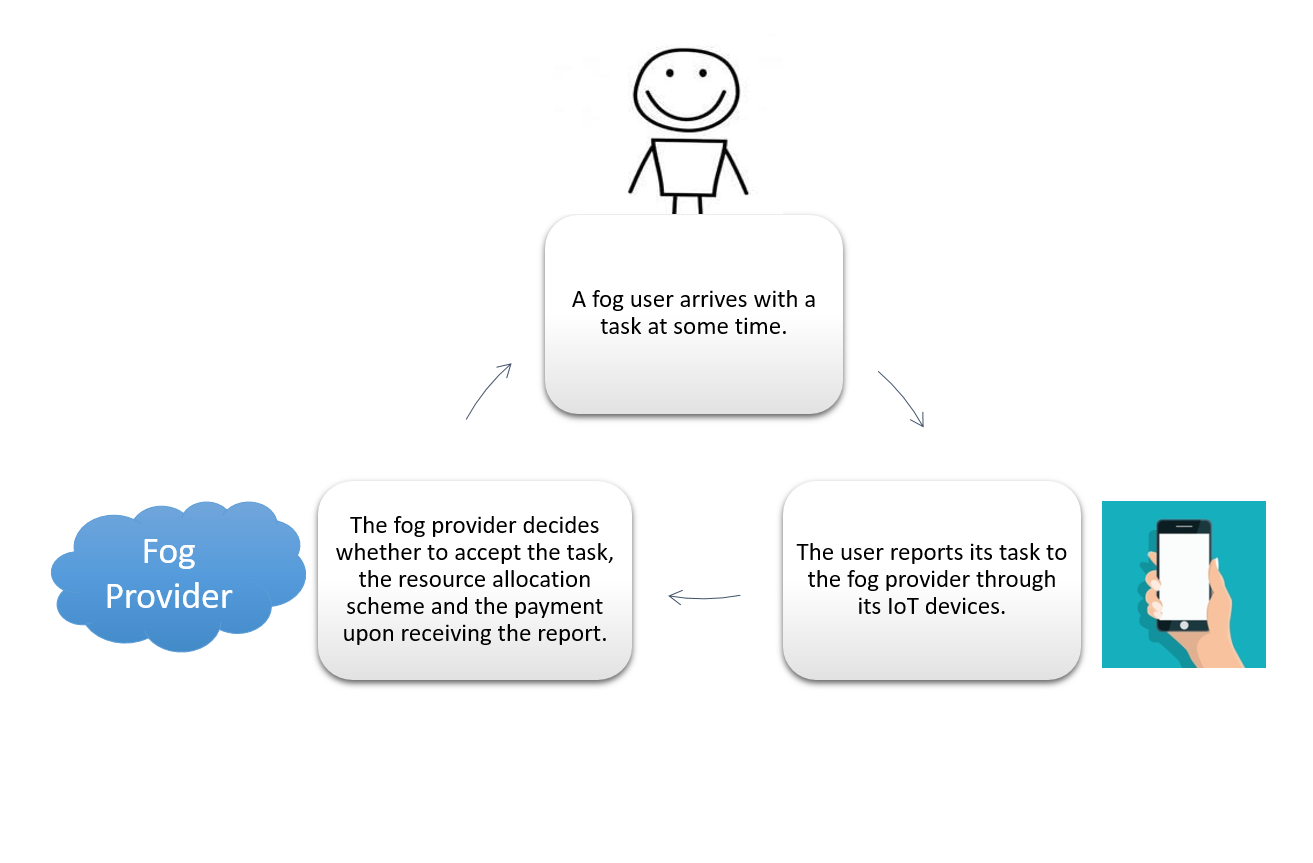
\includegraphics[width=1\textwidth]{./Figures/Allocation_procedure.png}
	\caption{The procedure of fog computing resource allocation\protect\footnotemark}
	\label{fig: flow of resource allocation}
\end{figure}

\footnotetext{source of images: https://www.shutterstock.com/image-vector/hand-holding-smart-phone-vector-illustration-1084761833}

In addition, in a strategic setting, self-interested users can misreport their tasks such as delaying the report, expanding their processing time, declaring a higher value or an earlier deadline for them. In order to prevent misreporting, we can impose regulations and policies and penalise any users who misreport, or we can take the approach of online mechanism design which incentivise fog users to report truthfully. In detail, online mechanism design is a subfield of game theory that studies the problem of how to design mechanisms, which decides allocations of resource and monetary transfers based on received reports, to get desired objectives when rational users arrive over time~\citep{nisan2007algorithmic}. We choose to adopt the approach of online mechanism design to deal with this problem because imposing regulations has been criticised as being costly and slow~\citep{demougin2001monitoring}.

\section{Research Challenges} \label{challenges}

After the introduction of fog computing and the fog computing resource allocation problem, we now discuss the research challenges that we intend to address. 
%see thesis example and add some sentences here

%My main suggestion is, instead of listing the various "resource allocation" challenges, to present your challenges as a set of design requirements that a fog resource allocation mechanism should meet.  

\begin{enumerate}
	
	\item \label{itm: Challenge bandwidth} \textbf{Challenge 1} \textit{Limited bandwidth resources.} If bandwidth in the fog is unlimited and free, it is feasible to just consider allocating computing resources for fog tasks. However, in actual situations, bandwidth is limited and costly. Thus, resource allocation mechanisms in the fog need to take bandwidth into consideration and try to make the best of it to reduce cost or latency. By contrast, bandwidth is usually ignored in cloud computing resource allocation~\citep{shi2016online} because the traffic routing is not controlled by the cloud provider (cloud providers just buy bandwidth from Internet service providers (ISPs))~\citep{kuster2012cloud}. However, the emerging software-defined networking (SDN) (i.e., a network approach that enables the network to be centrally controlled using software)~\citep{kreutz2015software} makes centralised network control in fog computing feasible.
	
	\item \label{itm: Challenge VM} \textbf{Challenge 2} \textit{Dynamic VM allocation.} Another challenge that is unique to fog computing is the dynamic allocation of VMs. Firstly, in our model, VMs are not limited to several types, instead they can be dynamically assembled according to users demands. Secondly, unlike cloud providers, the fog provider needs to choose an FN to generate the VM for newly arrived tasks. Furthermore, in order to keep a low latency to a moving IoT device, the VM may need to be moved from one FN to another every now and then~\citep{bittencourt2015towards}. Beyond that, VMs in the fog also need to move among FNs to serve new tasks efficiently. 
	
	\item \label{itm: Challenge time-oriented} \textbf{Challenge 3} \textit{Time-oriented tasks.} How to allocate time-oriented tasks is another challenge to fog computing. This is because many IoT tasks are time-oriented, which means that they need a certain amount of computational time (between the earlies start time and the deadline of the task) to achieve their maximum value, but they can still achieve part of the value if they are allocated less time. For example, suppose a user wants to run a video surveillance application with facial recognition to surveil their shops for 24 hours. Then, it is still of value to them if the surveillance lasts less than 24 hours, say, 18 hours.
	
	\item \label{itm: Challenge social welfare} \textbf{Challenge 4} \textit{High social welfare resource allocation.} This challenge is about how to maximise the social welfare (i.e., the overall utility) of fog users given the limited computing and networking resources of the fog, especially when there are a lot of users demanding diverse resources dynamically. In more detail, the utility of a computing task represents the value obtained by the fog user from processing that task. Maximising social welfare is a typical mechanism-design goal because social welfare represents the aggregated satisfaction of users.
	
	\item \label{itm: Challenge truthful} \textbf{Challenge 5} \textit{Resource allocation in a strategic setting.} In practice, fog users may be strategic, which means that users can misreport their tasks for their own benefit. In general, such behaviours are detrimental to the overall efficiency of the fog, and possibly lead to much worse system performance than expected. To address this problem, the fog provider may use a truthful resource allocation mechanism. Here, truthfulness (or strategyproofness) means that fog users cannot get a better utility by misreporting their tasks to the fog provider~\citep{nisan2007algorithmic}. This challenge is composed of two parts. The first part is how to design a mechanism that achieves truthfulness while only degrading a little proportion of the efficiency or without a loss compared to the best non-truthful mechanism in a non-strategic setting (i.e., users always report their information truthfully unconditionally). The second part is that this truthful mechanism should also outperform state-of-the-art non-truthful mechanisms in social welfare in a strategic setting.
	
	\item \label{itm: Challenge online} \textbf{Challenge 6} \textit{Resource allocation in online settings.}
	Furthermore, the online nature of the RAFC, which means that allocation decisions have to be made as information of new task reported over time and without any knowledge of the future, makes social welfare maximisation even more challenging. For example, myopic poor decisions can make high-value tasks in the future unable to be schedules, which lead to big losses in social welfare. What's more, it also makes designing truthful mechanisms more challenging. For example, a classical truthful mechanism---VCG mechanism (see Section \ref{mechanism design}) does not work in online scenarios. However, a large amount of literature just focus on offline settings, in which all users report their information simultaneously. 
	
	\item \label{itm: Challenge cost-aware} \textbf{Challenge 7} \textit{Cost-aware resource allocation.} In contrast to most existing literature, which only treat social welfare as the total value of finished tasks, we take resource costs into consideration in our model. Therefore, our problem, which contains a mixture of packing and covering constraints (packing task demands within resource capacities, and covering accepted tasks by paying operational costs of resources)  is more challenging than problems with only packing constraints~\citep{azar2013online}.
	
	\item \label{itm: Challenge scalability} \textbf{Challenge 8}
	\textit{Timely resource allocation.} Since it is common to have ad hoc fog tasks that request to process immediately after the report. The resource allocation mechanism should be computationally efficient so that it can make allocation and pricing decisions right away when it receives new reports of fog tasks. However, the resource allocation problem for fog computing has an NP-hard nature (explained in Section \ref{model of fog}), and the number of fog tasks, fog nodes and IoT devices can be really big. So it is both important and challenging to design very computationally efficient resource allocation mechanisms. 
	
%	Cross-referencing challenge \ref{itm: Challenge cost-aware}
	
	
	%    \item \textbf{Revenue aware resource allocation:} 
	%    % Reducing the cost of the service is always one of the best ways to increase the service provider's revenue. For this reason, how to reduce the cost while giving users adequate levels of service is a crucial challenge for fog providers. In other words, the fog provider needs a resource allocation mechanism that is efficient. 
	%    How to improve fog providers' revenue is another important challenge especially if the fog provider is a for-profit business because the main goal of a for-profit business is to improve its revenue. Furthermore, profitability is also the key to win the fierce market competition.
	
	%    \item \textbf{Computational efficiency aware resource allocation:} In order to provide services which meet expectations of the users, computational efficiency aware resource allocation mechanisms are studied to lower the response time or to boost the execution speed~\citep{younge2010efficient}. The challenge is how to design a computationally efficient mechanism that can allocate resources promptly and reduce the latency of services.
	
	%    \item \textbf{Artificial intelligent resource allocation:} With the fast development of artificial intelligence (AI) techniques, it is promising to use some of them in the resource allocation system to improve performance in social welfare or fog providers' revenue. These techniques include artificial neural network, reinforcement learning and multi-agent systems. In particular, AI resource allocation is especially useful in a dynamic environment because it can predict computing tasks and their resource demands~\citep{sembiring2013dynamic}.
	
	%merged into AI resource allocation
	%\item \textbf{Dynamic resource allocation:} The demands of fog users often fluctuate a lot over time or geographically. It is critical to retain a high quality of service (QoS) of fog computing, which means the levels of availability, reliability and performance offered by cloud providers~\citep{Ardagna2014}, under such fluctuation of demand while keeping the cost of the system as low as possible. 
	%
	%\item \textbf{Predicted resource allocation:} Predicting the users' demands and reserving resources for future tasks can significantly improve the efficiency of the fog~\citep{patel2015aggregation}. The challenge is how to predict the fog computing demand precisely, fast and cheaply.
	
	
	
	
\end{enumerate}

% There are also some other interesting research challenges. Although we did not address them in our existing work, they can be the domains for our future work. For example: 

% \begin{enumerate}
% \item \textbf{Load balancing aware resource allocation:} The main aim of load balancing is to avoid overload of any of the FNs and to optimise the performance of the whole fog computing system~\citep{aslam2015load}. As a result, the fog services can satisfy more users even when their demands or locations varies a lot over time.

% \item \textbf{Power aware resource allocation:} The energy consumed by data centres could account for 20\% of all electricity by 2025 if no significant improvement is made about the efficiency of it~\citep{Power}. This is definitely unfavourable to the environment and the global climate change. By reducing the heat generated and the power consumption of the FNs, the fog provider can also lower the cost and obtain an advantageous position in the fierce market competition. For example,~\citep{ali2016energy} proposed an energy efficient algorithm by placing virtual machines on most energy-efficient physical machines first. 

% \item \textbf{QoS aware resource allocation:} This challenge focuses on the QoS of the fog provider. The wide geographical distribution of the fog makes it more challenging to guarantee the QoS than the cloud.

% \item \textbf{Resource allocation for mobile endpoints:} The placement of resources such as computing power and bandwidth for the mobile endpoints may vary over time. This imposes a significant challenge to the resource allocation system of the fog. For example, if an autonomous vehicle is driving on the road, the FN that processes its data needs to keep changing so that the latency of the service meets the SLA. A placement and migration method is proposed in~\citep{ottenwalder2013migcep} to deal with this challenge. By planning the migration ahead of time, this method keeps the latency low while reducing the bandwidth required to do the service migration. 
% \end{enumerate}


\section{Research Contributions} \label{contributions}

%in the contributions you *have* to refer to these requirements (or challenges, whatever you have). 
In order to address the research challenges listed above, this report takes the approaches of constrained optimisation and online mechanism design to study the problem of RAFC with the aim of maximising social welfare. In more detail, constrained optimisation is a domain in mathematical optimisation whose goal is to find the values of related variables to optimise an objective function given some constraints of these variables~\citep{bertsekas2014constrained}. In our problem, the objective function, which is to be maximised, calculates the total social welfare, and constraints consist of both resource constraints and time constraints. Furthermore, we take the approach of online mechanism design because we intend to design a truthful online mechanism and in our problem users arrive over time and thus resource allocation decisions must be made online.

The main contribution of this report is proposing a truthful mechanism that can also achieve near-optimal social welfare of fog users. By designing, implementing and evaluating our resource allocation mechanism, we show that it achieves better social welfare than benchmarks and achieves social welfare close to the optimal (around 90\%) in a strategic setting. Specifically, we make the following three contributions to address the challenges in Section~\ref{challenges}.

\begin{enumerate}
	\item \textbf{We formulate the fog computing resource allocation problem as a constraint optimisation problem.} In order to address challenges \ref{itm: Challenge bandwidth}--\ref{itm: Challenge time-oriented} mentioned above, we formulate the fog computing resource allocation problem, which considers the bandwidth constraints and traffic routing as well as allows flexible allocation of VMs, as a constraint optimisation problem. We also model it as an online mechanism design problem where a fog task requests an amount of processing time with specific resource demands.
	
	%\textbf{Study and implement benchmark mechanisms:} An offline optimal algorithm is implemented to compute the theoretical upper bound of the social welfare performance. In addition, an online greedy algorithm and a variant of the Social Welfare Maximization Online Auction (SWMOA) algorithm~\citep{shi2017online} are implemented as the benchmarks of online truthful mechanisms. 
	
	\item \textbf{We design a truthful mechanism and evaluate its performance in social welfare.} We design a new truthful and individually rational (IR) mechanism called flexible online greedy (FlexOG). A mechanism is called IR if no participants can get a negative utility by participation~\citep{nisan2007algorithmic}. Thus, under our mechanism, fog users will truthfully report their tasks as soon as they get them. By extensive simulations, we show that FlexOG achieves social welfare better than that achieved by the state-of-the-art benchmarks (up to 10\%) and is close to the optimal value (around 90\%). Therefore, we have addressed challenge \ref{itm: Challenge social welfare},\ref{itm: Challenge online},\ref{itm: Challenge cost-aware} and part one of challenge \ref{itm: Challenge truthful}, which is designing a truthful mechanism that outperforms state-of-the-art truthful mechanisms.
	
	\item \textbf{We conduct simulations to show that our truthful mechanism performs better than online optimal, which is a non-truthful mechanism, in a strategic setting.} To fully address challenge \ref{itm: Challenge truthful}, we show that FlexOG achieves better social welfare than the online optimal mechanism, which optimally allocates resources over time with the information it has received, in a strategic setting by simulations. This is surprising because online optimal achieves a better social welfare if all users report truthfully. We choose online optimal as the benchmark here because online optimal is a greedy algorithm, which is good enough for resource allocation under uncertainty~\citep{gupta2017stochastic}. First, we show that on average, non-truthful users have a higher utility than truthful users under the online optimal mechanism, so that fog users indeed have incentives to misreport their tasks. Then, we show that when even a small proportion of users misreport, the social welfare achieved by online optimal declines significantly and is lower than that achieved by FlexOG. This is interesting because in literature Price of Anarchy (PoA) (i.e., the ratio between the optimal centralised solution and the worst Nash equilibrium\footnote{In a Nash equilibrium, no user can benefit by changing their strategy unilaterally.}) is often studied to measure how the efficiency (e.g., social welfare, revenue, and average latency) of a system degrade when its users are self-interested and rational~\citep{koutsoupias1999worst}. Another way to measure this is using the price of sinking, which is the biggest ratio between the value of the optimal solution and the value of a sink equilibrium (i.e., an equilibrium repeated selfish behaviours converge)~\citep{goemans2005sink}. However, PoA cannot apply to our model because often pure strategy Nash equilibria do not exist and randomised strategies are unrealistic in our case. Furthermore, the price of sinking is also not suitable here because in our model fog users are not fixed, and they do not always acquire fog services repeatedly. So we study how a truthful mechanism actually performs compared with a non-truthful one in a strategic setting by simulations.
\end{enumerate}


\section{Outline of the Report} \label{outline}
This report consists of five chapters. Specifically, in Chapter~\ref{literature review} we outline the literature which is related to our research and the techniques they use to address the challenges listed in Section~\ref{challenges}. It includes the related theory of game theory and mechanism design (Section~\ref{preliminaries}) and the related resource allocation mechanisms proposed for MARA (Section~\ref{general multiagent resource allocation}), RACC (Section~\ref{cloud computing resource allocation}) and RAFC (Section~\ref{fog computing resource allocation}). In Chapter~\ref{our mechanism} and Chapter~\ref{simulation and results}, we demonstrate the contributions of our research, including our model of RAFC (Section~\ref{model of fog}), the descriptions and properties of benchmarks and our proposed mechanism (Section~\ref{benchmarks} and Section~\ref{FlexOG}), the experimental setup for simulations (Section~\ref{experimental setup}) and results and analysis of the simulations (Section~\ref{results and analysis}). Finally, we draw conclusions from the research so far and detail our planned future work in Chapter~\ref{conclusions and future work}


\chapter{Literature Review} \label{literature review}

%Similarly, in the related work, you need to refer back to the challenges and say why they don't address them.
Since the main aim of our work is to design a truthful mechanism that is efficient in terms of social welfare as described in the previous chapter. In this chapter, we provide the necessary background for our research and relevant literature on resource allocation mechanisms for non-strategic settings and truthful resource allocation mechanisms for strategic settings. Our main aim is to explore the progress of current research, their advantages and disadvantages and evaluate the extent to which the research challenges in Section \ref{challenges} have already been addressed and what research gaps are still left open.

We begin our literature review with the relevant knowledge in algorithmic game theory (Section \ref{preliminaries}) including the pertinent concepts of game theory, mechanism design and online mechanism design because it is the theory of designing mechanisms that achieve a specific outcome including truthfulness (Challenge \ref{itm: Challenge truthful}). Then in Sections \ref{general multiagent resource allocation}, \ref{cloud computing resource allocation} and \ref{fog computing resource allocation}, we examine the work on general multiagent resource allocation (MARA), resource allocation in cloud computing (RACC) and resource allocation in fog computing (RAFC) respectively, and discuss what challenges they address and what challenges are still open. Finally, Section \ref{literature review summary} summarises our findings and the main research gaps according to our research challenges.

\section{Preliminaries} \label{preliminaries}
Given that mechanism design is the theory we use to deal with the problem of resource allocation in strategic settings (Challenge \ref{itm: Challenge truthful}), in what follows we explain the main concepts before proceeding to related work. If the reader is familier with the basics of game theory and mechanism design, they can choose to skip this section. Mechanism design is a domain in game theory (i.e., the study of participants' strategies and behaviours in a certain game, which means a formal model of an interactive situation). It studies how to design the mechanism, which makes decisions of resource allocation and money transfer, of a game to achieve certain desirable properties or outcomes under the assumption that all participants are rational~\citep{hurwicz1973design}. 

Traditionally, game theory and mechanism design are widely used in the field of microeconomics as important analysis tools. Furthermore, they are also used in some computer science problems such as sponsored search auctions~\citep{zhu2012truthful}, spectrum auctions~\citep{qin2015sponsored} and bandwidth allocation~\citep{wu2012auction}. Particularly, online mechanism design is an extension of mechanism design which deals with problems in a dynamic environment (Challenge \ref{itm: Challenge online}) where agents are allowed to come and go at any time, such as the smart grid, cloud computing or fog computing. In contrast, classic mechanism design only deals with static environments. For example, in a spectrum auction, telecommunications suppliers submit their bids before the deadline and the spectrum allocation decisions are made all at once. Similarly, in sponsored search auctions, once someone searches online, the advertisers bid for advertisement slots simultaneously, and then a decision is made to decide how all the slots will be assigned. 

The structure of this section is as follows. 
In Section \ref{game theory}, we introduce the basic concepts of game theory. In Section \ref{mechanism design}, we examine the relevant concepts and theorems of mechanism design and show a representative example. Finally, we introduce online mechanism design and discuss some results in a special online domain called single-valued online domain in Section \ref{online mechanism design}

\subsection{Game Theory} \label{game theory}

Game theory is ``the study of mathematical models of conflict and cooperation between intelligent rational decision-makers"~\citep{roger1991game}. In more details, in game theory, decision makers are often called agents, players or participants, and we use the term agents in this thesis. To analyse agents' behaviours, we must make assumptions about how they behave. In game theory, this assumption is that all agents are rational, which means they always strive to maximise their utility. The utility of an agent is the quantification of its preference over all outcomes of a game, that is, a real number is assigned to each outcome, and this is defined as its utility. If the utility of outcome $ a $ is greater than that of outcome $ b $ for the agent, then it prefers outcome $ a $ to outcome $ b $. In the game, every agent tries to get the best outcome for itself and also knows that other agents similarly try to achieve the best outcomes for themselves. In order to achieve this goal, agents follow strategies that decide their behaviours in all situations. Researchers in game theory have applied these mathematical models to understand decision making in economics~\citep{gu2005price,kelly2003decision}, biology~\citep{hammerstein1994game,dugatkin2000game} and multi-agent systems~\citep{parsons2002game,semsar2009multi}. Furthermore, RAFC can be modeled as a game, where fog users are players of the game, and they act to compete for fog resources (see the details in Section \ref{model of fog}).
In game theory, a simultaneous game (e.g., rock-paper-scissors) is a game where each agent chooses its actions without any knowledge of the actions of other agents. Our RAFC problem belongs to this type of game because fog users are assumed to not have any information of other users' actions, although they do not take actions at the same time. First of all, we present a rigorous mathematical definition of a simultaneous game, so that we can introduce other concepts based on it.
Formally, we define a simultaneous game as consisting of a finite set $I$ of agents, $I = \{1,2,...,n \}$. The relevent traits of agent $ i $ (e.g., preferences and time constraints ) are summarised as the type $ \theta_i \in \Theta_{i} $ of that agent, and the type profile $ \theta = \{ \theta_1, \theta_2, \ldots, \theta_n\} $ is the set of all agents' types. The behaviour of agent $ i $ is captured by a function that maps from all its possible types to its set of actions: $\Theta_i \rightarrow X_i$, which is called the strategy of agent $ i $. $S_i$ is the set of all strategies of agent $i$. The strategy of agent $i$ and the strategies vector of other agents are $s_i$ and $s_{-i}$, respectively. Then the vector of strategies selected by all agents is $s=(s_1,s_2...,s_n)$. The set of all possible vectors of strategies is denoted as $S$, and the set of all possible vectors of strategies except agent $i$'s is $S_{-i}$. The utility of agent $i$ when it plays strategy $s_i$ and others play strategy $s_{-i}$ is $u_i(s_i,s_{-i}) \in \mathbb{R}$. 
% the difference between utility and valuation function

In addition, the strategies of agents can be categorised into pure strategies and mixed strategies. A pure strategy uniquely determines the behaviour of an agent for any situation (the state of the game) it can face. In other words, an agent using a pure strategy will always take the same action when it faces the same situation. On the other hand, a mixed strategy is an assignment of a probability to each pure strategy. This allows an agent to randomly choose a pure strategy when it needs to take actions. In this thesis, we focus on pure strategies because we aim to incentivise agents to use a pure strategy, which is to truthfully reveal their types.
%There are many game types under different assumptions and with their own corresponding analogues in real life. For example, they can be divided into cooperative/non-cooperative games according to whether agents can cooperate through external enforcement. They can also be divided into simultaneous/sequential games according to whether agents take actions simultaneously or not. Moreover, they can be divided into perfect information/imperfect information games according to whether all the information is known by every agent. 

%Then, we introduce the pure strategy game, which is a classical model in perfect information game and is what we try to design in this thesis. In a pure strategy game, every agent can only use one strategy from its strategy set. ;

%\subsubsection{Solution Concepts} \label{solution concepts}

Furthermore, given a game, there are different ways to predict its result. We use solution concepts to describe how we predict game results, and these predictions are called solutions. There are two basic solution concepts needed in this thesis: dominant strategy equilibrium and Nash equilibrium. Here, an equilibrium means a strategy profile (i.e., a set of strategies for all players) which is stable enough to be predicted as the actual result of the game. 

To present dominant strategy equilibrium, we first introduce dominant strategies of agents. If an agent has a unique best strategy in the game regardless of other agents' choices, then we call it a dominant strategy for that agent. Namely, $s_i^* \in S_i$ is the dominant strategy for agent $i$, if: \[u_i(s_i^*,s_{-i}) > u_i(s_i,s_{-i}),\quad  \forall s_i \neq s_i^* ,\,  s_{-i} \in S_{-i}.\]
%Then, the dominant strategy equilibrium is the set of all dominant strategies (i.e., $s^*=(s_1^*,s_2^*,...,s_n^*)$).
Furthermore, a weakly dominant strategy for agent $i$ is a strategy such that no other strategies are better than it. Formally, $s_i^* \in S_i$ is a weakly dominant strategy for agent $i$, if: 
\[u_i(s_i^*,s_{-i}) \geq u_i(s_i,s_{-i}),\quad \forall s_i \neq s_i^* ,\,  s_{-i} \in S_{-i}.\] 

Then, a strategy vector $ s \in S $ is called a dominant strategy equilibrium, if every strategy in it is a weakly dominant strategy:
\[u_i(s_i,s_{-i}') \geq u_i(s_i',s_{-i}'),\quad \forall  i \in I ,\, s_i' \in S_i,\, s_{-i}' \in S_{-i}\] 
%Similarly, the set of all weakly dominant strategies $s^*=(s_1^*,s_2^*,...,s_n^*)$ is called a weakly dominant strategy equilibrium. 
It is important to note that if a game has a dominant strategy equilibrium, each agent has a best strategy regardless of other agents' strategies. This property is very useful when we design mechanisms because if the dominant strategy equilibrium of a mechanism is desirable, this mechanism can be used in strategic settings and still get this desirable equilibrium. For example, if we hope that the strategy of every agent is simply to reveal its type truthfully, then the corresponding equilibrium is desirable in this case. Thus, it is the most widely used solution concept in mechanism design, and we focus on designing mechanisms that have dominant strategy equilibria in this thesis. 

%
However, in most games, there is no dominant strategy equilibrium, because in these games, an agent's best strategy changes with other agents' strategies. The stable equilibria in these games are called Nash equilibrium, which is one of the most important concepts in game theory and has widespread applications. In a Nash equilibrium, no agent can benefit from changing its behaviour unilaterally. Formally, a strategy vector $ s\in S $ is called a Nash equilibrium if:
\[u_i(s_i,s_{-i}) \geq u_i(s_i',s_{-i}),\quad \forall  i \in I ,\,  s_i' \in S_i.\] 
Nash equilibria can exist in a stable manner because no agent in the Nash equilibrium has an incentive to change its strategy. So normally games will end up in one of its Nash equilibria if it has one. This solution concept is not very convincing in predicting agents' strategies if there is more than one Nash equilibrium in a game~\citep{nisan2007algorithmic}. Furthermore, the Nash equilibria are not guaranteed to be reached even when it is unique because an agent's belief of other agents' strategies may be incorrect. 

% \subsection{Bayesian Game}
% When the agents in the game do not have complete information but only have beliefs of other agents, we call these games Bayesian games. They are called Bayesian games because agents in these games can update their belief of others using Bayes' rule as the game goes on. The Bayesian game can be defined as: $G = <N, <{\Theta}_i, S_i, p_i, u_i>_{i \in N} >$, where $N$ is the set of all agents; $S_i$ is the set of strategies of agent $i$; ${\Theta}_i$ is the set of possible types of agent $i$; $p_i$ is the probability distribution over ${\Theta}_i$ for agent $i$; $u_i : {\Theta} \times S \rightarrow R$ is the utility function for agent $i$. 

% We assume that agents are risk neutral and only try to maximise their expected utilities. Then the Bayesian Nash equilibrium means that each type of agent chooses a strategy that maximises its expected utility given the actions of other type agents and its beliefs about other agents' types. Namely given a Bayesian game $G = <N, <{\Theta}_i, S_i, p_i, u_i>_{i \in N} >$, if there exists a strategy vector $s^*=(s_1*,s_2*,...,s_n*)$ such that: $u_{{\theta}_i}(s_{{\theta}_i}*, s_{-{\theta}_i}*) \geq u_{{\theta}_i}(s_{{\theta}_i}, s_{-{\theta}_i}*), \quad \forall s_{{\theta}_i}\in S_i,\; \forall i \in N, \; \forall {\theta}_i \in {\Theta}_i,$ then it is called a Bayesian Nash equilibrium. This equilibrium is a very useful tool to analyse dynamic games of incomplete information. 

\subsection{Mechanism Design} \label{mechanism design}

We now introduce the core concept of this thesis–mechanism design, which can be viewed as reverse game theory. For game theory, the goal is to analyse the strategies and behaviours of agents in a certain game (as described in Section~\ref{game theory}), while for mechanism design, the goal is to design the mechanism of the game to achieve a certain result or social choice (i.e., an aggregation of different types of agents toward a single collective decision) in a strategic setting~\citep{nisan2007algorithmic}. Since the types (or part of the types) of the agents are usually private (i.e., not common knowledge), mechanism design is necessary under these circumstances. In particular, the designer of the mechanism does not participate in the game. Instead, it designs the mechanism, or rules of the game, to achieve certain goals (e.g., social welfare maximisation or revenue maximisation). Since the mechanism designer needs to make decisions based on agents' types, the difficulty of mechanism design is how to incentivise agents to reveal their true types. 

In order to model strategic behaviours of the agents, a model called independent private values, and strict incomplete information game~\citep[Chapter 9]{nisan2007algorithmic} is adopted in this thesis. Independent private values mean that the valuation of an agent is not affected by any other agents' information. Here, the valuation function of an agent represents its valuation of the result it gets. Unlike the utility function, this does not include any payments (see Definition \ref{general mechanism}). 
Strict incomplete information means that there is no probabilistic information in the model. For example, we do not know the distribution of valuation functions. This model is reasonable in our RAFC scenario, in which users are assumed to have independent valuation functions and have no knowledge about the types of others, and the mechanism designer has no probabilistic information about the agents either (Challenge \ref{itm: Challenge truthful}). Here, a game comprises a mechanism environment and a mechanism. We first introduce the mechanism environment.

\begin{definition}[mechanism environment]
	A mechanism environment \sloppy $ \mathcal{E} = (I, A, \{X_i\}_{i \in I}, \{\Theta_{i}\}_{i \in I}, \{v_i\}_{i \in I}) $ contains the following ingredients:
	\begin{enumerate}
		\item A set of $n$ agents: $I$
		\item A set of results: $ A $
		\item For every agent $i$, a set of actions $X_i$
		\item For every agent $i$, a set of possible types $\Theta_i$. The type of agent $i$ is $\theta_i \in \Theta_i$
		\item For every agent $i$, a valuation function $v_i:\Theta_i \times X_1 \times \cdots \times X_n \rightarrow \mathbb{R}$, which maps from the type of agent $i$ ($ \theta_i $) and the actions taken by all agents ($ x_1,x_2,\ldots, x_n $) to a real number~\citep[Definition 9.40]{nisan2007algorithmic}
	\end{enumerate}
\end{definition}

In the following sections, we introduce some foundamental concepts and theories in mechanism design. Specifically, we introduce the definitions of social choice function and mechanism (Section \ref{social choices and mechanisms}), and we describe a special type of mechanisms called direct-revelation mechanisms along with an important theory called the revelation principle (Section \ref{direct-revelation mechanisms and truthfulness}).
%From the above definition, we can see that each agent needs to choose an action without knowledge of other agents' types or actions. In mechanism design, we design mechanisms (see Definition below) to make the strategies of agents desirable.
% In particular, we wish that the game induced by the mechanism have a desired dominant strategy solution so that the strategies of agents are incentivised to that desired by us. 
\subsubsection{Social Choices and Mechanisms} \label{social choices and mechanisms}

Building on the general definitions, we next introduce the notion of a general (nondirect-revelation) mechanism. A general mechanism is composed of two components: an outcome function that chooses a result based on the profile of agents' actions, and a payment functionthat decide a payment for every agent also based on the profile of actions.
% We consider mechanisms with money (Challenge \ref{itm: Challenge cost-aware}) in this thesis because this is common practice in resource allocation like smart grid, cloud computing and fog computing. 
% Formally, the set of alternative results is $A$. The preference of a agent $i$ is quantified by a valuation function $v_i : A \rightarrow \mathbb{R}$. An agent's utility $u_i$ is the difference between its value $v_i$ and payment $p_i$.

\begin{definition} [mechanism]\label{general mechanism}
	A general mechanism $ \mathcal{M} = (a, \{p_i\}_{i \in I}) $ comprises:
	\begin{enumerate}
		\item an outcome function $a : X_1 \times \cdots \times X_n \rightarrow A $
          %        outcome function actions -> A, social choice function types -> A ?
          \item payment functions $p_1,\ldots,p_n$, where $p_i : X_1 \times \cdots \times X_n \rightarrow \mathbb{R}$
          \citep[Definition 9.24]{nisan2007algorithmic}.
      \end{enumerate}
  \end{definition}

  Then, the game induced by a mechanism over some mechanism environment is formally defined below.
  \begin{definition}[games of mechanisms]
      The game $ \Gamma(\mathcal{M}) $ induced by a mechanism $ \mathcal{M} = (a, \{p_i\}_{i \in I}) $ over mechanism environment $ \mathcal{E} = (I, A, \{X_i\}_{i \in I}, \{\Theta_{i}\}_{i \in I}, \{v_i\}_{i \in I}) $ is the strict incomplete information game $ \Gamma(\mathcal{M}) = (I, \{\Theta_{i}\}_{i \in I}, \{X_i\}_{i \in I}, \{u_i\}_{i \in I}) $ where the agents' utility functions $u_i(\theta_i,x_1,\ldots,x_n) = v_i(\theta_i,a(x_1,\ldots,x_n)) - p_i(x_1,\ldots,x_n)$
	\citep[Definition 9.24]{nisan2007algorithmic}.
\end{definition}

\begin{definition}[social choice function]
  The social choice function $f$ maps the types of agents to the results (allocation of goods):
	$$f : \Theta_1 \times \cdots \times \Theta_n \rightarrow A$$ 
  \label{social choice function}
\end{definition}

In general, we want to design a mechanism that can get the same outcome of a desired social choice function (e.g., a social choice function that maximise the total utilities of the agents). So if the equilibrium under a mechanism maps to the same result as a social choice function, we say that this mechanism implements this social choice function.

\begin{definition}[implementation]
	The mechanism implements a social choice function $f : \Theta_1 \times \cdots \times \Theta_n \rightarrow A$ in dominant strategies if for some dominant strategy equilibrium $s_1,\ldots,s_n$ of the induced game, where $s_i: \Theta_i \rightarrow X_i$ we have that
	$$ f(\theta_1,\ldots,\theta_n) = a(s_1(\theta_1),\ldots,s_n(\theta_n)), \quad \forall \theta_1,\ldots,\theta_n \in \Theta $$
	\citep[Definition 9.24]{nisan2007algorithmic}.
\end{definition}

In the following section, we introduce a special type of mechanism called direct-revelation mechanisms and a property of mechanisms called truthfulness. Then we introduce the revelation principle, which shows that we can just focus on direct-revelation truthful mechanisms when designing mechanisms.

\subsubsection{Direct-Revelation Mechanisms and Truthfulness} \label{direct-revelation mechanisms and truthfulness}
There is a special type of mechanism called a direct-revelation mechanism, which is very important in mechanism design because of the revelation principle (see Proposition \ref{revelation principle}). In a direct-revelation mechanism, the set of actions of agent $i$, $X_i$, is the set of its possible types $ \Theta_i $, which means what an agent can do is just to reveal its type to the mechanism.  To formally introduce this definition below, we first introduce some notation. We denote the set of all possible valuation functions for agent $i$ as $V_i$, and the vector of all types except agent $i$'s as $\theta_{-i} = (\theta_1,\ldots,\theta_{i-1},\theta_{i+1},\ldots,\theta_n)$. Similarly, we define $\Theta_{-i} = \Theta_1 \times \cdots \times \Theta_{i-1} \times \Theta_{i+1} \times \cdots \times \Theta_n$.
%Similarly, $V = V_1 \times \cdots \times V_n$ and $V_{-i} = V_1 \times \cdots \times V_{i-1} \times V_{i+1} \times \cdots \times V_n$. 

\begin{definition} [direct-revelation mechanisms]
	A direct-revelation mechanism $(f,p_1,...,p_n)$ is composed of a social choice function $f$ and a vector of payment function $(p_1,...,p_n)$.
	The payment functions $(p_1,...,p_n)$ maps the reported types of agents to the payments of agents, where
	$$p_i : \Theta_1 \times \cdots \times \Theta_n \rightarrow \mathbb{R}$$
	\citep[Definition 9.14]{nisan2007algorithmic}.
\end{definition}

Now we introduce the definition of truthfulness, which is a key concept in this thesis. It is also called strategy-proofness or dominant-strategy incentive-compatibility (DSIC). Under a truthful mechanism, agent $i$ would prefer providing its true type to the mechanism regardless of other agents' strategies, because by providing false information agent $i$ cannot increase its utility. In other words, truthful mechanisms can prevent agents from misreporting and manipulating.

\begin{definition}[truthfulness]
	A mechanism $(f,p_1,...,p_n)$ is called truthful or DSIC  if $v_i(f(\theta_i, \theta_{-i})) - p_i(\theta_i, \theta_{-i}) \geq v_i(f(\theta_i', \theta_{-i})) - p_i(\theta_i',  \theta_{-i}), \quad \forall \theta_i , \theta_i' \in \Theta_i ,\, \theta_{-i} \in \Theta_{-i} $~\citep[Definition 9.15]{nisan2007algorithmic}.
\end{definition}


%In particular, a social choice function combines the types of agents to reach a collective decision on the choice of candidates:
%
%\begin{definition}
%    A function $f: \Theta_1 \times \cdots \times \Theta_n \rightarrow A$ is called a \textit{social choice function}.
%    \citep[Definition 9.1]{nisan2007algorithmic}.
%\end{definition}
We can now introduce a fundamental principle in mechanism design called the revelation principle. It is fundamental because this principle shows that it is sufficient to just study direct-revelation truthful mechanisms to find out if it is possible to implement social choice function $f$ in dominant strategies. This principle makes mechanism design much easier by narrowing the space of mechanisms that need to be searched. 

\begin{proposition}(Revelation principle) \label{revelation principle}
	Any social choice functions $f$ that can be implemented in dominant strategies by a general mechanism can also be implemented by a direct-revelation truthful mechanism. Moreover, the payments of the agents in the truthful mechanism are the same as those in the equilibrium of the original mechanism~\citep[Proposition 9.25]{nisan2007algorithmic}.
\end{proposition}


%While indirect-revelation mechanisms are all the types of mechanisms except for direct-revelation mechanisms. 

In the following, we introduce two desirable properties of a mechanism besides truthfulness in this thesis. The first desirable property is called individual rationality (IR), which guarantees that all (rational) agents are willing to participate. This is required because agents in our RAFC problem cannot be forced to participate in the mechanism. To satisfy this property, the mechanism should guarantee that no agents will get negative utility by joining the game. 
\begin{definition} [IR]
	A mechanism is individually rational if no agent gets negative utility by participating the game (i.e., $v_i(f(\theta_1,...,\theta_n)) - p_i(\theta_1,...,\theta_n) \geq 0, \quad \forall \theta_1 ,\ldots,\theta_n \in \Theta_n, \, i \in I$)~\citep[Definition 9.18]{nisan2007algorithmic}
\end{definition}

%The second desired property is no positive transfers, which means the payment from any agent to the mechanism is not negative. A mechanism which has positive transfers is difficult to maintain itself, thus often not practical to use in real life.
%\begin{definition}
%    A mechanism has no positive transfers if the payments from agents are never negative. Namely, we have $p_i(v_1,...,v_n) \geq 0, \quad \forall v_1 \in V_1,\ldots,v_n \in V_n,\; \forall i \in N$~\citep[Definition 9.18]{nisan2007algorithmic}
%\end{definition}

The second desired property is weak budget balance (WBB), which means that the total payment from agents is not lower than the overall cost. Here, the cost function $ o: f(\theta_1,...,\theta_n) \rightarrow \mathbb{R} $ of the mechanism maps from resource allocation decisions to the overall operational cost of the resource (Challenge \ref{itm: Challenge cost-aware}). This property is desired because normally fog providers try to avoid losses. So they are not willing to adopt a mechanism that is not WBB. 

\begin{definition}
	A mechanism is weakly budget balanced if it will never run a deficit. Formally if for every $ \theta_1,\ldots, \theta_n $ we have that $ \sum_{i \in I} p_i(\theta_1,...,\theta_n) \geq \sum_{i \in I} o(f(\theta_1,...,\theta_n)) $. 
\end{definition}


To design truthful mechanisms, we define important properties of truthful mechanisms in the following. These properties can be used to help design mechanisms or judge if a mechanism is truthful. 
\begin{proposition}
	A mechanism is truthful if and only if it satisfies the following conditions $\forall i \in I,\; \theta_{-i} \in \Theta_{-i}$:
	\begin{enumerate}
		\item The payment $p_i$ only depends on the outcome of the game $f(\theta_i, \theta_{-i})$, namely, for every $\theta_{-i}$, there exist prices $p_a \in \mathbb{R}, \; \forall a \in A$, such that for all $\theta_i$ with $f(\theta_i, \theta_{-i})=a$ we have that $p_i(\theta_i,\theta_{-i}) = p_a$
		\item The mechanism optimises for each agent (i.e., $f(\theta_i, \theta_{-i}) \in argmax_a(v_i(a) - p_a), \quad \forall \theta_i \in \Theta_{i}$)~\citep[Proposition 9.27]{nisan2007algorithmic}. 
	\end{enumerate}
\end{proposition}

Then, the following definition describes the property a social choice function must have in a truthful mechanism. This property is called weak monotonicity (WMON), and it means that if the result changes when an agent changes its valuation function, then the agent's value of the new result relative to its value of the old result should also be increased.
\begin{definition}
	A social choice function $f$ satisfies Weak Monotonicity if $ f(\theta_i, \theta_{-i}) = a \neq b = f(\theta_i', \theta_{-i}) \implies v_i(a) - v_i(b) \geq v_i'(a) - v_i'(b) \quad \forall i \in I, \;  \theta_i,\theta_{i}' \in \Theta_i, \; \theta_{-i} \in \Theta_{-i} $~\citep[Definition 9.28]{nisan2007algorithmic}.
\end{definition}

Then, the following theorem means that WMON is a necessary condition for truthfulness but becomes a sufficient condition only if all domains of types are convex sets. More specifically, a convex set is a set of points, for every pair of points within it, every point on the straight line that joins them also lies within the set.

\begin{theorem}
	If a mechanism $(f,p_1,...,p_n)$ is truthful, $f$ satisfies Weak Monotonicity (WMON). In addition, for every WMON $f$ there exists payment function $p_1,...,p_n$ such that the mechanism $(f,p_1,...,p_n)$ is truthful only if all domains of types $\Theta_i$ are convex sets~\citep[Theorem 9.29]{nisan2007algorithmic}.
\end{theorem}


\subsection{Online Mechanism Design} \label{online mechanism design}

In this section, we extend the framework of classic mechanism design to online mechanism design, which deals with time-dynamic scenarios where agents' types are reported over time and decisions must be made without future information. So unlike an offline mechanism, which just makes one overall decision, an online mechanism must make a sequence of decisions over time. 
%Furthermore, besides agents' reports, stochastic events could also happen over time, and we use $ \omega \in \Omega $ to denote the set of possible stochastic events. 
Many real-world scenarios are dynamic, such as allocating computational resources to tasks being submitted over time, allocating electrical power to electric cars arriving over time or selling seats on an aeroplane to passengers. 
The RAFC problem we study in this thesis is also dynamic because fog users report their tasks over time and allocation decisions must be made at the same time of reports.

Online mechanism design faces challenges that are different from (offline) mechanism design because the environment is dynamic~\citep[Chapter 16]{nisan2007algorithmic}. In particular:
\begin{enumerate}
	\item Decisions must be made without future information.
	\item Other than their valuation functions, agents can also misreport their private information about time, such as the arrival times and deadlines of their tasks (Challenge \ref{itm: Challenge time-oriented})
	\item (limited misreports) In practice, an agent may not be able to misreport their type without limitations. For example, in the RAFC scenario, it is impossible to report a task before the agent knows it needs to run this task. So an agent can only misreport a later arrival time of its task.
\end{enumerate}

Next, we discuss the component of a dynamic environment in this thesis. $T = \{ 1,2,\ldots,t \}$ denotes discrete (possibly infinite) time steps. Let $q = (q^1,q^2,\ldots)$ denote the sequence of decisions (e.g., accepting/rejecting an agent, the payment of an agent, and when to serve an agent) which can be made when receiving reports from agents. The type of agent $ i $, $\theta_i = (T_i^a,T_i^d,v_i) \in \Theta$, where $T_i^a,T_i^d \in T$ are its arrival time and departure time (deadline), and $ v_i(k) \in \mathbb{R} $ is its valuation function. On the other hand, the reported type of agent $ i $ is denoted as $\hat{\theta}_i = (\hat{T}_i^a,\hat{T}_i^d,\hat{v}_i) \in \Theta$, which may be different from $ \theta_{i} $ because agents can misreport in our setting. The mechanism state $h^t = (\theta^1,\ldots, \theta^t; q^1,\ldots,q^{t-1}) \in H^t$ denotes the mechanism state in time step $ t $, where $ H^t $ is the set of possible mechanism states in time step $ t $. It contains the information of agent types ($\theta^1,\ldots, \theta^t$), and decisions ($q^1,\ldots,q^{t-1}$) that have been made. Furthermore, we use $ Q(h^t) $ to denote all possible decisions in state $ h^t $. ~\citep[Section 16.2]{nisan2007algorithmic}

In the following section, we extend the direct-revelation mechanisms and revelation principle to the online domain. Furthermore, we give formal definition of limited misreports and the definition of truthfulness under limited misreports. 

\subsubsection{Direct-Revelation Online Mechanisms} \label{direct-revelation online mechanisms}


Now we are ready to introduce the definition of a direct-revelation online mechanism. A direct-revelation online mechanism is an extension of a direct-revelation offline mechanism, but it has more restrictions on agents' behaviours. Note that the mechanism we design for RAFC in Section~\ref{FlexOG} belongs to this type of mechanism because the only actions fog users can take are to report their types and they report over time. 

\begin{definition}[direct-revelation online mechanism]
	In a direct-revelation online mechanism, each agent only sends a single report about its type to the mechanism. The mechanism consists a social choice policy $f =\{f^t\}^{t\in T}$ and a payment policy $p = \{p^t\}^{t\in T}$, where decision $ f^t(h^t) \in Q(h^t) $ is made in mechanism state $ h^t $ and payment $ p_i^t(h^t) $ is the money that agent $ i $ needs to pay to the mechanism. For convenience, we denote the sequence of decisions as $f(\theta) = (q^1,q^2,\ldots)$ and overall payment collected from agent $i$ as $p_i(\theta) \in \mathbb{R}$, given type profile $ \theta $~\citep[Definition 16.2]{nisan2007algorithmic}.
\end{definition}

%\subsubsection{Limited Misreports} \label{limited misreports}
Unlike offline scenarios, in certain online scenarios, it is reasonable to assume some limitations on the domain of the misreports, which can also simplify the mechanism design problem. For example, agent $ i $ cannot report an earlier arrival time than its true arrival time ($ \hat{T}_i^a < T_i^a $) or report a later deadline ($ \hat{T}_i^d > T_i^d$). This is a very natural assumption because agent $ i $ has no idea of its type before its true arrival time $ T_i^a $, and reporting a later deadline will make the task miss its deadline. 

\begin{definition}[limited misreports]
	The limited misreports that an agent can make is denoted as $C(\theta_i) \subseteq \Theta_i$, where $\theta_i$ is the type of agent $i$~\citep[Definition 16.4]{nisan2007algorithmic}.
\end{definition}

%It is also important to note that in this thesis, we focus on one types of truthful mechanism: dominant-strategy incentive-compatible (DSIC) mechanisms:
%% and Bayes-Nash incentive-compatible (BNIC) mechanisms. The latter is a weak solution which requires more assumptions. In BNIC mechanisms, truthful revelation is the best strategy in expectation only when other agents also use this strategy.   
%

Then, we introduce the definition of a truthful online mechanism given limited misreports, which is similar to the definition of a truthful (offline) mechanism.

\begin{definition}[truthful]
	Given limited misreports C, a truthful or DSIC online mechanism satisfies:
	\[ v_i(\theta_i,f(\theta_i,\theta_{-i})) - p_i(\theta_i,\theta_{-i}) \geq v_i(\theta_i,f(\hat{\theta_i},\theta_{-i},\omega)) - p_i(\hat{\theta_i},\theta_{-i}), \]
	\[ \forall \hat{\theta_i} \in C(\theta_i), \, \theta_i \in \Theta_i, \;  \theta_{-i} \in \Theta_{-i} \]
	\citep[Definition 16.5]{nisan2007algorithmic}.
\end{definition}

% \begin{definition}(BNIC)
% Given limited misreports C, a Bayes-Nash incentive-compatible (BNIC) online mechanism satisfies:
% \[ \mathbb{E} \{ v_i(\theta_i,\pi(\theta_i,\theta_{-i},\omega)) - p_i(\theta_i,\theta_{-i},\omega) \} \geq \mathbb{E} \{  v_i(\theta_i,\pi(\hat{\theta_i},\theta_{-i}',\omega)) - p_i(\hat{\theta_i},\theta_{-i}',\omega) \}, \]
% \[ \forall \hat{\theta_i} \in C(\theta_i), \forall \theta_i \in \Theta_i, \]
% where the expectation is with respect to the distribution on other agents' types $\theta_{-i}$, random events $\omega$, and randomisations in the policy $\pi$.
%~\citep[Definition 16.6]{nisan2007algorithmic}.
% \end{definition}

%% need to make this principle clear
Unfortunately, unlike (offline) mechanism design, only studying direct-revelation truthful online mechanism is not without loss of generality because the online revelation principle does not always hold. However, if the agents are assumed to have no-early arrivals ($ \hat{T}_i^a \geq T_i^a $) and no-late departures ($ \hat{T}_i^d \leq T_i^d $), then the online revelation principle still holds. Alternatively, revelation principle can be recovered by demanding each agent to send a non-informative ``heartbeat'' message in every time step $ t \in [\hat{T}_i^a, \hat{T}_i^d ] $ besides the report of its type~\citep[Section 16.22]{nisan2007algorithmic}. In our RAFC model, although fog users can report late departures, it is reasonable to ask them to send a ``heartbeat'' message in every time step. So we focus on truthful direct-revelation online mechanisms in our work. 

In the following sections, we examine related work on MARA (Section \ref{general-multiagent-resource-allocation}), RACC (Section \ref{resource-allocation-in-cloud-computing}), and RAFC (Section \ref{resource-allocation-in-fog-computing}). Specifically, RAFC is the domain we study in this thesis, RACC is a close domain with many similarities, and MARA is the big domain that RAFC and RACC belongs to. We analyse the different resource allocation models they deal with, the techniques they use, and why their approach cannot directly apply to our RAFC problem.

\section{General Multiagent Resource Allocation} \label{general-multiagent-resource-allocation}
In this Section, we discuss recent work on general MARA, in which resources are distributed among several agents and these agents may have an impact on the allocation results ~\citep{chevaleyre2006issues}. MARA is relevant to a wide range of applications such as resource allocation in electricity grids~\citep{gradwell2005distributed}, network routing~\citep{feldmann2003selfish}, RACC~\citep{wang2017multiagent} and RAFC~\citep{yi2015survey}, which is the problem we focus on in the thesis. 

\subsection{Background} \label{multiagent resource allocation}

Formally, MARA models the following resource allocation problems. There is a set of resources $ Z $ and a set of agents $ I $. The resources may be indivisible or divisible (e.g., electricity, RAM and storage). Similar to what is described in Section~\ref{direct-revelation mechanisms and truthfulness}, agents report their preferences over the bundles of resources (i.e., collections of resources that wrapped together) by means of utility functions
(i.e., functions that assign a real number (utility) to each bundle to represent the  agents' preferences) 
The goal is to find the resource allocation plan that maximises the social welfare.

Now, there are different types of social welfare, some common ones are utilitarian, egalitarian, and Nash product social welfare. Utilitarian social welfare is the most common one, which is the total sum of the utilities achieved by all agents, and it is also the social welfare we try to maximise in this thesis (Challenge \ref{itm: Challenge social welfare}). In some cases, egalitarian social welfare, which measures the lowest utility of any agent, is more appropriate. For example, in a disaster rescue problem, it is more important to reduce casualties than to improve the total utility of the victims~\citep{roos2010complexity}. Furthermore, Nash product social welfare, which is the product of agent' utilities, is a synthesised indicator of both total utility and fairness~\citep{moulin2004fair}. Here, fairness means that the difference between different agents' utilities is small. 
%An important issue in MARA is the representation of utility function because different representation can lead to different computational complexity of finding the optimal allocation. The most straightforward method to represent utility is called bundle enumeration. Namely, all bundles of resources are enumerated, and each bundle is given a utility. Even though bundle enumeration is fully expressive, its usually impractical because the representation gets from this method is exponential in the number of resources. Another method to represent utility is called k-additive form, which defines the utility of agent $ i $ for bundle $ B \subseteq R $ of resources by
%\[ u_i^k(B) = \sum_{T\subseteq B, \, \|T\| \leq k} \alpha_i^T, \]
%where $ \alpha_i^T $  is a coefficient for each bundle $ T\subseteq B $ with $ \|T\| \leq k $. The advantage of the k-additive form is that it is expressive when k is large and compact when k is small~\citep{rothe2015economics}. Note that it is also fully expressive when k is large enough.

%\todo[inline]{find out the difference between divisible and indivisible goods}
In terms of utility functions of MARA problem, some properties (e.g., monotonicity, submodularity, subadditivity, and fractional subadditivity) are usually assumed to hold because they are realistic for many applications~\citep{nisan2000bidding}. In the following, we give a formal definition of these properties. Let $ u: 2^Z \rightarrow \mathbb{R} $ be a utility function.
\begin{itemize}
	\item $ u $ is monotonic if $ u(X) \leq u(Y)$ $ \forall$ $ X, Y $ with $X \subseteq Y \subseteq Z $.
	\item $ u $ is submodular if $ \forall$ $ X, Y $ with $X \subseteq Y \subseteq Z $ and $ \forall x \in Z \char`\\ Y $ we have that $ u(X \cup \{x\}) - u(X) \geq u(Y \cup \{x\}) - u(Y) $.
	\item $ u $ is subadditive if $ \forall X,Y \subseteq{Z} $ we have that $ u(X \cup Y) \leq u(X) +u(Y) $.
	
	\item $ u $ is a fractionally-subaddtive function if there exists a collection of set functions, $ \{a_1,a_2,\ldots,a_l\}  $ such that each $ a_j $ is additive (i.e., the value of $ X \subseteq Z $ is the sum of the values of the items in X), and $ u(X) = \max_{j=1}^la_j(X) $.
\end{itemize}
In our problem, the utility function of agents satisfies three properties of them, except for submodularity (see Section \ref{model of fog}). This is reasonable for our model, because often the processing time near the accomplishment of a fog task is much more valuable than the previous processing time, which causes the utility function to not be submodular.

%In terms of their relationship, every submodular utility function is fractionally subadditive, and every fractionally subadditive utility function is subadditive~\citep{nisan2000bidding}.

Furthermore, resource allocation mechanisms can generally be categorised into two main classes, namely, centralised mechanisms and distributed mechanisms. For centralised mechanisms, there is a central authority in charge of allocating the resources to the agents, based on the utility functions of the agents. A typical example is a combinatorial auction, where bidders bid for bundles of resources and the auctioneer is the central authority. However, centralised mechanisms have the following disadvantages: they require communication between agents and the central authority to always be stable and reliable; the optimal allocation is often computationally hard; the procedure is not very flexible due to its centralised nature~\citep{friedlander1982decentralized}.  To address these disadvantages, many fully or partially distributed allocation mechanisms~\citep{herreiner2002simple,bouveret2011general} are proposed. Under a fully distributed mechanism, agents execute the mechanism totally by themselves, while under a partially distributed mechanism, agents execute the mechanism with the help of a central authority. However, distributed allocation mechanisms cannot guarantee the optimality of the allocation results in most situations~\citep{rothe2015economics}. What's more, to design a truthful distributed mechanism that works in a strategic setting is challenging~\citep{feigenbaum2004distributed}. Thus, we concentrate on centralised mechanisms in this thesis, although centralised or distributed mechanisms can both be used in RAFC.


\subsection{Offline Mechanisms for General Multiagent Resource Allocation}

In this section, we mainly look at a typical offline centralised mechanism for MARA called combinatorial auctions. In a combinatorial auction, agents can bid on combinations (bundles) of discrete items, rather than individual items or continuous quantities. The main challenge of combinatorial auctions is the winner determination problem (WDP), which is how to optimally allocate resources because it is hard to compute (this problem is NP-complete in the general case~\citep{sandholm2002winner}). Now, algorithms to solve the WDP can be categorised into two classes, namely, exact methods and approximate methods. For exact methods, the optimal allocation is guaranteed to be found given enough computation time. In contrast, approximate methods cannot guarantee the optimality of their solutions, but they usually take less time to solve the WDP and have better scalability.

In terms of exact methods, branch-and-bound (BB) based algorithms~\citep{sandholm2002winner,sandholm2002algorithm} are classic methods to solve the WDP with hundreds of items. Furthermore, branch-on-bids (BoB)~\citep{sandholm2003bob}, branch-on-items (BoI)~\citep{sandholm2000improved}, and combinatorial auction BoB (CABoB)~\citep{sandholm2005cabob} algorithms are proposed to solve the WDP of similar scale faster.
% To reduce the processing time, \citet{fujishima1999taming} introduce the combinatorial auction structural search (CASS), which try to avoid considering allocations that contain conflicting bids. In addition, for more complex problem in which each item can have multiple units, and each bid can specify bundles with unrestricted units of each item, \citet{leyton2000algorithm} extend CASS to combinatorial auctions multi-unit search (CAMUS), which is a novel algorithm based on BB and uses techniques such as removing dominated bids, dynamic programming and heuristics. 
Moreover, some traditional approaches are also used to solving the WDP, for example, integer programming~\citep{andersson2000integer}, constraint programming~\citep{porter1999effect}, and dynamic programming~\citep{rothkopf1998computationally}. However, the above algorithms work well only with a small number of items, and their time and space complexity can be high for large combinatorial auction problems.

In order to solve WDPs faster or solve large WDPs, many approximate methods are proposed, which are usually based on heuristics or meta-heuristics. Some famous examples of these are: greedy algorithms~\citep{krysta2005greedy}, stochastic local search (SLS)~\citep{boughaci2010local}, genetic algorithms~\citep{boughaci2009memetic}, simulated annealing~\citep{guo2006heuristics}, Casanova~\citep{hoos2000solving}, memetic algorithms~\citep{boughaci2009memetic} and ant colony optimisation~\citep{ray2018ant}. 
%The memetic algorithm, which combines intensification and diversification of search, has been shown to outperform GA, SAGII and Casanova~\citep{boughaci2009memetic}. Furthermore, ant colony optimisation has been shown to performs significantly better than memetic algorithm on large instances of WDPs~\citep{ray2018ant}. 
However, approximate methods cannot guarantee the optimality of the results.

Overall, the above mechanisms only work for combinatorial auctions, which are about allocating indivisible items in offline scenarios and non-strategic settings. Thus, they only address our Challenge \ref{itm: Challenge social welfare} and do not deal with online scenarios (Challenge \ref{itm: Challenge online}) or strategic settings (Challenge \ref{itm: Challenge truthful}).

In order to address Challenge \ref{itm: Challenge truthful}, considerable work has been done on designing truthful mechanisms for combinatorial auctions. Although the classic VCG mechanism (outlined in Section \ref{VCG machanisms}) is truthful and can achieve optimal social welfare, it is usually computationally hard and infeasible to implement in practice. For this reason, most proposed mechanisms try to achieve a better approximation ratio in polynomial running time. Here, the approximation ratio of a mechanism is the ratio between the optimal social welfare and the result obtained by the mechanism. Let $ |Z| = z $ denotes the number of items, then, \citet{dobzinski2005approximation} propose an $\mathcal{O}(\sqrt{z})$-approximation mechanism for submodular valuations under the most restrictive assumptions. Furthermore, a series of papers improve the approximation ratio from $\mathcal{O}(\log^2{z})$ for fractionally subadditive valuations~\citep{dobzinski2006truthful}, to $\mathcal{O}(\log{z}\log{\log{z}})$ for subadditive valuations~\citep{dobzinski2007two}, to $ \mathcal{O}(\log{z}) $ for submodular valuations~\citep{krysta2012online}, and eventually to $ \mathcal{O}(\sqrt{\log{z}}) $ for fractionally subadditive valuations~\citep{dobzinski2016breaking}. However, these approaches do not apply to online scenarios (Challenge \ref{itm: Challenge online}).


\subsection{Online Mechanisms for General Multiagent Resource Allocation}

Now, we discuss some work on truthful online mechanisms for MARA, which addresses our Challenges \ref{itm: Challenge social welfare}, \ref{itm: Challenge truthful} and \ref{itm: Challenge online}. In particular, we mainly look at resource allocation in EV charging because this problem is similar to RAFC and some work in this field also inspires the techniques used in our work. For example, the users all arrive over time requiring some resource and have deadlines for this resource. However, there are also many differences between them such as an EV can charge the grid while IoT devices cannot send the resource back to the fog and the resource in the grid is homogeneous while the resources in the fog are heterogeneous. However, the work we discuss in this section does not proactively address the dynamic VM allocation challenge (Challenge \ref{itm: Challenge VM}) and the limited bandwidth challenge (Challenge \ref{itm: Challenge bandwidth}). 

%First, a method is introduced to transform a mechanism for online MARA into a truthful one in a discrete time system and single-valued preference domains~\citep{parkes2007ironing}. The method is called ``ironing'' because it achieves truthfulness by cancelling allocation decisions that violate monotonicity. However, the main drawback of this method is that it is often computationally difficult because it needs to consider all possible misreports from users. 

First, model-free mechanisms are adopted by a large part of the literature. Here, model-free mechanisms are those mechanisms that do not predict the demand and supply of resources in the future. The advantages of model-free mechanisms are that they need fewer assumptions and are usually easier to compute. Although these mechanisms are myopic, their efficiency of resource allocation can be near-optimal in certain scenarios. For example,
\citet{gerding2011online} consider the problem of hybrid electric vehicles charging. Since hybrid vehicles can use both electricity and petrol, they have marginal non-increasing valuations for the electricity charged and have no lower limit of the power charged. To make the mechanism truthful, they combined a greedy algorithm with a technique called ``burning" which leaves some units of electricity unallocated when there is still demand unsatisfied. The timing of the ``burning" can be at the allocation of the resource or the departure of the users. In simulations, this mechanism's performance is close to a non-truthful scheduling algorithm and much better than a fixed price mechanism. However, the ``burning" technique may reduce the efficiency of the mechanism significantly. To deal with the hybrid electric vehicle charging problem with various charging speeds, \citet{robu2011online} present two greedy-algorithm-based online mechanisms that incentivise users to truthfully report not only their valuations for the electricity but also their maximum charging rate. The ``burning" technique is also used in this literature to achieve truthfulness. Furthermore, a two-sided pricing mechanism, in which both the EV drivers and charging stations report their private information is presented~\citep{gerding2013two}. However, this mechanism is only truthful for EV drivers. Additionally, \citet{nejad2017online} proposed a framework for EV charging which takes incentives of both the EV drivers and charging stations in a preemption aware setting and a class of model-free mechanisms called MOSAP-X which are fast and near-optimal. 

Furthermore, model-based mechanisms, which consider possible future arrivals, are used by some work to improve the performance of the mechanisms (Challenge \ref{itm: Challenge social welfare}).  \citet{stein2012model} studied the problem of pure electric vehicles charging and proposed a model-based truthful online mechanism to allocate electricity. The mechanism modified the consensus algorithm~\citep{bent2004value} by a technique called pre-commitment to achieve truthfulness. 
In the consensus algorithm, some future scenarios are sampled, and then the scheduling is solved for every one of them. Then, these scenarios vote to decide whether to accept a job (in their case, an EV charging job) or not. 
A mechanism with pre-commitment will only commit to an agent that the requested resource will be allocated before its departure, but when and how the resource will be allocated remains flexible. Real data simulations showed that this mechanism significantly outperforms a model-free algorithm and is nearly as efficient as an offline optimal algorithm. Moreover, \citet{strohle2014online} considered the scenario where both the supply and demand for electricity are uncertain. They also developed a truthful online mechanism based on the consensus algorithm, which achieves near-optimal efficiency. 
%Apart from only charging electric vehicles (EVs), using EVs as electricity storage is considered by \citet{gerding2016online}. Two truthful heuristic online mechanisms are proposed to schedule both the charge and discharge of EVs in car parks. They also have shown that a car park can still make a profit using these mechanisms even though they do not ask for payment from EVs. 

%{Can discuss this approach of designing mechanisms.}

Most of the above literature finds truthful resource allocation mechanisms by looking for an allocation policy that satisfies WMON and then coupling it with a critical-value payment function. However, some literature takes the approach of price-based mechanisms which decide the resource price before allocation. For instance, \citet{hayakawa2015online} presented a class of price-based truthful online mechanisms which can be used in scenarios where electricity has various marginal generation costs, and users have multi-dimensional preferences by using carefully designed pricing functions and scheduling algorithms. They showed that their mechanism has near optimal efficiency in a realistic setting with different marginal costs. Moreover, they also present a class of price-based mechanisms allowing increasing marginal valuations, which is DSIC and IR in settings with uncertain procurement costs, multi-unit demand and multi-minded bidders (Challenge \ref{itm: Challenge time-oriented})~\citep{hayakawa2018price}. 
% Then, they propose three mechanisms belonging to this class of mechanisms. The first is called the first-come-first-served (FCFS) mechanism, which allocates optimally for each newly arrived agent while keeping existing allocation fixed. The payment of each agent is the corresponding (maximum or expected) marginal costs. If the mechanism uses the maximum cost, it is called FCFS(Max). Otherwise, it is called FCFS(Est). The second mechanism is called count all agents (Count), whose pricing function calculates the total number of units that can be allocated. The last one is to pay externality of the virtual market (PayEX), whose pricing function for agent $ i $ is
%based on a virtual market of all other agents without $ i $. In terms of WBB, FCFS(Max) is ex-post WBB, FCFS(Est) is ex-interim WBB, Count is ex-post WBB (if its parameters are set to certain numbers), but PayEx does not guarantee ex-interim WBB. Through numerical evaluations, they demonstrated that in terms of social welfare, FCFS perform well if the prediction of future cost is accurate or resource supply is very tight,
%while PayEX has good performance when future costs are very uncertain, and supply is sufficient. 
Although their system model is similar to ours (see Section \ref{our mechanism}) and our work is based on this class of mechanisms, they only assume homogeneous resource. Specifically, they do not consider limited bandwidth resource (Challenge \ref{itm: Challenge bandwidth}) or deal with the dynamical assembly of VMs from several different types of resource (Challenge \ref{itm: Challenge VM}). Therefore, their resource allocation framework has been adapted for our RAFC problem in this thesis.

\section{Resource Allocation in Cloud Computing} \label{resource-allocation-in-cloud-computing}
% https://ieeexplore.ieee.org/stamp/stamp.jsp?tp=&arnumber=7582511
In this Section, we examine work on RACC, because RACC and RAFC have many similarities. We mainly focus on the Infrastructure-as-a-Service (IaaS) clouds in this section because the service model of fog computing in this thesis is IaaS (see Section \ref{model of fog}). Here, IaaS is a service model that serve users by directly providing computer infrastructures. More specifically, cloud providers pack computational resources (e.g., CPU, RAM and storage) into VMs and provide these VMs to their users. Now, most IaaS cloud providers typically offer pre-configured VM instances of fixed types instead of dynamic VM instances with arbitrary VM configurations (Challenge \ref{itm: Challenge VM}). For example, Amazon EC2 currently offers five categories and 24 types of VMs, and each type has one or more instance sizes\footnote{https://aws.amazon.com/ec2/instance-types/}. In terms of resource allocation mechanisms, most cloud providers, such as Amazon Web Services (AWS)\footnote{https://aws.amazon.com/}, Microsoft Azure\footnote{https://azure.microsoft.com/en-gb/}, and Google Cloud\footnote{https://cloud.google.com/} provide long-term reservation plans or short-range on-demand fixed-price plans to their users. However, long-term reservation plans are obviously not suitable for users with uncertain tasks, which is common in IoT scenarios.  Although fixed-price mechanisms are easy to implement and are obviously truthful, they are not very efficient in social welfare (Challenge \ref{itm: Challenge social welfare}) or revenue mainly because fixed-price mechanisms fail to discriminate different types of tasks~\citep{al2013cloud}. For example, a high-value task would not get a high priority in a fixed-price mechanism. Furthermore, they also fail to cater to the volatility of the market, which leads to underpricing or overpricing. To improve efficiency in revenue, spot pricing is also adopted by these cloud providers such as
Amazon EC2\footnote{https://aws.amazon.com/ec2/spot/pricing/}, Azure Low-Priority VM\footnote{https://azure.microsoft.com/en-gb/blog/low-priority-scale-sets/}, and Google Preemptible VM Instances\footnote{https://cloud.google.com/compute/docs/instances/preemptible}. With spot pricing, a cloud user bids a price for its task, the task will run when the spot price is lower than its price, and the user pays the spot price. However, this mechanism has no guarantee of SLA. Specifically, the spot price is volatile, and thus tasks can be interrupted frequently, and there is no guarantee of the finish time of the task. In addition, the spot pricing mechanism is not truthful (Challenge \ref{itm: Challenge truthful}) either~\citep{wang2012cloud}.

\subsection{Offline Mechanism for RACC}

To date, many truthful mechanisms are designed for RACC in an offline setting. Some work designs truthful mechanisms for static VM provisioning, where the cloud provider has several types of resources and various kinds of VMs, and the cloud users request bundles of VMs with valuations~\citep{wang2012cloud,zaman2011combinatorial,nejad2015truthful}. \citet{zaman2011combinatorial} design a truthful auction for dynamic VM allocation (Challenge \ref{itm: Challenge VM}), which is based on an approximation algorithm. However, they only show the performance of their mechanism by simulations, but without giving a theoretical guarantee. \citet{wang2012cloud,nejad2015truthful} propose truthful VM allocation mechanisms, which combine greedy allocation algorithms and carefully designed payment functions, to get near-optimal allocations. In addition, \citet{zhang2014dynamic,shi2014online} design truthful mechanisms using linear programming (LP) decomposition techniques (i.e., breaking the LP up into smaller problems and solving them separately) for dynamic VM allocation (Challenge \ref{itm: Challenge VM}). \citet{mashayekhy2015ptas} also look at heterogeneous resources allocation in cloud computing, and their proposed mechanism proved to be a polynomial-time approximation scheme, that is, their mechanism can get a solution that is within a factor $ (1-\epsilon) $ of being optimal, where $ \epsilon $ denotes the approximation error. However, the running time of their mechanism still can be exponential in $ 1/ \epsilon $. For tasks with deadlines, a truthful allocation and pricing mechanism and a general framework for transforming allocation mechanisms into truthful ones in a domain of single-minded agents are proposed by~\citet{jain2015near} to maximise social welfare. They also extend their mechanism to maximise revenue for cloud providers and show that its performance is comparable to that of an ideal fixed-price mechanism. Although these mechanisms address our Challenges \ref{itm: Challenge social welfare} and \ref{itm: Challenge truthful}, they fail to address our Challenge \ref{itm: Challenge online}, which is critical to our problem.

\subsection{Online Mechanism for RACC}
To further address Challenge \ref{itm: Challenge online}, there has been a lot of work on designing mechanisms for RACC in an online manner. For example, \citet{wang2013revenue,zhang2016framework} propose online auctions for RACC, but they only consider VM instances of a single type and neglect the dynamic allocation of different VMs (Challenge \ref{itm: Challenge VM}). Moreover, a posted pricing mechanism is proposed by \citet{zhang2017optimal}, under which the cloud provider publishes dynamic unit prices for different resource types, and cloud users either accept the current rates or give up running their jobs. A threshold-based mechanism is also proposed by \citet{farooq2018adaptive} to maximise the revenue of the cloud provider. In their model, the cloud provider has a limited number of VMs with different computational efficiency, and tasks with different complexity that arrive over time. However, these mechanisms do not work in a strategic setting (Challenge \ref{itm: Challenge truthful}). 

%  Furthermore, \citet{zhang2018online} propose a truthful heuristic mechanism for a model, where VMs are flexible, and users can submit multiple requirements, but the cloud provider will at most accept one requirement. 
Therefore, there is a growing body of work looking at how to efficiently allocate cloud resources to users in an online and strategic setting, and many truthful mechanisms have been proposed in recent years. The early mechanisms only apply to very simple settings. For example, \citet{wang2012pcloud,zhang2016framework} propose truthful mechanisms in the setting of single type VMs, and \citet{lin2010dynamic} treat cloud computing resources as homogeneous. However, this is quite impractical because cloud providers usually have more than one type of VM and more than one type of resource (Challenge \ref{itm: Challenge VM}).

For this reason, dynamic virtual machine allocation where cloud providers can decide how to generate the type and number of VMs is also studied by some researchers. For example, \citet{shi2014rsmoa} look at the setting of multi-type VMs and multi-type users. They use a non-decreasing pricing curve to decide the allocation of the resources and the payments of users and claim that their truthful mechanism RSMOA is both efficient in the social welfare of the system and the revenue of the cloud provider. Additionally, an online combinatorial auction framework for dynamic resource allocation in cloud computing is proposed by \citet{shi2014online}. This framework is able to model dynamic allocations of heterogeneous virtual machines and optimise system social welfare over a period of time. Primal-dual optimisation is used to transform a centralised approximation algorithm to a truthful auction mechanism. They showed that this auction framework is also computationally efficient, truthful and has a guaranteed competitive ratio. Here, the competitive ratio is the worst ratio between the social welfare incurred by an online mechanism and the optimal social welfare. However, their work does not study the temporal correlation in decision making, owing to the fact that tasks can span several time slots (Challenge \ref{itm: Challenge time-oriented}). 

Furthermore, some researchers also studied truthful resource allocation mechanisms for tasks with deadlines (e.g., financial companies need data analysis results before the next market open time). For instance, \citet{lucier2013efficient} propose two deadline-aware algorithms for homogeneous resource (i.e., CPU time) allocation in two settings. In one setting, the tasks can be paused and resumed (preemptible), but in the other setting, once a task is started, it must be processed until completion. They design a mechanism using the dual fitting technique for the first setting and prove its competitive ratio as well as show that it significantly outperforms other heuristics used in practice. For the other setting, they prove that no performance guarantee can be given, and propose an efficient heuristic called \textsc{Committed} for resource allocation. Finally, they prove that their \textsc{Committed} algorithm can be made truthful very easily.
Additionally, preemptive scheduling with the assumption of deadline slackness (i.e., the lower bound on the ratio between the requested time of a task and the time window in which it can be processed) has also been studied~\citep{azar2015truthful}. A truthful online mechanism with a guaranteed competitive ratio for the overall utility of jobs is presented in their work, and another truthful online mechanism is developed that can commit whether a job will complete before its deadline if the deadline slackness is large enough. In a similar work~\citep{zhou2017efficient}, cloud users not only specify their deadlines of the job but also provide penalty functions for the situation that the deadlines are violated. An auction framework with posted prices is used to incentivise truthful reports, and a new technique of compact exponential-size LPs coupled with dual separation oracles is introduced to deal with the soft deadline constraints. Moreover, the classic primal-dual framework is used to develop a social welfare approximation algorithm, and their mechanism is shown to be efficient by simulations using Google cluster data. 

However, all the above work considers the setting of cloud computing, in which a single centralised data centre provides resources, so their techniques do not deal with bandwidth resources (Challenge \ref{itm: Challenge bandwidth}) or dynamic VM allocation (Challenge \ref{itm: Challenge VM}). Furthermore, they do not consider the operational cost of cloud providers, which is also different from our setting (Challenge \ref{itm: Challenge cost-aware}). 
%So the Challenge \ref{itm: Challenge bandwidth}-\ref{itm: Challenge time-oriented} and \ref{itm: Challenge cost-aware} are still open. 

\section{Resource Allocation in Fog Computing} \label{resource-allocation-in-fog-computing}
Although fog computing is quite a new concept, some research has been done on resource allocation in this domain. Now, as we mentioned in Section \ref{fog paradigm}, the fog computing structure is three-tier, which consists the IoT devices, the fog, and the cloud, some work on resource allocation only considers the fog~\citep{oueis2015fog,aazam2015fog}, while others consider the fog and IoT devices~\citep{zeng2016joint} or the fog and cloud simultaneously~\citep{deng2015towards,agarwal2016efficient}.

\subsection{Offline Mechanisms for RAFC}

First, we discuss the work that only considers RAFC in an offline setting. To improve fog users' Quality of Experience (i.e., minimises the fog user's power consumption while respecting all its the latency constraints), \citet{oueis2015fog} design a two-step distributed resource allocation framework. The main advantage of this framework is that it makes the optimisation problem much easier to solve by reducing the number of variables, and their numerical evaluation shows their proposed algorithm yields high satisfaction rate which is over 90\%. Moreover, a bee life algorithm, which imitates reproduction and food foraging of bees, is proposed by \citet{bitam2018fog} to reduce the total cost by finding the optimal tradeoff between CPU execution time and allocated memory. They demonstrate that their algorithm has better performance than a genetic algorithm or particle swarm optimisation in terms of cost reduction. 

For scenarios where tasks can be processed both in the fog or on IoT devices, \citet{zeng2016joint} propose an efficient resource management strategy to minimise the makespan of tasks. They jointly consider balancing the workload on FN and IoT devices, task image placement, and balancing the I/O requests and formulat the problem as a mixed-integer nonlinear programming (MINLP) problem. Then, they propose a three-step algorithm to solve this problem. 

Furthermore, for joint resource allocation in fog and cloud computing, a solution is developed by~\cite{deng2015towards} to balance the tradeoff between delay and power consumption. In particular, they take some important constraints (e.g., resource constraints in the fog, bandwidth constraints between the fog and the cloud, and latency constraints of IoT users) into consideration. Their algorithm solves the corresponding resource allocation problem by solving three sub-problems using existing optimisation techniques and is proved to save communication bandwidth and reduce latency through simulations. Furthermore, \citet{do2015proximal} consider the problem of reducing the carbon footprint in fog computing for video streaming. They proposed a mechanism based on the proximal algorithms~\citep{parikh2014proximal} and alternating direction method of multipliers (ADMM)~\citep{boyd2011distributed}, which are suitable for large scale distributed convex optimisation problems. They showed that this mechanism could achieve near-optimal results just within several iterations. To reduce the latency of fog computing, ~\citet{intharawijitr2016analysis} propose a fog computing architecture and three job scheduling policies (i.e., the random policy, the lowest latency policy and the maximum available capacity policy). Their simulation results show that the lowest latency policy has significantly better performance because of its quickly available resource. However, all the above work does not consider the possible strategic behaviours of users (Challenge \ref{itm: Challenge truthful}).

Hence, some work also proposes truthful mechanisms for RAFC in offline settings. For example, a truthful in expectation mechanism designed by smoothed analysis is presented by \citet{zhang2015truthful}. In this work, users bid for bundles of dynamic VMs, and the goal is social welfare maximisation. There are three modules in their mechanism: (1) a polynomial in expectation algorithm to exactly solve the social welfare maximisation problem, (2) a perturbation-based randomised resource allocation algorithm, which is suboptimal, (3) a payment rule based on a randomised VCG payment, which guarantees the truthfulness in expectation. Beyond that, \citet{jiao2018auction} propose an auction mechanism for allocating cloud/fog computational resource for blockchain miners and designed a computationally efficient approximate algorithm, which ensures truthfulness and IR. Additionally, \citet{xu2017zenith} introduce a computing resource allocation model called Zenith and propose an auction-based and latency-aware mechanism that is truthful and maximises the social welfare for utility functions that strongly correlate with latency. However, the above mechanisms only work in an offline scenario, so they have not addressed our Challenge \ref{itm: Challenge online}. 

\subsection{Online Mechanisms for RAFC}

Next, we discuss work that considers RAFC in an online setting (Challenge \ref{itm: Challenge online}). \citet{aazam2015fog} introduce an efficient resource allocation framework which predicts and reserves resources based on users' historical behaviour and offers prices based on users' characteristics. Their simulations show that their framework can allocate resources adaptively, and avoid resource wastage. For joint resource allocation in fog and cloud computing, \citet{agarwal2016efficient} design an efficient architecture and algorithm in terms of the total cost, processing time, overall response time, and data transferred over the Internet. In their architecture, a fog provider receives all the requests from fog users and decides whether to process them locally or to send some of them to the cloud depending on its available resources. Moreover, in the work from~\citet{alsaffar2016architecture}, an architecture of IoT resource allocation in a hybridisation of cloud and fog computing systems is proposed. Apart from the architecture, efficient algorithms have been developed to allocate resources, balance workload and distribute data among the system. However, the above work does not consider the strategic behaviour of agents (Challenge \ref{itm: Challenge truthful}). 

Although there is little work that directly studies the truthful online mechanism for RAFC, some literature has looked at related domains such as distributed cloud computing and edge computing, which have similar resource allocation models. First of all, we discuss the work on resource allocation in distributed clouds. Similar to RAFC, resource allocation mechanisms in distributed clouds need to decide not only when but also where to put the VMs (Challenge \ref{itm: Challenge VM}) and the bandwidth between VMs (Challenge \ref{itm: Challenge bandwidth}). \citet{shi2015shapley} have studied the problem of bandwidth allocation in a distributed cloud. They developed truthful offline and online mechanisms from Shapley value based auctions. Although real data simulations show the efficacy of their mechanisms, their mechanism is only for bandwidth allocation. Moreover, \citet{zhang2015online} design truthful online auctions where users bid for VMs for a fixed time in the future for social welfare and revenue maximisation. This work used an online primal-dual optimisation framework to maximise the social welfare and used a randomised reduction algorithm to convert the social welfare maximisation auction to a revenue maximisation one. They showed that their mechanisms are polynomial-time and have better performance than existing ones using Google cluster data~\citep{reiss2011google}. However, they did not consider the bandwidth between servers and between server and agents (Challenge \ref{itm: Challenge bandwidth}), and their agents are not multi-minded (Challenge \ref{itm: Challenge time-oriented}). Furthermore, two truthful online mechanisms are proposed by \citet{shi2017online} for dynamic virtual cluster (VC) provisioning. VCs are assemblies of several VMs and the communication resources (bandwidths) between them. They designed the Social Welfare Maximizing Online Mechanism (SWMOA) to maximise the social welfare and Provider Revenue Maximization Online Auction (PRMOA) to maximise the cloud providers' revenue. The main idea of SWMOA is to maintain a dynamic virtual unit cost for each type of resource and accept a requested VC scheme (i.e., the placement of VMs) only if its total virtual cost is less than its valuation. PRMOA, on the other hand, first determines a provisional VC allocation and payments for users using SWMOA and then charges each accepted bid with a randomised boosted payment, which is still below its valuation, to increase the cloud providers' revenue. However, under their mechanisms, cloud users need to specify their desired schemes of virtual cluster placement, which is not practical because cloud users usually have no knowledge about the following things: the physical topology of the distributed cloud and the desirable VC schemes. 




\section{Summary} \label{literature review summary}

In this chapter, we have presented the concepts and theories in game theory and mechanism design as well as the literature that is related to our work. As discussed beforehand, the research community has proposed many effective approaches for RAFC and other related resource allocation problems. However, they only address part of our challenges.

Firstly, we examined related knowledge in game theory and mechanism design as a background in Section \ref{preliminaries}. We introduced important concepts in our work, such as truthfulness and IR. In particular, we introduce the VCG mechanism, which is truthful and can achieve optimal social welfare. However, VCG mechanisms are usually computationally hard and do not apply in online resource allocation scenarios (Challenge \ref{itm: Challenge online}) in most cases. Then we discussed mechanism design in a single-valued online domain, and show that we can design truthful online mechanisms in this domain by focusing on monotonic deterministic policies and critical-value payment functions. Unfortunately, our problem does not belong to this domain (Challenge \ref{itm: Challenge time-oriented}).
%Firstly, we examined the definitions of the newly proposed computing paradigm: fog computing and discussed its difference from traditional cloud computing. Then we explained the fog computing framework we adopted, which is proposed by \citet{dastjerdi2016fog}. Our research is mainly for the resource provisioning part of the framework, which makes resource allocation decisions. 

Secondly, we presented background and related work in general MARA in Section \ref{general multiagent resource allocation}. In the background part, we introduced the general model of MARA and different types of utility functions, objective functions and resource allocation mechanisms and clarified which type our work focuses on. Then we examined offline and online mechanisms proposed for MARA. Although they address parts of our challenges in isolation, they typically fail to consider heterogeneous resources (Challenge \ref{itm: Challenge bandwidth} and Challenge \ref{itm: Challenge VM}).

%Secondly, we presented non-truthful resource allocation mechanisms for cloud/fog computing. Although they deal with different resource allocation challenges in Section 1.2. They are not suitable to be used in a strategic setting because they are non-truthful. 
%Moreover, we examined the work that used reinforcement learning to allocate resource, and they showed that their mechanisms perform better than state-of-the-art heuristic ones in certain scenarios. Thus, it is promising to combine reinforcement learning and mechanism design to get more efficient truthful mechanisms. This can address the research challenge four (artificial intelligent resource allocation). 

Finally, we examined the related work in RACC or RAFC, which also addresses parts of our challenges. The main problem of work in RACC is that it usually does not deal with bandwidth resources (Challenge \ref{itm: Challenge bandwidth}) or location-aware VM allocation (Challenge \ref{itm: Challenge VM}). Some work in RAFC considers most of our challenges, but they still have some deficiencies like requiring users to specify all the details of the allocation. Hence, no work has been done to design a truthful online mechanism that addresses all our challenges in RAFC. This is the research gap that we intend to bridge.


\chapter{Problem Model and Resource Allocation Mechanisms} \label{our mechanism}

In this chapter, we present our work on designing a truthful online mechanism for resource allocation in fog computing (RAFC), which addresses our Challenges \ref{itm: Challenge bandwidth}-\ref{itm: Challenge cost-aware} in Section \ref{challenges}. In Section \ref{model of fog}, we describe the model of our RAFC problem. Then, in Section \ref{price-based mechanisms}, we introduce a class of truthful online resource allocation mechanisms call price-based mechanisms to which our proposed mechanism belongs. After that, we present the algorithms of benchmark mechanisms in Section \ref{benchmarks} and the algorithm and properties of our mechanism in Section \ref{FlexOG}. Finally, we summarise the whole chapter in Section \ref{mechansims summary}. 

\section{Model of RAFC} \label{model of fog}

In this section, we present the RAFC model used in this thesis. We first give a brief overview of this model in Section \ref{overview of the model}, and then formally describe it in detail in Section \ref{formal model}. 

%\todo{link back to 4 IoT scenarios}

\subsection{Overview of the Model} \label{overview of the model}

In our model, a single fog provider owns a fog computing system with several geographically distributed fog nodes (FNs) and data links interconnecting them, as shown in Figure \ref{fig:system_structure}. Here, FNs have computational resources (such as CPU, RAM and storage) and data links have bandwidth resources, and different resources have different fixed operational costs. The operational costs of computational resources comprise electricity costs and the depreciation charge of the resources, and the operational costs of bandwidth are the costs charged by Internet service providers (ISPs). FNs and data links together offer these resources to satisfy the needs of fog users (i.e., agents in the previous chapter) by means of processing tasks using VMs. 
IoT devices at different locations are connected to FNs of the fog through data links. They can be stationary IoT devices in the fog computing system or portable IoT devices carried by fog users. For example, stationary IoT devices can be smart TVs, surveillance cameras and smart speakers. While IoT devices carried by users can be smartphones and AVs. Furthermore, the fog provider controls the resource allocation of the fog through a central point of control and control links. More specifically, the central point of control is a server that receives reports of tasks from fog users and decides how to allocate resources to satisfy these users, and these decisions are sent to FNs to execute through control links.

\begin{figure}
    \centering
    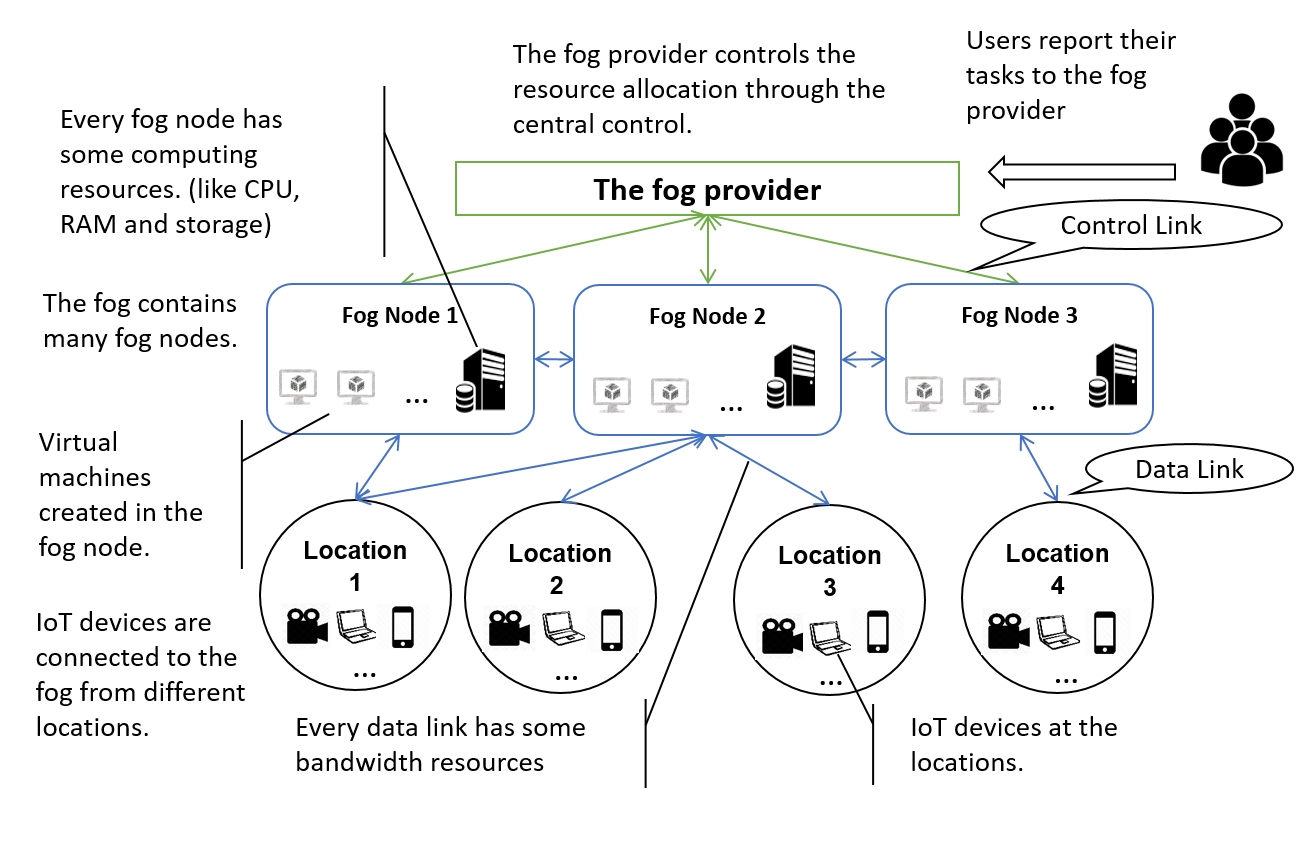
\includegraphics[width=1.0\textwidth]{./Figures/system_structure.png}
    \caption{\label{fig:system_structure} General view of a fog computing system.}
\end{figure}

Another essential part of our model are fog users. They report their tasks (e.g., a video surveillance task or a picture processing task) to the fog provider through their IoT devices over time (Figure \ref{fig: procedure}), which includes the resource requirements, the time constraints and the valuation functions of the tasks. For example, a picture processing application can have computing tasks like adding filters or compressing photos. To finish a task of adding filters to 100 photos, bandwidth resources are needed to send the images to and from the FN, and computational resources are needed to process the image. The time constraints of this task could be like this: the task can start right now, and the result should be sent to the user in 30 seconds because users usually do not want to wait for too long to add a filter to their photos. If the task is completely finished before the deadline, the user can get all the value of this task. However, if filters have only been added to 50 photos at the deadline, it is reasonable that the user can still get part of the value of this task. 
%Since fog users are generally not technical experts, and they often do not know the precise amount of resources needed for their tasks. Therefore, the applications will automatically generate the computational and bandwidth resources demands (i.e., the computational resources for the VM and the bandwidth resources between the VM and locations) for them.
% Here, we assume that one task only needs one VM. Finally, the application will submit the complete bid to the fog provider.

When receiving the reports from the applications, the fog provider decides whether to accept them, how to allocate resources to satisfy the demands of the accepted tasks and how much is the corresponding payment through an online mechanism (Figure \ref{fig: procedure}). Finally, the social welfare of the allocation is the sum of value fog users get by processing tasks minus the sum of the fog provider's operational costs, while the revenue is the sum of the fog provider's income minus its operational costs. We focus on social welfare because we assume that the fog provider is a non-profit organisation, and improving overall social welfare is its primary objective. Therefore, we leave the objective of maximising the fog provider’s revenue to future work.

\begin{figure}
    \centering
    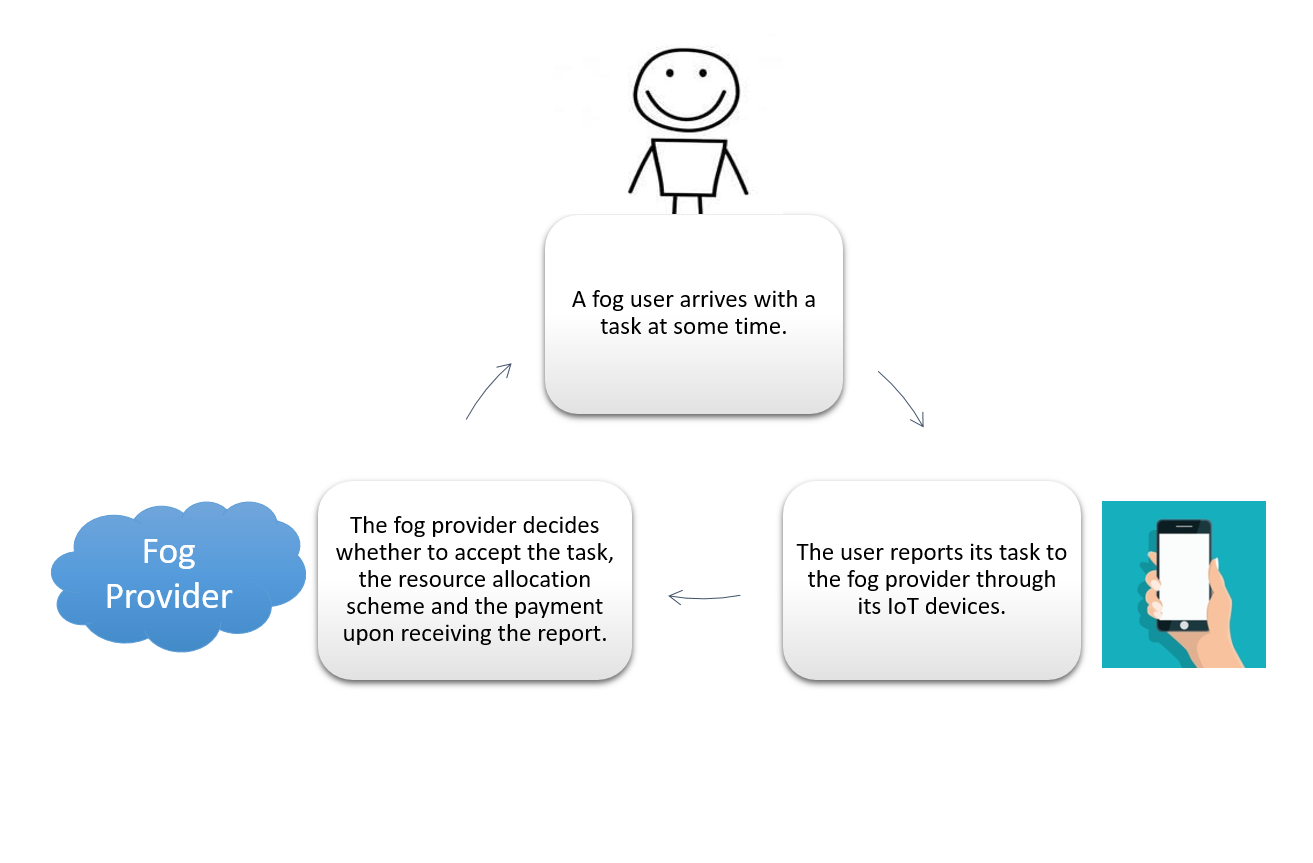
\includegraphics[width=1\textwidth]{./Figures/Allocation_procedure.png}
    \caption{\label{fig: procedure} The procedure of RAFC.}
\end{figure}

\subsection{Formal Model} \label{formal model}

We now present the model described in Section \ref{overview of the model} in detail and formally. Consider a fog provider with a set $W$ of geo-distributed FNs and a set $L$ of locations, which are interconnected through a set $\mathbb{E}$ of data links, as shown in Figure~\ref{fig:system_structure}. 

Furthermore, there is a set $ E_l $ of IoT devices in each location $ l $, and $ e \in E_l $ is an IoT device (e.g., a smart TV, surveillance camera, smart speaker or AV). Every FN $w \in W$ has a set $R$ of limited computational resources (e.g., CPU, RAM and storage). Moreover, there are $A_{w,r}$ units of type $r \in R$ resources in FN $w$, and the unit operational cost of resource $r$ in FN $w$ is $o_{w,r}$. In addition, the bandwidth capacity and the unit operational cost of link $(j, k) \in \mathbb{E}$ are $b_{j,k}$ and $o_{j,k}$ respectively. 
%The operational costs of computational resources mainly comprise electricity costs and the depreciation charge of the resources, and the operational costs of bandwidth resources are the costs charged by network operators. 
For simplicity, we assume that the bandwidth capacity and unit bandwidth costs are symmetrical for all links (i.e., $b_{j,k} = b_{k,j},\ o_{j,k} = o_{k,j}, \  \forall (j,k)\in \mathbb{E} $). FNs and data links together offer their resources to satisfy the needs of fog users. 
In particular, we assume that VMs can be created in an FN to run computing tasks as long as there are enough computational resources in that FN, and the total resource requirements of several virtual machines are just the sum of their individual resource requirement for simplicity, although, in reality, they may need fewer resources because they can share resource with each other. 
Furthermore, the fog provider uses a centralised online resource allocation mechanism to make resource allocation decisions.
%Furthermore, the fog provider controls the resource allocation of the fog through a central control system, and we focus on centralised resource allocation mechanisms.

Fog users with tasks arrive over time, and $I$ denotes the set of all tasks. Note that we adopt a continuous time system, but the tasks can only start execution at discrete time steps, denoted by the set $ T = \{1,2,\ldots,|T|\} $. Each task $i \in I$ is owned by a user,  which is also denoted as $i$ for simplicity because we assume that each user has one task. In addition, the arrival time of task $i$ is $T_i^a \in [0, |T|] $, which is the time when user $i$ becomes aware of its task $ i $, and the time window that the task can be processed is from its start time $ T_i^s $ to its deadline $ T_i^d $. Here, we assume that no tasks arrive at the exact same time. User $i$ reports its task's type $ \hat{\theta}_i $ (as defined in the following) at time $\hat{T}_i^a$ to run a certain application (e.g., a video surveillance application or a picture processing application). We assume that user $i$ wants to know the number of time steps $ \tilde{t}_i $ it will get and the payment $ p_i$ for its task also by time $\hat{T}_i^a$ because users want to run the tasks locally or elsewhere if their tasks get rejected. The operational cost of task $ i $ is denoted as $ o_i $, which is the sum of costs of all resources allocated to task $ i $, including the cost of bandwidth. Furthermore, we also assume that every task only requires one VM to run but may require connections to several endpoints $ e \in E$ (in the same location or in different locations) because this is common in an IoT system~\citep{du2018computation}. Users are also assumed to be stationary, which means that the endpoints of users do not change locations over time. Furthermore, we also assume VMs can migrate between FNs and the migration costs are negligible, and all tasks are preemptible, which means that they can always be paused and resumed. Finally, we focus on one type of task called time-oriented tasks (e.g., video surveillance and video processing tasks), which are common in fog computing. Such a task $i$ needs a certain configuration of resources for a time length $t_i$ to get its full value, but can still get part of the value if the processing time is less than $t_i$. Formally, the type of task $i$ is a tuple $\theta_i = (T_i^a, T_i^s, T_i^d, v_i, \{ a_{i,r} \}_{r \in R}, \{ \Gamma_l^i \}_{l \in L} )$, where $a_{i,r}$ denotes the amount of resource $r \in R$ required, and $ \Gamma_l^i$ denotes the bandwidth demand between its VM and location $l \in L$. For simplicity, bandwidth demands are symmetrical. That is, $\Gamma_l^i$ denotes both the bandwidth demands to and from location $l \in L$. In this paper, the valuation function is given by $ v_i = \{v_{i,0}, v_{i,1},\ldots,v_{i,t_i}\} $, where $ v_{i,t} $ is the value when task $ i $ gets a usage time of $ t $ time steps within its time window ($ [T_i^s, T_i^d] $) and $t_i$ denotes the usage time needed to get the full value of the task. We make the reasonable assumption that the valuation function monotonically increases with usage time (i.e., $ v_{i,t''} \geq v_{i,t'} \quad \forall t'' \geq t' $). For example, suppose a user wants to run a real-time video analytics application with facial recognition to surveil their shops for 24 hours. It is intuitive that they will not get additional value for a surveillance time of more than 24 hours, and it is still of value to them if the surveillance lasts less than 24 hours, say, 18 hours. We choose this type of valuation function because it corresponds to many applications in the fog, which achieve better results as processing time increases. Moreover, the reported type of task $i$ is a tuple $\hat{\theta}_i = (\hat{T}_i^a, \hat{T}_i^s, \hat{T}_i^d, \hat{v}_i, \{ \hat{a}_{i,r} \}_{r \in R}, \{ \hat{\Gamma}_l^i \}_{l \in L})$, and $ \hat{\theta}^{\langle t \rangle} $ denotes the set of all reported types until and including time step $ t $. 

%Furthermore, we adopt a discrete time system, and the set of discrete time periods is denoted as $T$. In addition, we assume that the fog users' tasks appear according to a Poisson process, and the arrival time of task $n$ is $T_n^a$. A bid for task $n\in N$ is submitted at time $\hat{T}_n^a$ by a user to run a certain application, and we assume that no two tasks are submitted simultaneously (i.e., $\hat{T}_{n_1}^a \neq \hat{T}_{n_2}^a, \quad \forall {n_1},n_2 \in N$).
%We also assume that every task only requires one VM to run but may require several IoT devices, and all IoT devices $ e \in E_l$ at location $l \in L$ share the bandwidth between $l$ and the fog. $e$ denotes an IoT device and $E_l$ is the set of all IoT devices at location $l$. Furthermore, users are assumed to be stationary, which means that the IoT devices of users do not change locations over time. Finally, we only consider one type of tasks called time-oriented tasks (e.g., fingerprint identification, facial recognition and video processing), which means that the task $n$ needs an invariable capacity of resources for a continuous time length $t_n$, within a time duration $[T_n^s, T_n^f]$. In short, the type of task $n$: $\theta_n$ is a tuple $(T_n^a, T_n^s, T_n^f,t_n ,v_n)$, in which the valuation function $v_n$ is assumed to be a non-decreasing linear function of the actual running time within the time duration:
%\[ v_n(t_n') =
%\begin{cases}
%g_n \times t_n' & \text{if} \; t_n' \leq t_n  \\
%g_n \times t_n  &    \text{if} \; t_n' > t_n
%\end{cases}
%\]
%where $g_n$ is the coefficient, $t_n' = min( {T_n^f}' - {T_n^s}', T_n^f - {T_n^s}' )$ is the scheduled usage time for task $n$, and ${T_n^s}', {T_n^f}'$ are the scheduled start time and deadline for task $n$ respectively. This type of valuation function corresponds to general analytical applications, which often have better results as process time increases. For example, suppose we use an artificial neural network (ANN) to learn somebody's face in a facial recognition application, the more time the ANN is trained the higher its rate of accuracy will be. Figure \ref{fig:function} shows a rough graph of such a valuation function. 
%% A user's value for a task is reflected by the valuation function and the different operational costs among all possible schemes of resource allocations. For example, if the user uses a video surveillance application, the bandwidths between the VM and the IoT devices are high. This user prefers to allocate the VM in an FN near the locations of IoT devices. 
%However, the users can be strategic. The bid for task $n$: $\hat{\theta}_n$ = ($ \hat{T}_n^a,\hat{T}_n^s,\hat{T}_n^f,\hat{t}_n, \hat{v}_n $) may be different from the task's truth type: $\theta_n$ = ($T_n^a, T_n^s, T_n^f,t_n ,v_n$). Moreover, we assume limited misreports based on the nature of our problem (i.e., $\hat{T}_n^a \geq T_n^a, \hat{T}_n^s \geq T_n^s, \hat{T}_n^f \leq T_n^f, \hat{t}_n \leq t_n$). This is because a user cannot bid for a task before it has this task. It also cannot bid a looser time constraint for the task, because this behaviour may be detected by the fog provider if the task is allocated outside the truth time constraint. 
%% Second, a user will not report an earlier start time, a later deadline or a longer usage time for its task, i.e., it must hold that $\hat{T}_n^s \geq T_n^s, \hat{T}_n^f \leq T_n^f, \hat{t}_n \leq t_n$. 
%% (Need thinking, can they bid an earlier start time?)

Now, a key assumption in our work is that users are strategic, so $\hat{\theta}_i$ may not be the same as $ \theta_i $. Moreover, we assume limited misreports (see Section \ref{direct-revelation online mechanisms}) based on the nature of our problem (i.e., $\hat{T}_i^a \geq T_i^a, \hat{T}_i^s \geq T_i^s, \hat{T}_i^d \leq T_i^d, \hat{a}_{i,r} \geq a_{i,r} \, r\in R, \hat{\Gamma}_l^i \geq \Gamma_l^i  \, l \in L $). This is reasonable because a user cannot report a task before it becomes aware of it (i.e., $ \hat{T}_i^a < T_i^a $), and cannot report a looser time window (i.e., $\hat{T}_i^s < T_i^s$ or $\hat{T}_i^d > T_i^d$) because the fog provider can check whether task $ i $ is ready to be processed at $ \hat{T}_i^s $ and withhold the results for $ i $ until $ \hat{T}_i^d $. So reporting $\hat{T}_i^s < T_i^s$ will be detected and penalised by cancelling the task and reporting $\hat{T}_i^d > T_i^d$ will result in no value. 
%For tasks that cannot withhold results, FlexOG mechanism is not DSIC anymore, but OG and SWMOA2 mechanisms (they are benchmarks introduced in the next section) are still DSIC. The proof is omitted for space reasons. 
Finally, user $ i $ will not misreport a lower resource requirement because its task cannot be processed in that case. However, for some tasks, the results cannot be withheld until the deadline of the tasks such as video surveillance tasks and autopilot tasks. This situation is discussed in Section \ref{late deadline}.

Next, when receiving the bid $ \hat{\theta}_i $ for task $i$, the fog provider will decide the resource allocation scheme $ \lambda_i$, which is a tuple formally defined in the later part of this paragraph, right away to this task including how much usage time $ \tilde{t}_i $ will be allocated, and the payment $ p_i$  because of the assumption we made earlier that all users want to know the allocation results at their arrival times. To provide an upper bound on the social welfare, we find the optimal social welfare in an offline setting by solving a constraint optimisation problem, and the decision variables are: (1) $\{ z_{w,t} ^i \in \{ 0, 1 \} \}_{i \in I, w \in W, t \in T}$, indicating that the VM of task $i$ is placed in FN $w$ $(z_{w,t} ^{i} = 1)$, or not $(z_{w,t}^i =0)$ at time step $t$. (2) $\{ f_{l,w,j,k,t}^i \in \mathbb{R}^+ \}_{ i \in I, l \in L, w \in W, (j, k) \in \mathbb{E}, t \in  T }$, indicating allocation of the bandwidth on link $ (j,k) $ for traffic from location $ l $ to FN $ w $ for task $i$ at time step $t$.  So, for task $i$, its usage time $\tilde{t}_i = \underset{w\in W, t\in T} {\sum}z_{w,t}^i$ and resource allocation scheme $ \lambda_i = ( \{ z_{w,t} ^i  \}_{i \in I, w \in W, t \in T} , \{ f_{l,w,j,k,t}^i \}_{ i \in I, l \in L, w \in W, (j, k ) \in \mathbb{E}, t \in  T } )$. The objective function (\ref{eq: constraint_optimisation_problem}) of this optimisation problem maximises the social welfare, which is subject to resource and time constraints:

\small
 \begin{maxi!}
     {\lambda_i}{\sum_{i \in I} v_i (\sum_{ w \in W, t\in T} z_{w,t}^i ) -(\sum_{i \in I, r \in R,w \in W, t\in T} a_{i,r} z_{w,t}^i o_{w,r}
          + \sum_{i \in I, l \in L,w \in W,(j,k) \in \mathbb{E}, t\in T} 2  o_{j,k}  f_{l,w, j,k,t}^i )}{}{\label{eq: constraint_optimisation_problem}} 
    \addConstraint{\sum_{w \in W} z_{w,t}^i}{\leq  1\quad \forall i \in I, t \in T}{\label{eq:2}}
    \addConstraint{\sum_{i \in I} z_{w,t}^i a_{i,r}}{\leq A_{w,r} \quad \forall w \in W, r \in R, t \in  T}{\label{eq:3}}
    \addConstraint{z_{w,t}^i}{= 0 \quad \forall i \in I, w \in W, t < T_i^s \, or \, t > T_i^d}{\label{eq:4}}
    \addConstraint{\sum_{j:(j,w) \in \mathbb{E}} f_{l,w,j,p,t}^i}{= \Gamma_l^i z_{w,t}^i \quad \forall w \in W, i \in I, l \in L, t \in T}{\label{eq:5}}
    \addConstraint{\sum_{k:(l,k) \in \mathbb{E}} f_{l,w,l,k,t}^i}{= \Gamma_l^i z_{w,t}^i \quad \forall w \in W, i \in I, l \in L, t \in T}{\label{eq:6}}
    \addConstraint{\sum_{j:(j,k) \in \mathbb{E}} f_{l,w,j,k,t}^i}{= \sum_{j:(k,j) \in \mathbb{E}} f_{l,w,k,j,t}^i \quad \forall w \in W,k \in W, i \in I, l \in L, t \in T}{\label{eq:7}}
    \addConstraint{\sum_{i \in I} f_{l,w,j,k,t}^i}{\leq b_{j,k} \quad \forall (j,k)\in \mathbb{E}, t \in T}{\label{eq:8}}
    \addConstraint{f_{l,w,j,k,t}^i}{\geq 0 \quad \forall i \in I, l \in L, w \in W, (j,k) \in \mathbb{E}, t \in T}{\label{eq:9}}
\end{maxi!}

\normalsize
To explain the above constraints in detail, constraint (\ref{eq:2}) represents that every task only needs one VM. Constraint (\ref{eq:3}) guarantees that at each time step the allocated resources at any FN do not exceed its resource capacities. Constraint (\ref{eq:4}) means that the VM is created within the start time and deadline of the task. Constraint (\ref{eq:5}) requires that the total inbound traffic to FN $w$ for the traffic from task $i$'s location $l$ equals its corresponding bandwidth demand at each time step if the VM for task $i$ is placed in FN $w$. 
%$ \Gamma_l^i $ denotes the bandwidth demands both from location $ l $ and to location $ l $ because the bandwidth demands are assumed to be symmetrical (i.e., the bandwidth demands for task $i$ from its VM to location $l$ and from location $l$ to its VM are both equal to $\Gamma_l^i$). 
Since the bandwidth demands and the bandwidth costs are both symmetrical. It is sufficient to just consider the traffic from $ L $ to $ W $. Constraint (\ref{eq:6}) indicates that the outbound traffic from task $i$'s location $l$ is equal to its corresponding bandwidth demand at each time step. Constraint (\ref{eq:7}) represents that the inbound and outbound traffic of intermediate nodes for task $ i $ should be equal. Constraint (\ref{eq:8}) guarantees that the aggregated traffic on each link does not exceed its bandwidth capacity at each time step. Finally, constraint (\ref{eq:9}) ensures that the allocated bandwidth in each data link is not negative, which is impossible in practice. 

This is a mixed integer linear programming problem (MILP) because the objective function and the constraints are linear and one of the decision variables $ z_{w,t} ^i $ is discrete. Unfortunately, this problem is NP-hard, which can be proved by reducing a 0-1 knapsack problem to it (see detailed proof below). In practice, the optimisation problem (\ref{eq: constraint_optimisation_problem}) can be solved using linear programming solvers. In particular, we use the IBM ILOG CPLEX Optimization Studio to solve it. However, solving this problem can be time-consuming because the problem is hard per se.

\begin{theorem} \label{th: NP-hardness}
    The optimisation problem (\ref{eq: constraint_optimisation_problem}) is NP-hard.
\end{theorem}

\begin{proof}
    Suppose we have a 0-1 knapsack problem with a maximum weight capacity $ A_w $ and $ |I| $ items with weights $ \{ a_i \}_{i \in I} $ and values $ \{ v_i \}_{i \in I} $. We can design a fog computing resource allocation problem as follows. There is one FN with CPU resource $ A_w $ and no other resources. All $ |I| $ tasks arrives at $ t = 0 $ and task $ i $ requires only $  a_i $ CPU resource with start time $ T_i^s = 0 $, deadline $ T_i^d = 1 $, and value $ v_i, i \in I $ for $ t_i=1 $. Then, we can solve the above 0-1 knapsack problem by just solving the above fog computing resource allocation problem. Ergo, the offline optimal problem is at least as hard as the 0-1 knapsack problem. Since the optimisation problem of a 0-1 knapsack problem is NP-hard, the optimisation problem (\ref{eq: constraint_optimisation_problem}) is NP-hard too.
\end{proof}

Finally, since mechanisms need to make both resource allocation decisions and payment decisions for fog users. We use $p_i(\lambda_i, \hat{\theta}^{\langle \hat{T}_i^a \rangle}) \in \mathbb{R}^+ $ to denote the payment of task $i$, which is a function of the allocation: $ \lambda_i  $ and all information received by $ \hat{T}_i^a $: $ \hat{\theta}^{\langle \hat{T}_i^a \rangle} $. Thus the usitlity of user $ i $ is $ u_i = v_i(\tilde{t}_i) - p_i(\lambda_i, \hat{\theta}^{\langle \hat{T}_i^a \rangle})$, and this is what user $ i $ tries to maximise.

\section{Price-based Mechanisms} \label{price-based mechanisms}

First, we introduce a class of online resource allocation mechanisms called price-based mechanisms that guarantee DSIC and IR for our resource allocation problem because our proposed mechanism belongs to it. Note that this class of mechanisms is an adaptation from the price-based mechanisms characterised by~\citet{hayakawa2018price}. In the following, we characterise the properties that this class of mechanisms should have, in order to guarantee DSIC and IR.

\begin{definition}\label{df: monotonicity}
    A monotonic payment function is (weakly) monotonically increasing over $\hat{T}_i^a$, $\hat{T}_i^s$, $ \hat{t}_i $, $ \hat{a}_{i,r}, r \in R $ and $  \hat{\Gamma}_l^i, l \in L $, and (weakly) monotonically decreasing over $\hat{T}_i^d$.
\end{definition}

Then, we define the class of price-based mechanisms for our RAFC problem as follows:

\begin{definition}\label{df: price-based}
    An online mechanism belongs to the price-based mechanisms class if it has the following properties:
    \begin{enumerate}
        \item The mechanism computes the payment $ p_i$ for any possible allocation $ \lambda_i $ to task $i$ by using a payment function $p_i(\lambda_i, \hat{\theta}^{\langle \hat{T}_i^a \rangle})$ that is independent of $\hat{v}_i$ and monotonic.
        %        
        \item The resource allocation scheme $\lambda_i$ for task $ i $ maximises $ \hat{v}_i(\lambda_i) - p_i(\lambda_i, \hat{\theta}^{\langle \hat{T}_i^a \rangle})$ (over all $\lambda_i$ that can be made to task $i$ for any $\hat{v}_i$).
        \item The payment for tasks with no resource allocated is zero.
    \end{enumerate}
\end{definition}

Then, the following theorem guarantees that any mechanism in the class of price-based mechanisms is DSIC and IR.

\begin{theorem}\label{th: DSICandIR}
    Any online mechanism that satisfies Definition \ref{df: price-based} is DSIC and IR.
\end{theorem}

\begin{proof}
    The proof is shown below.
\end{proof}

To prove a mechanism that satisfies the Definition \ref{df: price-based} is DSIC, we first use the sufficient and necessary characterisation of incentive compatible mechanisms for a setting where users can only misreport their valuation function (i.e., where the misreports of $\hat{T}_i^a$, $\hat{T}_i^s$, $\hat{T}_i^d$, $ \hat{t}_i $, $ \{ \hat{a}_{i,r} \}_{r \in R} $ and $ \{ \hat{\Gamma}_l^i \}_{l \in L} $ are not considered) proposed by \citet{bartal2003incentive} .

\begin{lemma}\label{lm:Bartal}
    In our setting, assuming the parameters $\hat{T}_i^a$, $\hat{T}_i^s$, $\hat{T}_i^d$, $ \hat{t}_i $, $ \{ \hat{a}_{i,r} \}_{r \in R} $, $ \{ \hat{\Gamma}_l^i \}_{l \in L} $ in user $ i $'s bid $ \hat{\theta}_i $ are truthful, a direct revelation mechanism is DSIC if and only if
    
    \begin{enumerate}
        \item The payment function $p_i(\tilde{t}_i, \hat{\theta}^{\langle \hat{T}_i^a \rangle})
        $ is computed for every possible allocation $ \tilde{t}_i $ for task $i$ and does not depend on $\hat{v}_i$.
        \item The allocation function allocates $\tilde{t}_i$ for task $i$ such that the value of $\hat{v}_i( \tilde{t}_i)-p_i(\tilde{t}_i, \hat{\theta}^{\langle \hat{T}_i^a \rangle}) $ is maximised (over all $\tilde{t}_i$ that can be allocated to $i$ for any choice of $\hat{v}_i$).
    \end{enumerate}
\end{lemma}

Lemma \ref{lm:Bartal} is an simple extension of Theorem 1 in \citep{bartal2003incentive}. 

Then, we use this Lemma to prove the following theorem that is in settings where users can misreport $ \hat{T}_i^a,\hat{T}_i^s,\hat{T}_i^d $, $ \hat{t}_i $, $ \{ \hat{a}_{i,r} \}_{r \in R} $, $ \{ \hat{\Gamma}_l^i \}_{l \in L} $ besides $\hat{v}_i$ (assuming limited misreports).

\begin{theorem} \label{th: DSIC}
    In our setting, a direct revelation mechanism is DSIC if and only if
    \begin{enumerate}
        \item The payment function $p_i(\tilde{t}_i, \hat{\theta}^{\langle \hat{T}_i^a \rangle}) $ for every possible allocation $ \lambda $ to task $i$ is monotonic and does not depend on $\hat{v}_i$.
        \item The allocation function allocates $ \tilde{t}_i  $ for task $i$ such that the value of $\hat{v}_i( \tilde{t}_i)-p_i(\tilde{t}_i, \hat{\theta}^{\langle \hat{T}_i^a \rangle}) $ is maximised (over all $ \tilde{t}_i$ that can be allocated to $i$ for any choice of $\hat{v}_i$).
    \end{enumerate}
\end{theorem}

\begin{proof}
    At first, we show that the conditions in Theorem \ref{th: DSIC} are sufficient. According to Lemma \ref{lm:Bartal}, a user $ i $ cannot increase its utility by manipulating $\hat{v}_i$. Therefore, we can assume that it truthfully reports its valuation coefficient $\hat{v}_i$, and the only way to increase its utility is by decreasing the payment function. Since the payment function is monotonic, only misreporting $\hat{T}_i^a < T_i^a, \hat{T}_i^s < T_i^s, \hat{T}_i^d > T_i^d$, $ \hat{t}_i < t_i $, $ \hat{a}_{i,r}  <  a_{i,r}, r \in R  $ or $   \hat{\Gamma}_l^i  <  \Gamma_l^i , l \in L  $ can reduce it. First of all, misreporting $\hat{T}_i^a < T_i^a, \hat{T}_i^s < T_i^s, \hat{T}_i^d > T_i^d$ is impossible because the limited misreports assumption we made earlier. Then, misreporting $ \hat{t}_i < t_i $ only reduces $ u_i $ because of condition two. Finally, misreporting $ \hat{a}_{i,r}  <  a_{i,r} \ r \in R  $ or $   \hat{\Gamma}_l^i  <  \Gamma_l^i \  l \in L  $ will lead to the failure of the task, which reduces $ u_i $ to negative. Hence, user $ i $ has no incentive to submit a non-truthful bid (i.e.,  ($\hat{T}_i^a,\hat{T}_i^s,\hat{T}_i^d, \hat{v}_i, \{ \hat{a}_{i,r} \}_{r \in R} $, $ \{ \hat{\Gamma}_l^i \}_{l \in L} $) $ \neq $ ( $T_i^a, T_i^s, T_i^d, v_i $, $ \{ a_{i,r} \}_{r \in R} $, $ \{ \Gamma_l^i \}_{l \in L} $)).
    
    %    \todo{are these conditions really necessary?}
    Then, we show that the conditions in theorem \ref{th: DSIC} are also necessary. We first assume to the contrary that the first condition does not hold, i.e., the payment function is not independent of $\hat{v}_i$ or the payment function is not \textit{monotonic}. In the former case, the mechanism is not DSIC according to Lemma \ref{lm:Bartal}. In the latter case, that is, there is some ${T_i^a}' < {T_i^a}''$ such that the resource allocation is the same $( \lambda' = \lambda'' )$ but the payment satisfies $p_i(\lambda', {T_i^a}') > p_i(\lambda'', {T_i^a}'')$, while $\hat{T}_i^s$ and $\hat{T}_i^d$ remain unchanged. On this occasion, a user whose true arrival time is ${T_i^a}'$ and who gets allocation $ \lambda' $ when reporting truthfully is incentivised to misreport ${T_i^a}'$ as ${T_i^a}''$ because it can get the same allocation with less payment. Since this is contrary to the definition of DSIC, the first condition must be necessary.
    
    Then, we assume that the first condition holds, but to the contrary that the second condition does not. For instance, for some user $ i $ with $ v_i = v_i'$ , there exists $v_i''$, the mechanism allocates $\lambda_i'$ and $\lambda_i''$ respectively such that $v_i' (\tilde{t}_i') - p_i(\lambda_i', \hat{\theta}^{\langle \hat{T}_i^a \rangle}) < v_i'' (\tilde{t}_i'') - p_i(\lambda_i'', \hat{\theta}^{\langle \hat{T}_i^a \rangle}) $. On this occasion, this user is incentivised to misreport  $v_i'$ as $ v_i'' $. Hence, the second condition is also necessary.
    
    Finally, a mechanism that satisfies the Definition \ref{df: price-based} is also IR for the following reasons. Since user $ i $ will always bid truthfully (i.e., $ \hat{v}(t) = v(t) $), the final allocation actually maximises the utility of user $i$: $ u_i = v_i(\tilde{t}_i)-p_i$. In addition, the maximum of $ u_i $ should be greater or equal to zero as $i$ can always get a utility of zero with no resource allocated according to condition 3 in Definition \ref{df: price-based}. From the above discussion, it is clear that $i$ will never get a negative utility under such mechanisms.
    
    From the above, Theorem \ref{th: DSIC} is proven, and so is Theorem \ref{th: DSICandIR}.
\end{proof}

\section{Resource Allocation Benchmark Mechanisms} \label{benchmarks}

% In this section, the offline optimal mechanism and three truthful online mechanisms for RAFC are presented. The first three mechanisms are used as benchmark mechanisms to evaluate the last mechanism.

Against this background, we present the benchmark mechanisms and the mechanism we proposed for RAFC. We choose four benchmark mechanisms: the offline optimal mechanism represents the upper bound of social welfare efficiency; the online optimal mechanism is a representative online heuristic mechanism; the online greedy mechanism is a representative truthful online heuristic mechanism; and Social Welfare Maximisation Online Auction 2 (SWMOA2) is a variant of a state-of-the-art truthful online mechanism called Social Welfare Maximisation Online Auction (SWMOA)~\citep{shi2017online}. 



%\begin{equation} \label{eq:SWM}
%\underset{{T_n^t}', z_{w,t} ^{n}, f_{l,w,w_i,w_j,t}^n \quad l \in L, w \in W, (w_i,w_j) \in \mathbb{E}, t \in  T}{\text{maximise}}    \sum_{n\in N,w \in W, t\in T} (v_n(z_{w,t} ^n)-o_n)
%\end{equation}
%\begin{subequations}
%\begin{align}
%\text{s.t.} \quad  \sum_{w \in W} z_{w,t}^n &\leq  1 \quad \forall n\in  N, t \in  T\\
%\sum_{n\in  N} z_{w,t}^n a_{n,r} &\leq A_{w,r} \quad \forall w \in W, r \in R, t \in T \\
%z_{w,t}^n &= 0 \quad \forall n\in N, w \in W, t < T_n^s \, or \, t > T_n^f\\
%\sum_{t = 2}^{|T|} ( \sum_{w \in W} z_{w,t}^n - \sum_{w \in W} z_{w,t-1}^n )^2 &\leq 2 \quad \forall n \in N \\
%\sum_{w\in W} \sum_{t \in T} z_{w,t}^n &= \max_{w\in W} \sum_{t \in  T} z_{w,t}^n \quad \forall n \in N\\
%\sum_{w:(w,p) \in \mathbb{E}} f_{l,w,w,p,t}^n &= \Gamma_l^n z_{w,t}^n \quad \forall w \in W, n \in  N, l \in L, t \in  T \\
%\sum_{w:(l,w) \in \mathbb{E}} f_{l,w,l,w,t}^n &= \Gamma_l^n z_{w,t}^n \quad \forall w \in W, n \in  N, l \in L, t \in  T \\
%\sum_{w_i:(w_i,w_j) \in \mathbb{E}, w_j \notin \{l, p\}} f_{l,w,w_i,w_j,t}^n &= \sum_{w_i:(w_i,w_j) \in \mathbb{E}, w_j \notin \{l, p\}} f_{l,w,w_j,w_i,t}^n \quad \forall w \in W, n \in  N, l \in L, t \in  T \\
%\sum_{n\in  N, l\in L,w \in W} f_{l,w,w_i,w_j,t}^n &\leq b_{w_i,w_j} \quad \forall (w_i,w_j)\in \mathbb{E}, t \in  T\\
%f_{l,w,w_i,w_j,t}^n &\geq 0 \quad \forall n \in  N, l \in L, w \in W, (w_i,w_j) \in \mathbb{E}, t \in  T\\
%o_n &= \sum_{r \in R,w \in W, t\in T}(a_{n,r} z_{w,t}^n o_{w,r}) \nonumber \\ & + \sum_{l \in L,w \in W,(w_i,w_j) \in \mathbb{E}, t\in T}(2o_{w_i,w_j} \times f_{l,w, w_i,w_j,t}^n) \quad \forall n \in N
%\end{align}
%\end{subequations}
%
%The objective in $(1)$ is to maximise the social welfare. Constraint $(3.2a)$ represents that every task only needs one VM. Constraint $(3.2b)$ guarantees that at each time step the allocated resources at any FN do not exceed its resource capacities. Constraint $(3.2c)$ means that the VM is created within the start and deadline of the task. Constraint $(3.2d)$ means that any VM runs in a continuous time stretch. Constraint $(3.2e)$ shows that no VM migration is allowed. However, these two constraints make the programme non-linear. We tried to find linear constraints to replace them, but we have not found one. We will try to solve this problem in our future work. Constraint $(3.2f)$ requires that the total inbound traffic to FN $w$ for the traffic from task $n$'s location $l$ equals its corresponding bandwidth demand at each time step if the VM for task $n$ is placed in FN $w$. Because the bandwidth demand is assumed to be symmetrical (i.e., the bandwidth demands for task $n$ from its VM to location $l$ and from location $l$ to its VM both equal to $\Gamma_l^n$) and the bandwidth costs are also symmetrical (i.e., $o_{w_i,w_j} = o_{w_j,w_i}$), it is sufficient to just consider the traffic from locations to FNs. Constraint $(3.2g)$ indicates that the outbound traffic from task $n$'s location $l$ is equal to its corresponding bandwidth demand at each time step. Constraint $(3.2h)$ represents that the inbound and outbound traffic of intermediate nodes should be equal. Constraint $(3.2i)$ guarantees that the aggregated traffic on each link does not exceed its bandwidth capacity at each time step. Constraint $(3.2j)$ guarantees that the amount of allocated bandwidth is not negative, which is impossible in practice. The last equation computes the total operational cost of task $n$. It consists of two parts: the costs of computational resources at FNs and the cost of bandwidths on links. This is not a linear problem because of constraints $(3.2d)$ and $(3.2e)$.

% https://www.cnblogs.com/wanghetao/archive/2012/03/31/2427625.html
% The above offline optimisation problem is a combination of the offline VM placement problem and the bandwidth allocation problem. An offline problem is solved after getting all the input data, while an online problem is solved piece-by-piece during the receiving of the input data \citep{karp1992line}. Because it does not know the whole input, the result of an online problem often turns out not to be optimal in hindsight. The offline VM placement problem, which is a variant of the multi-dimensional multiple knapsack problem, is to maximise the social welfare by only considering the allocation of VMs and ignoring the allocation of bandwidths. The aim of the multi-dimensional multiple knapsack problem is to maximise the value of items put in multiple knapsacks, given a set of items. The weights of items and the capacities of knapsacks are more than one dimension. Similarly, in the offline VM placement problem, the objective is to maximise the total social welfare of tasks without overloading any FNs at any time. The VMs are similar to items, and the FNs are similar to knapsacks here. Moreover, in our problem, the resource demands of VMs and the resource capacity of FNs are multi-dimensional. The difference is that the objective of the offline VM placement problem is to maximise the total social welfare in a period of time instead of a single allocation.

% The problem of bandwidth allocation, which is to minimise the bandwidth costs given the VM placement of tasks, is a minimum cost multi-commodity flow problem. The objective of the minimum cost multi-commodity flow problem is to minimise the link cost subject to multiple flow demands between different source and sink nodes. Similarly, in the bandwidth allocation problem locations and FNs of the tasks can be regarded as source and sink nodes.
% Since bandwidth demands, which are bidirectional, on each data link are assumed to be symmetrical, they can be treated as flow demands. The objective is also minimising the link cost. Since fractional flows are allowed in our model, the problem can be solved in polynomial time through linear programming, or through fully polynomial time approximation schemes.
\subsection{Offline Optimal Mechanism}
Under this mechanism, we assume that we know all the information about future tasks and allocate resources to optimise the social welfare with no need to incentivise fog users to report their tasks truthfully. This theoretical and idealised case can be achieved by solving the constraint optimisation problem \ref{eq: constraint_optimisation_problem} in Section~\ref{formal model}.

\subsection{Online Optimal Mechanism}
This mechanism is similar to the offline optimal mechanism except that the optimisation problem is solved at each time step with knowledge only of the tasks that have arrived so far (and not of future tasks). Note that this mechanism is not truthful, but we use this to determine the social welfare that could be achieved in an online setting if all users report truthfully. In Section \ref{utility evaluation}, we also evaluate this mechanism's performance in social welfare in settings where part of users misreport. The details of this mechanism is given in Algorithm \ref{alg: ono} below.

\begin{algorithm}
    %    \scriptsize
    %    \setstretch{0.7}
    \SetAlgoLined
    \DontPrintSemicolon
    \caption{The online optimal mechanism} \label{alg: ono}
    $\theta_{arrived} \gets \emptyset$ \Comment*[r]{The set of arrived tasks} 
    $\theta_{unf} \gets \emptyset$ \Comment*[r]{The set of unfinished tasks} 
    %    $ o \gets 0 $ \Comment*[r]{The total operational costs} 
    %    $\tilde{T} \gets \emptyset$ \Comment*[r]{The set of committed processing times} 
    
    
    \For{$t$ in $T$}{
        \While{ new tasks arrive within $ t $}{
            When a new task $ i $ arrives \Comment*[r]{Tasks arrive over time} 
            $\theta_{arrived} \gets \theta_{arrived} \cup i$ \Comment*[r]{Update the set of arrived tasks} 
            $\theta_{flex} \gets \theta_{flex} \cup i$ \Comment*[r]{Update the set of unfinished tasks} 
        }
        Solve the maximum utility allocation for tasks in $ \theta_{unf} $ 
        (i.e., $ \underset{\lambda_j}{\argmax} \underset{j\in \theta_{unf}}{\sum}(\hat{v}_j(\lambda_j) - o_j(\lambda_j))$)  \Comment*[r]{Find the allocation for tasks in $ \theta_{unf} $ that maximise their social welfare} 
        
        $p_i\gets 0 $ \Comment*[r]{Payment for task $ i $ is zero}
        %    
        %        $ o \gets \underset{j \in \theta_{arrived}}{\sum}o_j(\lambda_j) $ \Comment*[r]{Update the total operational costs}
        
        \For{$ i $ in $\theta_{unf}$}{
            Allocate resources for the next time step $(t+1)$ according to $ \lambda_i $
            %            \If{$\underset{w \in W}{\sum}z_{w,t}^i = 1$}
            
            $ t_i \gets t_i - \underset{w \in W}{\sum}z_{w,t+1}^i $ \Comment*[r]{Update the remaining processing time of task $ i $}
            
            \If{$ t_i = 0 $}{
                $ \theta_{unf}  \gets \theta_{unf} \setminus i $ \Comment*[r]{Delete task $ i $ from unfinished tasks if it gets its required usage time}
            }
        }
        
    }
\end{algorithm}

\subsection{Online Greedy (OG) Mechanism}

This mechanism is an extension of the greedy algorithm from~\cite{wang2012cloud}, which greedily make an allocation decision to maximise the utility of a task when it arrives and commits to the decision henceforth. Furthermore, it computes the payment as this task's corresponding operational costs ($ p_i= o_i = \sum_{r \in R,w \in W, t\in T} (a_{i,r} z_{w,t}^i o_{w,r}) + \sum_{l \in L,w \in W,(j,k) \in \mathbb{E}, t\in T} (2  o_{j,k}  f_{l,w, j,k,t}^i) $). This mechanism is DSIC and IR, and the details of this mechanism is given in Algorithm \ref{alg: og}:

\begin{algorithm}
    %    \scriptsize
    %    \setstretch{0.7}
    \SetAlgoLined
    \DontPrintSemicolon
    \caption{The online greedy mechanism} \label{alg: og}
    $\theta_{arrived} \gets \emptyset$ \Comment*[r]{The set of arrived tasks} 
    $\Lambda \gets \emptyset$ \Comment*[r]{The set of committed allocation decisions} 
    $P \gets \emptyset$ \Comment*[r]{The set of payment decisions} 
    \For{$t$ in $T$}{
        \While{ new tasks arrive within $ t $}{
            When a new task $ i $ arrives \Comment*[r]{Tasks arrive over time} 
            $\theta_{arrived} \gets \theta_{arrived} \cup i$ \Comment*[r]{Update the set of arrived tasks} 
            %            \tilde{\theta}_i is the complete bid for task i
            Solve the optimal utility allocation for task $i$ 
            (i.e., $\underset{\lambda_i}{\argmax} \underset{t\in T}{\sum} (\hat{v_i}  - o_i)$, given $ \Lambda $ \& $ \tilde{\theta}_i $) \Comment*[r]{Find the allocation for task $ i $ that maximise its utility}
            $ \Lambda \gets \Lambda \cup \lambda_i $ \Comment*[r]{Commit this allocation}
            $p_i\gets o_i$($ \lambda_i $) \Comment*[r]{Compute the payment for task $ i $}
            $P \gets P \cup p_i$ \Comment*[r]{Update the payment decisions}
        }
        Allocate resources according to $ \Lambda $
    }
\end{algorithm}

\begin{theorem} \label{th: online greedy}
    The online greedy mechanism is DSIC, IR and WBB.
\end{theorem}

\begin{proof}
    Under the online greedy mechanism, any user who gets allocated nothing has to pay zero because the corresponding operational cost is zero. So it satisfies the third condition of Definition \ref{df: price-based}. Furthermore, for every possible $\tilde{t}_i$ allocated to task $i$, the mechanism chooses the allocation that has the lowest $ o_i $ according to $ \hat{\theta}_i $. This is because $\hat{v}_i(\tilde{t}_i)$ is independent of the allocation details, and the mechanism maximises $\hat{v}_i(\tilde{t}_i) -  o_i$. Since $ p_i$ $ = $ $ o_i $, the payment $ p_i$ is also independent of $ \hat{v}_i $. In addition, increasing $\hat{T}_i^a, \hat{T}_i^s$ or decreasing  $ \hat{T}_i^d$ can only increase $o_i$ by reducing the space of possible allocations (i.e., reducing the available time steps (increasing $\hat{T}_i^s$ or decreasing $\hat{T}_i^d$) or causing more resource to be allocated to other users (increasing $\hat{T}_i^a$)), and increasing $ \hat{t}_i $, $ \{ \hat{a}_{i,r} \}_{r \in R} $ or $ \{ \hat{\Gamma}_l^i \}_{l \in L} $ can only increase $ o_i $ too because this increases the resource demands. Due to the fact that $ p_i= o_i $, $ p_i(\lambda_i, \hat{\theta}^{\langle \hat{T}_i^a \rangle}) $ is monotonic according to Definition \ref{df: monotonicity}. Hence, the mechanism satisfies the condition 1 in Definition \ref{df: price-based}. Finally, the mechanism also satisfies the condition 2 in Definition \ref{df: price-based} because it decides the allocation $ \lambda_i $ that maximise $\hat{v}_i(\tilde{t}_i) - p_i(\lambda_i, \hat{\theta}^{\langle \hat{T}_i^a \rangle})$ so the $ \tilde{t}_i $ incurred by $ \lambda_i $ also maximises the utility of user $ i $. Taken together, the online greedy mechanism is DSIC and IR according to Theorem \ref{th: DSICandIR}. In addition, because the payment of task $ i $ equals to the operational cost of that task ($ p_i = o_i $), the total payment equals to the total operational cost of the fog ($ \sum_{i \in I}{p_i} = o $). Thus, OG satisfies WBB.
\end{proof}

\subsection{SWMOA2 Mechanism}

Although the SWMOA mechanism from~\cite{shi2017online} cannot be directly applied to our model, we develop a variant of it called SWMOA2 as a suitable benchmark. The main difference between this mechanism (given in Algorithm \ref{alg: s2}) and OG is that it keeps a virtual cost instead of an operational cost for every resource. For convenience, we use $ M $ to denote the set of every computational resource at each FN and the bandwidth resource on each link, and $m$ is one type of them. To compute the virtual costs, we define the load factor $\kappa_{m,t}$ to be the proportion of occupied resource $m$ at time step $t$. Then, the virtual cost accordingly is: $ c_{m,t} = \mu ^{\kappa_{m,t}} - 1, \forall t \in T, m \in M $, where $\mu = 2|M|F + 2$, and $F $ is the upper limit of the ratio between the highest and the lowest task valuation per time step.

Then, the virtual cost of task $ i $ is $ c_i = \sum_{r \in R,w \in W, t\in T} (a_{i,r} z_{w,t}^i c_{w,r,t}) + \sum_{l \in L,w \in W,(j,k) \in \mathbb{E}, t\in T} (2  c_{j,k,t}  f_{l,w, j,k,t}^i) $. Thus, the user can use resources cheaply when resources are abundant and is restrained when resources are in shortage. In their original paper~\cite{shi2017online}, the virtual cost also prevents allocations that violate the resource constraints, which no longer works in our model, because, unlike them, we do not assume an upper bound of each task's resource requirements. Therefore, resource constraints are added to this mechanism. SWMOA2 is also DSIC and IR and the detail of it is shown in Algorithm \ref{alg: s2} below. 


\begin{algorithm} 
    %    \scriptsize
    %    \setstretch{0.7}
    \SetAlgoLined
    \DontPrintSemicolon
    \caption{The SWMOA2 mechanism} \label{alg: s2}
    $\theta_{arrived} \gets \emptyset$ \Comment*[r]{The set of arrived tasks} 
    $\Lambda \gets \emptyset$ \Comment*[r]{The set of committed allocation decisions} 
    %    $P \gets \emptyset$ \Comment*[r]{The set of payment decisions} 
    $\kappa_{m,t} \gets 0, \forall m,t$ \Comment*[r]{The load factors of resources}
    $c_{m,t} \gets 0, \forall m,t$ \Comment*[r]{The virtual costs of resources}
    \For{$t$ in $T$}{
        \While{ new tasks arrive within $ t $}{
            When a new task $ i $ arrives \Comment*[r]{Tasks arrive over time} 
            $\theta_{arrived} \gets \theta_{arrived} \cup i$ \Comment*[r]{Update the set of arrived tasks} 
            Solve the maximum virtual utility allocation for task $i$ 
            (i.e., $ \underset{\lambda_i}{\argmax}  (\hat{v_i}(\lambda_i) - c_i(\lambda_i))$)  \Comment*[r]{Find the allocation that maximises task $ i $'s virtual utility} 
            $ \Lambda \gets \Lambda \cup \lambda_i $ \Comment*[r]{Commit this allocation}
            $p_i\gets c_i$($ \lambda_i $) \Comment*[r]{Compute the payment for task $ i $}
            $\kappa_{m,t} \gets \kappa_{m,t} +  z_{w,t}^ia_{i,r}/A_{w,r}, \forall m\in P \times R ,t\in T$ \Comment*[r]{Update load factors of computational resources}
            $\kappa_{m,t} \gets \kappa_{m,t} +  \underset{l \in L, w \in W}{\sum}f_{l,w,j,k,t}^i / b_{j,k}, \forall m \in \mathbb{E}, t \in T $ \Comment*[r]{Update load factors of bandwidth resources}
            $ c_{m,t} = \mu ^{\kappa_{m,t}} - 1, \forall t \in T, m \in M $ \Comment*[r]{Update the virtual costs of resources}
        }
        Allocate resources for next time step $ (t+1) $ according to $ \Lambda $
    }
\end{algorithm}

\begin{theorem} \label{th: SWMOA2}
    The SWMOA2 mechanism is DSIC and IR.
\end{theorem}

\begin{proof}
    Following a similar argument, we can prove that SWMOA2 satisfies conditions one and three in Definition \ref{df: price-based}. Furthermore, the payment $ p_i$ is also independent of $ \hat{v}_i $ because the virtual cost $ c_i $ does not depend on $ \hat{v}_i $. In addition, $ p_i(\lambda_i, \hat{\theta}^{\langle \hat{T}_i^a \rangle})$ is also monotonic because increasing $\hat{T}_i^a$ not only makes more resource being allocated to other users but also increases the virtual costs of resources, increasing $\hat{T}_i^s$ or decreasing $\hat{T}_i^d$ still reduces the available time steps to allocate, and increasing $ \hat{t}_i $, $ \{ \hat{a}_{i,r} \}_{r \in R} $, $ \{ \hat{\Gamma}_l^i \}_{l \in L} $ increases the resource demands. Therefore, the SWMOA2 mechanism satisfies all the conditions in Definition \ref{df: price-based} and is also DSIC and IR by Theorem \ref{th: DSICandIR}.
    
    %In addition, increasing $\hat{T}_i^a, \hat{T}_i^s$ or decreasing  $ \hat{T}_i^d$ can only increase the operational cost $o_i$ by reducing the space of possible allocations (i.e., reducing the available time steps (increasing $\hat{T}_i^s$ or decreasing $\hat{T}_i^d$) or making more resource being allocated to other users (increasing $\hat{T}_i^a$)) Due to the fact that the payment is the operational cost, the payment function is monotonic according to Definition \ref{df: monotonicity}. Hence, the mechanism satisfies the condition 1 in Definition \ref{df: price-based}. Finally, the mechanism also satisfies the condition 3 in Definition \ref{df: price-based} because it decides the allocation $ \lambda_i $ that maximise $\hat{v}_i(\tilde{t}_i) -  p_i$ so the $ \tilde{t}_i $ incurred by $ \lambda_i $ also maximise the utility of user $ i $. Taken together, the online greedy mechanism is DSIC and IR according to Theorem \ref{th: DSICandIR}
    
\end{proof}


\section{Flexible Online Greedy (FlexOG) Mechanism} \label{FlexOG}

Our mechanism, FlexOG, builds upon OG by allocating newly arrived tasks greedily but keeps their specific allocation schemes flexible. This gives it the DSIC property of OG but adds more flexibility. This also results in higher social welfare because there is more space for optimisation when high-value tasks arrive in the future. FlexOG is summarised in Algorithm \ref{alg: fog}. After receiving a report of task $ i $, FlexOG finds the allocation that maximises the social welfare of all flexible tasks given the constraints of their committed usage time. Then, FlexOG computes the usage time $ \tilde{t}_i $ for task $ i $ from its corresponding allocation scheme, and commits it to task $ i $, which means that task $ i $ is guaranteed to get $ \tilde{t}_i $ usage time before its reported deadline $ \hat{T}_i^d $. Afterwards, FlexOG requires payment for task $ i $ as the marginal total operational cost, and task $ i $ is put to the set of flexible tasks. In addition, at the end of each time step, FlexOG allocates resources for the next time step according to the latest allocation schemes. Finally, if a task will get all of its committed usage time in the next time step, it will be removed from the set of flexible tasks. In summary, the key idea of our mechanism is that we only commit the usage time $\tilde{t}_{i}$ to task $ i $ but keep its allocation scheme flexible.

%we can give an example here to show why FlexOG is superior 

\begin{algorithm}
    %    \scriptsize
    %    \setstretch{0.7}
    \SetAlgoLined
    \DontPrintSemicolon
    \caption{The FlexOG mechanism} \label{alg: fog}
    $\theta_{arrived} \gets \emptyset$ \Comment*[r]{The set of arrived tasks} 
    $\theta_{flex} \gets \emptyset$ \Comment*[r]{The set of flexible tasks} 
    $ o \gets 0 $ \Comment*[r]{The total operational costs} 
    $\tilde{T} \gets \emptyset$ \Comment*[r]{The set of committed processing times} 
    %    $P \gets \emptyset$ \Comment*[r]{The set of payment decisions} 
    %    $ \bar{T}  \gets \emptyset$ \Comment*[r]{The set of completed processing times} 
    
    \For{$t$ in $T$}{
        \While{ new tasks arrive within $ t $}{
            When a new task $ i $ arrives \Comment*[r]{Tasks arrive over time} 
            $\theta_{arrived} \gets \theta_{arrived} \cup i$ \Comment*[r]{Update the set of arrived tasks} 
            $\theta_{flex} \gets \theta_{flex} \cup i$ \Comment*[r]{Update the set of flexible tasks} 
            Solve the maximum utility allocation for tasks in $ \theta_{flex} $ 
            (i.e., $ \underset{\lambda_j}{\argmax} \underset{j\in \theta_{flex}}{\sum}(\hat{v}_j(\lambda_j) - o_j(\lambda_j))$)  \Comment*[r]{Find the allocation for tasks in $ \theta_{flex} $ that maximise their social welfare, given their committed usage time} 
            %            $ \tilde{t}_i  \gets \tilde{t}_i(\lambda_i) $ \Comment*[r]{Compute the processing time for task $ i $}
            $ \tilde{T}  \gets \tilde{T} \cup \tilde{t}_i(\lambda_i) $ \Comment*[r]{Commit the processing time to $ i $}
            %            $ \bar{t}_i  \gets 0 $ \Comment*[r]{Initialise the completed processing time for task $ i $}
            %            $ \bar{T}  \gets \bar{T} \cup \bar{t}_i $ \Comment*[r]{Update the set of completed processing times}
            $p_i\gets \underset{j \in \theta_{arrived}}{\sum}o_j(\lambda_j) - o $ \Comment*[r]{Compute the payment for $ i $}
            %            $P \gets P \cup p_i$ \Comment*[r]{Update the payment decisions}
            $ o \gets \underset{j \in \theta_{arrived}}{\sum}o_j(\lambda_j) $ \Comment*[r]{Update the total operational costs}
        }
        \For{$ i $ in $\theta_{flex}$}{
            Allocate resources for the next time step $(t+1)$ according to $ \lambda_i $
            %            \If{$\underset{w \in W}{\sum}z_{w,t}^i = 1$}
            
            $ \tilde{t}_i  \gets  \tilde{t}_i - \underset{w \in W}{\sum}z_{w,t+1}^i $ \Comment*[r]{Update the remaining processing time of task $ i $}
            
            \If{$ \tilde{t}_i = 0 $}{
                $ \theta_{flex}  \gets \theta_{flex} \setminus i $ \Comment*[r]{Delete task i from flexible tasks if it gets its comitted usage time}
            }
        }
        
    }
\end{algorithm}

\begin{theorem}
    The FlexOG mechanism is DSIC, IR and WBB.
\end{theorem}

\begin{proof}
    Following a similar argument, the FlexOG mechanism satisfies condition three in Definition \ref{df: price-based}. The payment $p_i(\lambda_i, \hat{\theta}^{\langle \hat{T}_i^a \rangle})  $, which equals the marginal operational cost under this mechanism, is monotonic and independent of $ \hat{v}_i $ for the following reasons. Since the value of flexible tasks $ \underset{t\in T,  j \in \theta_{flex}}{\sum} \hat{v}_j  $ is independent of the specific allocation of resources, by maximise $ \underset{t\in T,  j \in \theta_{flex}}{\sum} (\hat{v}_j  - o_i )$ mechanism actually minimise the total operational cost. So the payment is independent of $ \hat{v}_i $ because the total operational cost is independent of $ \hat{v}_i $. Moreover, increasing $\hat{T}_i^a, \hat{T}_i^s$, $ \hat{t}_i $, $ \{ \hat{a}_{i,r} \}_{r \in R} $, $ \{ \hat{\Gamma}_l^i \}_{l \in L} $ or decreasing  $ \hat{T}_i^d$ can only increase the total operational cost $\underset{t\in T,  j \in \theta_{flex}}{\sum} o_j$ following a similar argument in the proof of Theorem \ref{alg: og}. Hence, this mechanism satisfies condition 1 in Definition \ref{df: price-based} too. The mechanism also satisfies condition two because it maximise ($ \underset{t\in T,  j \in \theta_{flex}}{\sum} \hat{v}_j  - o_{total}$), which is equivalent to maximise $ \hat{v}_i - p_i$ = $ \hat{v}_i - (o_{total} - o_{total}') $ ($ o_{total} $ and $ o_{total}' $ are the total operational costs of flexible tasks after and before $ i $ arrives). From the above, the FlexOG mechanism is DSIC and IR by Theorem \ref{th: DSICandIR}. Finally, because the payment of task $ i $ equals to the marginal operational cost ($ p_i = o_\text{(after task $ i $ arrives)} -o_\text{(before task $ i $ arrives)} $), the total payment equals to the total operational cost of the fog ($ \sum_{i \in I}{p_i} = o $). Thus, FlexOG satisfies WBB.
    %    (i.e., reducing the available time steps (increasing $\hat{T}_i^s$ or decreasing $\hat{T}_i^d$) or making more resource being allocated to other users (increasing $\hat{T}_i^a$)). Due to the fact that the payment is the operational cost, the payment function is monotonic according to Definition \ref{df: monotonicity}. Hence, the mechanism satisfies the condition 1 in Definition \ref{df: price-based}. Finally, the mechanism also satisfies the condition 3 in Definition \ref{df: price-based} because it decides the allocation $ \lambda_i $ that maximise $\hat{v}_i(\tilde{t}_i) -  p_i$ so the $ \tilde{t}_i $ incurred by $ \lambda_i $ also maximise the utility of user $ i $. Taken together, the online greedy mechanism is DSIC and IR according to Theorem \ref{th: DSICandIR}
    %For every possible allocation $\tilde{t}_i$ to task $i$, the mechanism find the lowest payment $p_i$ according to its reported $\hat{T}_i^a, \hat{T}_i^s, \hat{T}_i^d, \hat{v}_i$ and the resource requirements $t_i, \{ a_{i,r} \}_{r \in R}, \{ \Gamma_l^i \}_{l \in L}$. This is because the usage time for any task is committed at its reported arrival time, the value of task $i$ and the values of the tasks that reported before task $i$ are all fixed. So the increased value is fixed, and by maximising the social welfare the mechanism minimise the payment $p_i$ (i.e., the increased operational cost) for task $i$. However, misreporting $\hat{T}_i^a, \hat{T}_i^s, \hat{T}_i^d$ can only increase the payment $p_i$ by either reducing the available time steps (misreport $\hat{T}_i^s$ or $\hat{T}_i^d$) or making more usage time commitments (misreport $\hat{T}_i^a$). \todo{How to prove this?} Therefore, the payment function is monotonic. In addition, obviously the payment does not depend on $\hat{v}_i$. So the mechanism satisfies the condition 1 in Theorem \ref{DSICandIR}. The mechanism also satisfies the condition 2 in Theorem \ref{DSICandIR} because it maximise $\hat{v}_i(\tilde{t}_i) -  p_i$ (i.e., the increase of the total social welfare). Moreover, $p_i= 0$ when there is no allocation ($\tilde{t}_i = 0$) to $i$. Taken together, the online greedy algorithm is DSIC and IR according to Theorem \ref{DSICandIR}
\end{proof}
\subsection{No Limited Misreport of Deadlines} \label{late deadline}
As we discussed before, users can report later deadline for some types of tasks, when withholding the results until the reported deadline is not feasible. In that case, OG and SWMOA2 mechanisms are still DSIC, while FlexOG is not DSIC any more. We first give an example showing why FlexOG is not DSIC. For example, suppose user $ i $ reports a later deadline $ \hat{T}_i^d $ ($ \hat{T}_i^d > T_i^d $) and reports other information of its task truthfully. It may gets a lower payment because the payment function $ p_i $ is monotonic according to Definition \ref{df: price-based}. Then, it is possible that its committed time steps get rescheduled in its time window ($ [T_i^s, T_i^d] $) because of future arrived tasks. In that case, user $ i $ gets more utility by misreporting a later deadline, because it gets the same value with lower payment. However, the following theorem shows that OG and SWMOA2 are still DSIC and IR. 
\begin{theorem} \label{th: arbitary misreport of deadlines}
    OG and SWMOA2 mechanisms are DSIC and IR when users are able to report their deadlines arbitrarily. 
\end{theorem}

\begin{proof}
    First, a user cannot increase its utility by report an earlier deadline or misreport other information about its task (under limited misreport assumptions in Section \ref{formal model}) according to Theorem \ref{th: online greedy} and \ref{th: SWMOA2}. Then, we analysis the case that user $ i $ reports a later deadline. Suppose the utility of user $ i $ is $ u_i $ when it report truthfully, and the utility of user $ i $ is $ u_i' $ when it report a later deadline. If the usage time is stilled allocated in its time window $ [T_i^s, T_i^d] $, it gets the same utility ($ u_i' = u_i $). If some time steps ($ \tilde{t}_1 $) are allocated in its time window, while some time steps ($ \tilde{t}_2 $) are not. Then, $ u_i' = v_i(\tilde{t}_1) - p_i(\tilde{t}_1) -  p_i'(\tilde{t}_2)$, and $ u_i = v_i(\tilde{t}_1 + \tilde{t}_2) - p_i(\tilde{t}_1) -  p_i(\tilde{t}_2) $. Now, $ v_i(\tilde{t}_1 + \tilde{t}_2) - p_i(\tilde{t}_1) - p_i(\tilde{t}_2) \geq v_i(\tilde{t}_1) - p_i(\tilde{t}_1) $ because OG and SWMOA2 always choose the allocation that maximises user $ i $'s utility. Thus, the utility of user $ i $ when it reports a later deadline is also no more than its utility when it reports truthfully ($ u_i' \leq u_i $). Therefore, OG and SWMOA2 mechanisms are still DSIC when users can report later deadlines. Users will at least get zero utilities because the payment for no allocation is zero and they maximise users' utilities. Therefore, these mechanisms also satisfy IR.
\end{proof}




\section{Summary} \label{mechansims summary}

In this chapter, we described the details the RAFC model studied in this thesis and formalised it as a constraint optimisation problem. Then we introduced a class of resource allocation mechanisms called price-based mechanisms, which is DSIC and IR, and our proposed mechanism FlexOG belongs to this class of mechanisms. After that, we gave the algorithms of the benchmarks we used to evaluate the performance of FlexOG and presented some properties of these benchmarks. Finally, we described FlexOG in detail and proved that it is DSIC and IR. 



\chapter{Simulations and Results} \label{simulation and results}

In this section, we describe the simulations and evaluate FlexOG. Firstly, we describe how the synthetic data is generated. Following we evaluate FlexOG's performance in terms of social welfare. We show that FlexOG is more efficient than all truthful benchmark mechanisms and achieves a social welfare close to the theoretical upper bound. 

\section{Experimental Setup} \label{experimental setup}

Since there currently exists no comprehensive dataset of real-world fog computing tasks, we generate the synthetic data to use in simulations. Some work did simulations using the Google cluster data~\citep{shi2015shapley,shi2017online,zhang2015truthful}, which are traces (including numbers of CPU cores, CPU time and memory size) of workloads running on Google compute cells. However, this real dataset is more related to cloud computing rather than fog computing, and it does not contain information about tasks' value. 

The basic parameters of the synthetic data are as follows. The time span of our discrete time period is $|T| = 12$. The fog provider has 6 FNs ($|P|$=6) and 6 locations ($|L|$=6). Three classic topologies of the network are used in our simulations: almost fully connected topology, ring topology and line topology (Figure \ref{fig: all connected topology},\ref{fig: ring topology} and \ref{fig: line topology}). Additionally, there are $|R|= 3$ types of computational resources (CPU, RAM, and storage) at each FN. We choose this small setting so that we can run more trials in a reasonable time for all mechanisms.

\begin{figure}
    \centering
    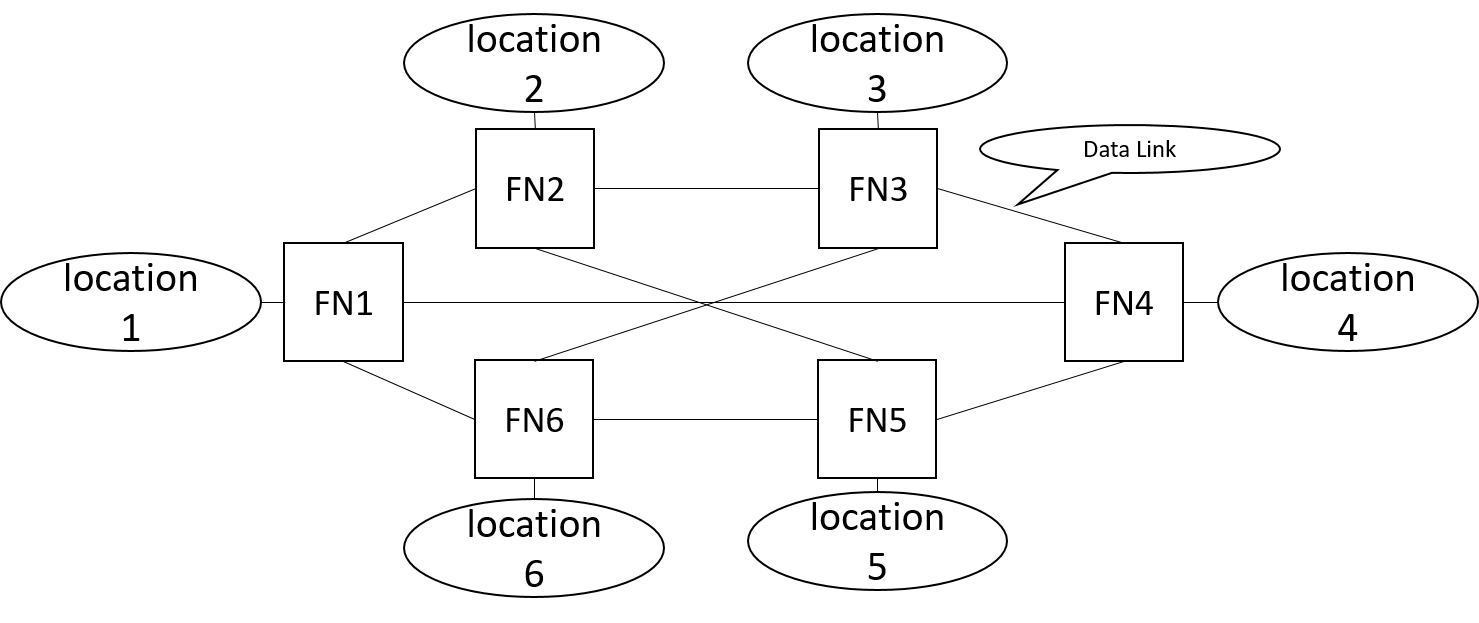
\includegraphics[width=1.0\textwidth]{./Figures/system_topology_allConnected.png}
    \caption{\label{fig: all connected topology}The (almost all connected) topology of the fog computing system.}
\end{figure}

\begin{figure}
    \centering
    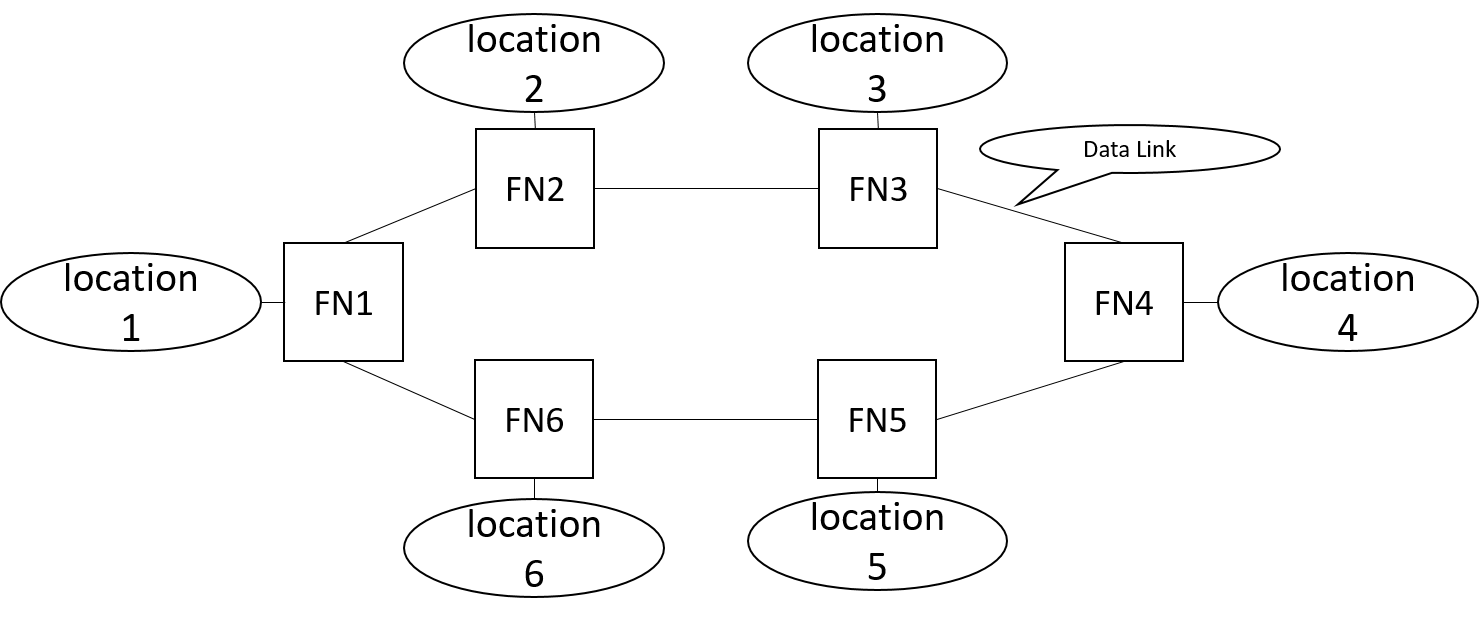
\includegraphics[width=1.0\textwidth]{./Figures/system_topology_ring.png}
    \caption{\label{fig: ring topology}The (ring) topology of the fog computing system.}
\end{figure}

\begin{figure}
    \centering
    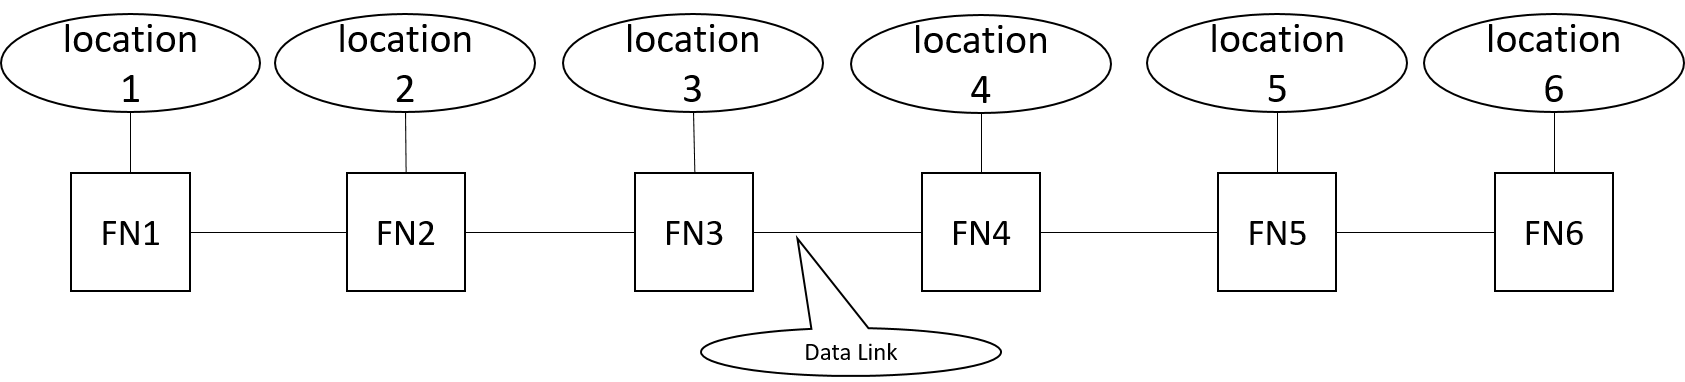
\includegraphics[width=1.0\textwidth]{./Figures/system_topology_line.png}
    \caption{\label{fig: line topology}The (line) topology of the fog computing system.}
\end{figure}

The number of tasks in this time period is $|I| = 40$. The arrival time $T_i^a$ follows a continuous uniform distribution $ U(0, 10) $, so that no tasks arrive at exactly the same time, which is an assumption we made earlier in our RAFC model. Moreover, the number of endpoints for each task $E_i$ is generated uniformly from $ \{ 1,2,\ldots,6 \} $, and the location of each endpoint $u_{e,l}^i$ is chosen uniformly at random from all locations $L$ with replacement.

Furthermore, we choose a special valuation function $ v_i $ in our simulations for simplicity, which is a non-decreasing linear function of the actual usage time $ \tilde{t}_i $:
\[ v_i(\tilde{t}_i) =
\begin{cases}
g_i \times \tilde{t}_i & \text{if} \; \tilde{t}_i \leq t_i  \\
g_i \times t_i  &    \text{if} \; \tilde{t}_i > t_i
\end{cases} 
\]
where the valuation coefficient $g_i$ represents task $ i $'s obtained value per usage time. 
An example of such a valuation function is shown in Figure \ref{fig:function}. 
\begin{figure}
    \centering
    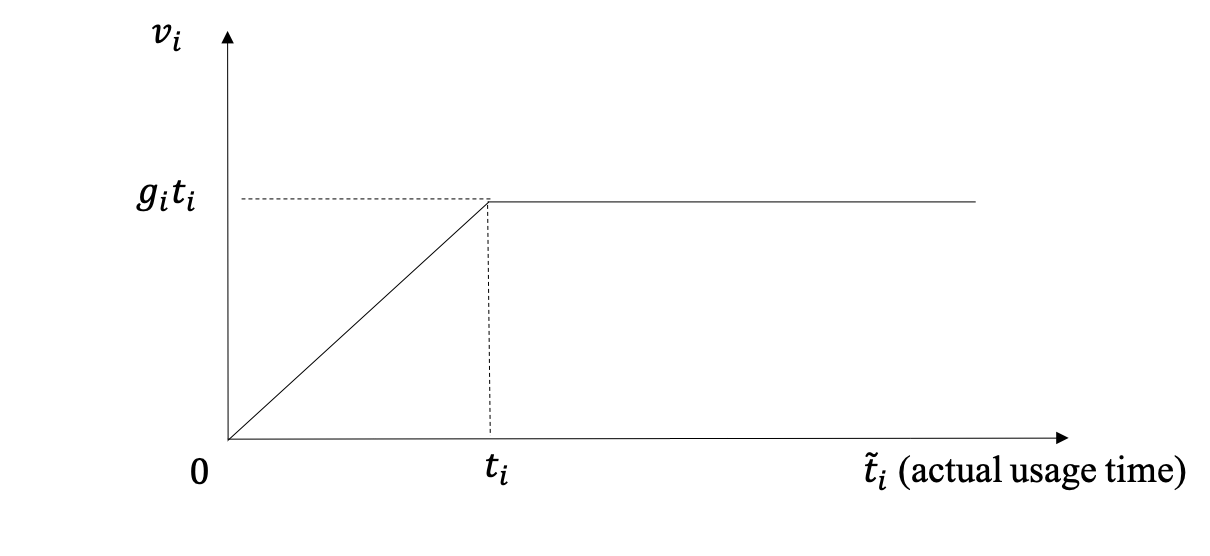
\includegraphics[width=0.8\textwidth]{./Figures/valuation_function.png}
    \caption{\label{fig:function} The valuation function of task $i$.}
\end{figure}

To make the resource allocation more realistic, there are two types of tasks in this synthetic data: low-value tasks and high-value tasks. The proportion of high-value tasks is denoted as $ q \in [0, 1] $. For task $ i $ of either type: $a_{i,r} \; \forall r \in R$ and $\Gamma_l^i \; \forall l \in L$ are all generated from a Gaussian distribution $\mathcal{N} (1, 1)$ with negative results discarded. The usage duration $t_i$ is a positive integer uniformly chosen from $\{ 1,2,3,4 \} $, and the start time $T_i^s$ is an integer uniformly chosen within 2 time steps after the arrival time: $\{ \lceil{T_i^a}\rceil, \lceil{T_i^a}\rceil + 1, \lceil T_i^a \rceil +2 \} $. Furthermore, the deadline $T_i^f$ is an integer uniformly chosen between $ a $ and $ b $ time steps after the earliest finish time (not exceeding the last time step): $\{ T_i^s+t_i-1+a,T_i^s+t_i+a,\ldots, min(T_i^s+t_i-1+b, |T|) \} $. So $ (a, b)$ defines the deadline slackness of the task, which is an important parameter because it reflects the task's flexibility. For a low-value task $ i $, $g_i$ is uniformly chosen from a continuous interval: $[8,30]$. However, for a high-value task $ i $,  $g_i$ is uniformly chosen from a continuous interval: $[180,200]$. Thus, the upper bound of the ratio of different valuation coefficient $ F = 200/8 = 25 $ in this case. 



Finally, the overall resource capacity of each computational resource $ r $: $\sum_{w \in W} A_{w,r}$ is set to be a $k$ fraction of the corresponding total resource demand: $\sum_{i \in I}a_{i,r}$, and the overall bandwidth capacity: $\sum_{(j, k) \in \mathbb{E}}b_{j, k}$ is set to be a $2k$ fraction of the total bandwidth demands: $\sum_{i\in I, l\in L}\Gamma_l^i$ because data traffic usually flows though multiple data links. Then, each FN receives the same fraction of resource $ r $: $ \frac{\sum_{w \in W} A_{w,r}}{|W|} $, and each data link receives the same fraction of the available total bandwidth: $ \frac{\sum_{(j, k) \in \mathbb{E}}b_{j, k}}{|\mathbb{E}|} $. Finally, the unit operational costs at different FNs and links: $o_{w,r} \, w \in W, r \in R \textrm{ and } o_{j, k}, (j, k) \in \mathbb{E}$ are all generated uniformly from [0.03, 0.1]. 

\section{Results and Analysis} \label{results and analysis}

We have tested the robustness of our mechanism by running simulations with different parameters, such as topologies of the network, resource scarcity in FNs and data links and deadline slackness of tasks. Across all of these settings, trends are similar. In particular, the FlexOG's performance in social welfare is typically around 90\% of the theoretical upper bound, and between 5-10\% better than OG's. In the following, we will show the results of these simulations and analyse them. 

\subsection{Social Welfare of Different Resource Scarcity}

\begin{figure}[h]
    \centering
    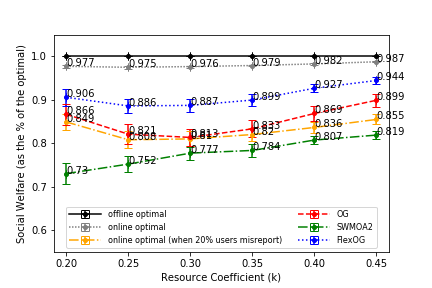
\includegraphics[width=0.8\textwidth]{./Figures/comparison of social welfare (resource-coefficient).png}
    \caption{The social welfare achieved by four mechanisms with parameters ($ (a, b) = (5, 10), F = 25, q = 0.1 $) and almost all connected network.}
    \label{fig: social_welfare_resource_coefficient} 
\end{figure}


\begin{figure}[h]
    \centering
    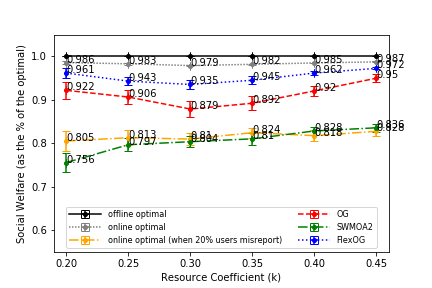
\includegraphics[width=0.8\textwidth]{./Figures/comparison of social welfare (resource-coefficient) (ring).png}
    \caption{The social welfare achieved by four mechanisms with parameters ($ (a, b) = (5, 10), F = 25, q = 0.1 $) and ring network.}
    \label{fig: social_welfare_resource_coefficient_ring} 
\end{figure}

\begin{figure}[h]
    \centering
    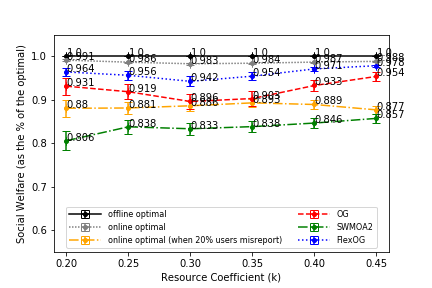
\includegraphics[width=0.8\textwidth]{./Figures/comparison of social welfare (resource-coefficient) (line).png}
    \caption{The social welfare achieved by four mechanisms with parameters ($ (a, b) = (5, 10), F = 25, q = 0.1 $) and line network.}
    \label{fig: social_welfare_resource_coefficient_line} 
\end{figure}


First, we compare the total social welfare achieved by FlexOG with other benchmarks under different resource coefficients $ k $ indicating the scarcity of the resources in Figure \ref{fig: social_welfare_resource_coefficient}, Figure \ref{fig: social_welfare_resource_coefficient_ring} and Figure \ref{fig: social_welfare_resource_coefficient_line}.\footnote{All figures are with 95\% confidence intervals based on 200 trials, and the relative tolerance of the CPLEX optimizer is set to 1\% for offline optimal, and 5 \% for other mechanisms. (A 1\% tolerance means that the optimiser stops when a solution is within 1\% of optimality) The reason we set the relative tolerance for offline optimal lower is to make the upper bound of social welfare more accurate.} Note that we normalise the results to the performance of offline optimal so that it is easier to compare the performance of different mechanisms. Since the trend of all three figures is similar, we analyse Figure \ref{fig: social_welfare_resource_coefficient} as a representative in the following. 

Figure \ref{fig: social_welfare_resource_coefficient} shows that FlexOG consistently achieves better social welfare than other truthful benchmark mechanisms (i.e., OG and SWMOA2). In particular, SWMOA2 always has the worst performance mainly because its virtual prices are exponential to the load factors of resource, and this hinders tasks from getting allocated even when there is enough resource for them. This phenomenon gets even more significant when the resource is more scarce. For example, the average social welfare achieved by SWMOA2 is only 78.15\% of that achieved by FlexOG when the resource coefficient $ k = 0.2 $, while for other higher $ k $ this number is around 87\%. This is because, with a scarcer resource, the load factors of resource increase faster, and so is the virtual prices.

%It is worth noting that, although the price function of SWMOA can guarantee that the allocation will not break the resource constraints for the problem model in~\cite{shi2017online}, it no longer has this function in our model.
Furthermore, the performance of FlexOG is about 5\%-10\% better than that of OG in terms of social welfare. The reason for this is that under FlexOG when and how committed time steps are allocated to tasks is flexible. Therefore, FlexOG can reschedule unfinished tasks to allocate more time steps for the newly arrived high-value task, while OG cannot do this. The Figure also shows that the performance difference between FlexOG and OG shrinks when the resource coefficient $ k $ is either very small or very big. Intuitively, this is because when there are few resources or there are abundant resources the performance of OG will be closer to the optimal, and there is less space for FlexOG to improve social welfare by rescheduling tasks. This indicates that the superiority of FlexOG is more significant when resources are neither too scarce nor too abundant, which is in correspondence with reality in most cases.

In addition, our mechanism also performs close to offline optimal, achieving around $ 90\% $, which indicates that our mechanism is efficient even though it is online. Interestingly, the performance of online optimal is very close to that of offline optimal. The main reason is that all tasks are preemptible, so myopic decisions will not have a big effect in the future. If a high-value task arrives, online optimal can always pause some low-value tasks to process the newly arrived high-value one. However, online optimal is not truthful and vulnerable to manipulations. So, although online optimal performs about 10\% better than FlexOG, its performance drops below that of FlexOG when just 20\% of users misreport. Here, users who misreport only misreport their valuation coefficient much higher (as 1 million), and report other information truthfully. So the performance of online optimal is mainly used as an indicator of the upper bound of online resource allocation here. In addition, we have also tested whether users have the incentive to misreport by comparing utilities of truthful and non-truthful users (see Section \ref{utility evaluation}), and the result shows on average non-truthful users get a higher utility. This means that, in a strategic setting where users can misreport, FlexOG can actually achieve significantly more social welfare than online optimal. 

%may write something more about this phenomenon 

\begin{figure}[h]
    \centering
    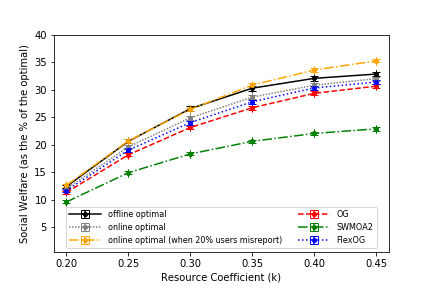
\includegraphics[width=0.8\textwidth]{./Figures/comparison of accepted number (resource-coefficient).png}
    \caption{The number of tasks got allocated by four mechanisms with parameters ($ (a, b) = (5, 10), F = 25, q = 0.1 $) and all connected network.}
    \label{fig: accepted_number_resource_coefficient} 
\end{figure}

Finally, Figure \ref{fig: accepted_number_resource_coefficient} shows the number of tasks that get allocated (i.e., get at least one time step usage time) under different mechanisms with almost all connected network. The result is similar for other network topologies, so their results are omitted in this thesis. We can see from the figure that resources are truly scarce when $ k= 0.2 $ because only around 30\% of tasks get allocated under offline optimal. While the resources are relatively abundant when $ k = 0.45 $, where around 75\% of tasks get allocated under offline optimal. In addition, FlexOG only allocates about one or two tasks more than OG on average, which means that FlexOG achieves more social welfare mainly by giving more usage time to high-value tasks rather than getting more tasks allocated. Interestingly, more tasks get allocated under online optimal when 20\% of users misreport than offline optimal. Intuitively, this is because some low-value tasks which will not get allocated under other mechanisms can get some usage time by misreporting high valuations. Besides, since the virtual cost of SWMOA2 is often much higher than the operational cost and prevent tasks from getting allocated even when there is enough resource to process them, it has the lowest number of allocated tasks. 


%\begin{figure}[h]
%    \centering
%    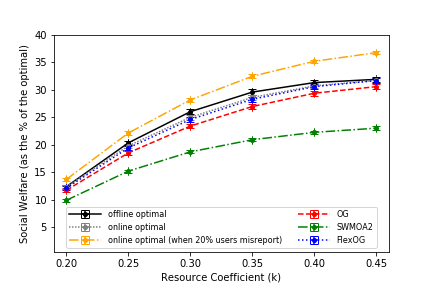
\includegraphics[width=0.8\textwidth]{./Figures/comparison of accepted number (resource-coefficient) (ring).png}
%    \caption{The social welfare achieved by four mechanisms with parameters ($ (a, b) = (5, 10), F = 25, q = 0.1 $) and ring network.}
%    \label{fig: accepted_number_resource_coefficient_ring} 
%\end{figure}
%
%\begin{figure}[h]
%    \centering
%    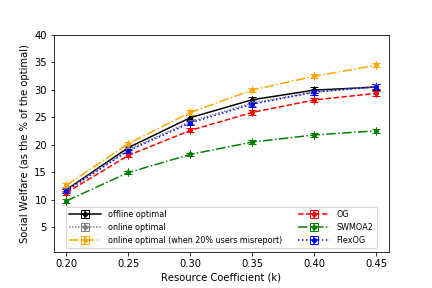
\includegraphics[width=0.8\textwidth]{./Figures/comparison of accepted number (resource-coefficient) (line).png}
%    \caption{The social welfare achieved by four mechanisms with parameters ($ (a, b) = (5, 10), F = 25, q = 0.1 $) and line network.}
%    \label{fig: accepted_number_resource_coefficient_line} 
%\end{figure}

%
%The main reason that SWMOA2 performed the worst is that the virtual resource costs increase exponentially as more resources are being occupied so that some tasks are rejected even when there are still enough resources to run them. The flexible online greedy mechanism performs better than online greedy because it has more flexibility for resource allocation and can dynamically adjust its resource allocation scheme as new tasks are being submitted. 



\subsection{Social Welfare of Different Deadline Slackness}

Next, we compare the performance in social welfare under different levels of deadline slackness in various network topologies (Figure \ref{fig: social_welfare_deadline_slackeness}, \ref{fig: social_welfare_deadline_slackeness_ring} and \ref{fig: social_welfare_deadline_slackeness_line}). A task with a bigger deadline slackness has more time steps between its earliest possible finish time and its deadlines and is more flexible to allocate. As can be seen from the figures, the gap between FlexOG and OG increases as the deadline slackness of tasks increases. This is because when tasks are more flexible, FlexOG is more likely to reschedule low-value tasks to allocate more high-value tasks, while OG cannot benefit from this since its resource allocation is fixed once it has been made. In addition, SWMOA2's performance is quite stable in terms of different deadline slackness. This is because, instead of the flexibility of tasks, the virtual prices of resource play a major role in affecting the performance of SWMOA2.

\begin{figure}[h]
    \centering
    \includegraphics[width=0.8\textwidth]{./Figures/"comparison of social welfare (slackness)".png}
    \caption{The social welfare achieved by four mechanisms with parameters ($ (a, b) = \{ (0, 5), (1, 6), (2,7) (3, 8),(4, 9), (5, 10) \}, F=25, q=0.1, k=0.3 $) and all connected network.}
    \label{fig: social_welfare_deadline_slackeness}
\end{figure}

\begin{figure}[h]
    \centering
    \includegraphics[width=0.8\textwidth]{./Figures/"comparison of social welfare (slackness) (ring)".png}
    \caption{The social welfare achieved by four mechanisms with parameters ($ (a, b) = \{ (0, 5), (1, 6), (2,7) (3, 8),(4, 9), (5, 10) \}, F=25, q=0.1, k=0.3 $) and ring network.}
    \label{fig: social_welfare_deadline_slackeness_ring}
\end{figure}

\begin{figure}[h]
    \centering
    \includegraphics[width=0.8\textwidth]{./Figures/"comparison of social welfare (slackness) (line)".png}
    \caption{The social welfare achieved by four mechanisms with parameters ($ (a, b) = \{ (0, 5), (1, 6), (2,7) (3, 8),(4, 9), (5, 10) \}, F=25, q=0.1, k=0.3 $) and line network.}
    \label{fig: social_welfare_deadline_slackeness_line}
\end{figure}

\subsection{Processing Time of Different Mechanisms}

\begin{figure}
    \centering
    \includegraphics[width=1.0\textwidth]{./Figures/"comparison of processing time (resource-coefficient)".png}
    \caption{The processing time of four mechanisms with parameters ($ (a, b) = (5, 10), F = 25, q = 0.1 $) and all connected network.}
    \label{fig: processing time}
\end{figure}

\begin{figure}
    \centering
    \includegraphics[width=1.0\textwidth]{./Figures/"comparison of processing time (resource-coefficient) (ring)".png}
    \caption{The processing time of four mechanisms with parameters ($ (a, b) = (5, 10), F = 25, q = 0.1 $) and ring network.}
    \label{fig: processing time_ring}
\end{figure}

\begin{figure}
    \centering
    \includegraphics[width=1.0\textwidth]{./Figures/"comparison of processing time (resource-coefficient) (line)".png}
    \caption{The processing time of four mechanisms with parameters ($ (a, b) = (5, 10), F = 25, q = 0.1 $) and line network.}
    \label{fig: processing time_line}
\end{figure}

In this section, we compare the processing time of FlexOG with the benchmark mechanisms. The processing time is also important because many users cannot wait for a long time for an allocation decision, and the fog provider does not want to use too much computing resource on making allocation decisions. Thus, in this thesis, the shorter the processing time, the better (Challenge \ref{itm: Challenge scalability}). Now, the simulation was conducted on the Iridis 4 Compute Cluster~\footnote{https://hpc.soton.ac.uk/redmine/projects/iridis-4-support/wiki}, using four cores of an Intel Xeon E5-2670 (`Sandybridge') processor with 16GB RAM. 

The results are shown in Figure \ref{fig: processing time}, Figure \ref{fig: processing time_ring} and Figure \ref{fig: processing time_line}. We plot the processing time of all mechanisms under resource coefficients $ k = 0.25 $, $ k = 0.35 $ and $k = 0.45 $. The processing time under other resource coefficients has a similar trend and is not plotted to make the figures easier to read. Note that the boxes show the lower to upper 25\% values of the data with whiskers showing 5 to 95 percentile of the data, and the outliers are discarded. 

The figure shows that on average, offline optimal takes the least processing time, online optimal and OG take more processing time, and SWMOA2 and FlexOG uses the most processing time. This is mainly because offline optimal only needs to solve the optimisation problem once, while all other mechanisms need to solve the optimisation problem multiple times. Online optimal needs to solve the optimisation problem at the start of each time step, so it needs to solve it $ |T| - 1 = 11 $ times. The remaining mechanisms all need to solve the optimisation problem when a new task arrives, so they need to solve it $ |I| = 40 $ times. However, the processing time of offline optimal is much more than $ \frac{1}{11} $ of that of online optimal. This is because offline optimal need to make a resource allocation decision for all tasks at once, while online optimal only need to make a decision for tasks arrived in the previous time step every time. So offline optimal's optimisation problems have more decision variables and take more time to solve on average. Another reason is that the relative tolerance of offline optimal is set to be $ 0.01 $ while this parameter is set $ 0.05 $ for other mechanisms, which also makes offline optimal takes more time to find a solution to its optimisation problem.

Similarly, although OG needs to solve the optimisation problem four times as many as online optimal, they have similar processing time on average. This is because OG only needs to make a resource allocation decision for just one task at a time. So, its optimisation problem solves faster than online optimal's on average. 

Finally, FlexOG takes the most time because it not only needs to solve the optimisation problem $ |I| = 40 $ times, but its optimisation problems also have more decision variables. This is because it needs to make allocation decisions for all flexible tasks each time a new task arrives. The reason why SWMOA2 takes second-most time on average is that SWMOA2 needs to compute the load factor and virtual price of each resource after every allocation decision, while other mechanisms just use the fixed operational cost of each resource. Interestingly, the processing time of FlexOG also has a wider dispersion than other mechanisms. This is because with more optimisation problems to solve and with more decision variables, FlexOG has more probability of coming across optimisation problems that are hard to solve. For each task, FlexOG takes around four seconds to make the allocation decision on average. For tasks whose arrival time is much earlier than their start time, it is feasible to use FlexOG because there is sufficient time for FlexOG to make allocation decisions. However, if the arrival time and the start time of a task are the same, or tasks arrive frequently, then the processing time of FlexOG will become an issue. We will discuss how we plan to solve this issue in the future work section (Section \ref{future work}).


\subsection{Utility of Truthful and Non-truthful Users} \label{utility evaluation}

\begin{figure}
    \centering
    \includegraphics[width=0.8\textwidth]{./Figures/"comparison of social welfare (misreport)".png}
    \caption{Utility comparison between truthful and non-truthful users ($ (a, b) = (5, 10), F = 25, q = 0.1 $) in all connected network.}
    \label{fig: utility misreport}
\end{figure}

In this section, we discuss whether fog users are incentivised to report their tasks truthfully by comparing average utilities of truthful and non-truthful users. The result of how much percentage of the whole tasks value they can get for all fog users, truthful users and non-truthful users respectively under the online optimal mechanism in the almost all connected topology is shown in Figure \ref{fig: utility misreport}. Recall that non-truthful users only misreport their valuation coefficient as one million. This is because if they can have advantages in utilities over truthful users by misreporting their valuation coefficient, they will have even bigger advantages when they misreport other information as well. The figure shows that non-truthful users have similar utility as truthful users when 20\% of fog users are non-truthful. However, the utilities of truthful users decrease rapidly as more users become non-truthful, and non-truthful users have about 67\% more utilities than truthful users on average when 80\% of users are non-truthful. This is because the reported valuation coefficients of non-truthful users are much higher than that of truthful users. Online optimal will always prioritise non-truthful users when it makes allocation decisions. This means that under online optimal, fog users have no incentives to be truthful. The social welfare achieved by online optimal when all users report their types truthfully cannot be achieved in a strategic setting.

Figure \ref{fig: utility misreport} also indicates that non-truthful users have a negative impact on the overall utility (social welfare). This is due to the fact that online optimal makes allocation decisions based on false valuation coefficients, so it may priorities a low-value task over a high-value task. However, when all users are non-truthful, online optimal achieves a slightly higher social welfare than that when 80\% users are non-truthful. The reason for this is that when all users are non-truthful, their valuation coefficients are all one million, the case where a low-value task is priorities over a high-value task because of its misreported valuation coefficient disappears. The reason why social welfare is lower when all users are non-truthful than that when all users are truthful is mainly that low-value tasks are still prioritised because they need fewer resources on average.




\section{Summary}
In this chapter, we described the synthetic data used in our simulations and analysed the results from a number of empirical simulations. These results highlighted the advantages of the FlexOG mechanism, which consistently outperformed all truthful benchmarks and achieved a social welfare near the theoretical upper bound. Furthermore, we also showed that fog users are incentivised to misreport their types under the non-truthful benchmark online optimal, which degrades social welfare significantly. Specifically, online optimal is outperformed by FlexOG when only 20\% of fog users misreport. Besides, the results showed that the advantage of FlexOG is bigger when resources are neither scarce nor sufficient and when tasks have more deadline slackness, which is common in practice. Therefore, our proposed mechanism FlexOG addresses the high social welfare resource allocation challenge (Challenge \ref{itm: Challenge social welfare}). Nevertheless, simulations showed that it usually takes around 2-6 seconds for FlexOG to make an allocation decision for a newly arrived task. Although this is fine to tasks with a long time between their arrival times and start times, it is infeasible to tasks whose arrival times equal or are close to their start times or tasks that arrive frequently. So the timely resource allocation challenge (Challenge \ref{itm: Challenge scalability}) has only been partly addressed. We will discuss this in detail in the future work section (Section \ref{future work}).

\chapter{Conclusions and Future Work} \label{conclusions and future work}

The final chapter concludes this thesis by reviewing its contributions to the field of RAFC and by outlining possible directions for future work. To this end, in Section \ref{research summary}, we cast our mind back at the motivations of this thesis and provide a general overview of the techniques we have proposed to deal with it. Then, in Section \ref{research contributions}, we describe our research contributions in detail and relate them back to our research challenges from Section \ref{challenges}, and in Section \ref{empirical evaluation of FlexOG}, we summarise the evaluation results of our proposed mechanism by comparing it with benchmarks. Finally, in Section \ref{future work}, we propose several possible ways in which our mechanism can be extended in the future.

\section{Research Summary} \label{research summary}

Nowadays, the IoT is developing very fast and is predicted to revolutionise the way we work and live by making all kinds of physical devices into IoT devices and connect them to the Internet. In this context, fog computing is proposed to complement cloud computing in providing computing resource to IoT devices. Fog computing has many important benefits, such as low latency and reducing data traffic, which are critical to the popularisation of the IoT. 

Hitherto there is no truthful resource allocation mechanism that achieves high social welfare in our RAFC model. As we have argued in this thesis, it is necessary to treat fog users as intelligent agents who are rational and have their own goals (i.e., utility maximisation). Therefore, it is vital to make sure the resource allocation mechanism is truthful and thus can be used in strategic settings. 

Reviewing the existing resource allocation mechanisms, we found that they cannot apply to our RAFC model or only address part of our research challenges. A lot of existing approaches only deal with homogeneous resource allocation, whereas there are several heterogeneous resources in RAFC. Some other approaches can only be used in offline settings, while in RAFC tasks arrive over time and allocation decisions must be made upon tasks arrival without future information. Finally, most existing mechanisms are not truthful and infeasible to work in strategic settings. 

In the following section, we provide a summary of our mechanism, including the contributions we have made to the state of the art and how it addresses the research challenges listed in Section \ref{challenges}. 

\section{Research Contributions} \label{research contributions}

In this thesis, we aimed to design a truthful resource allocation mechanism for our RAFC problem that is efficient in terms of social welfare. We achieved this by extending a class of mechanisms called price-based mechanisms and a technique called pre-commitment. In the following, we outline each of the contributions of this thesis along with the research challenges they address (Section \ref{formulation of the RAFC problem}-\ref{design of FlexOG}). 

\subsection{Formulation of the RAFC Problem} \label{formulation of the RAFC problem}

In this thesis, we described the RAFC problem we study in detail and formulated it as a constraint optimisation problem (Optimisation Problem \ref{eq: constraint_optimisation_problem}) considering all related research challenges (Challenges \ref{itm: Challenge bandwidth}, \ref{itm: Challenge VM}, \ref{itm: Challenge time-oriented}, \ref{itm: Challenge social welfare} and \ref{itm: Challenge cost-aware}). Firstly, the optimisation problem including the bandwidth and traffic routing constraints (Challenge \ref{itm: Challenge bandwidth}). Secondly, it allows dynamic generation of VMs in any FNs (Challenge \ref{itm: Challenge VM}) and uses time-oriented valuation functions (Challenge \ref{itm: Challenge time-oriented}). Finally, its objective function includes the operational cost of the fog (Challenge \ref{itm: Challenge cost-aware}) and is to maximise the social welfare (Challenge \ref{itm: Challenge social welfare}). 

\subsection{Design of FlexOG} \label{design of FlexOG}

In order to allocate resources efficiently in strategic settings (challenge \ref{itm: Challenge social welfare}, \ref{itm: Challenge online} and \ref{itm: Challenge truthful}), we designed a price-based online mechanism called FlexOG. This mechanism belongs to a class of mechanisms called price-based mechanisms, which ensures that it is truthful and works in strategic settings. Furthermore, FlexOG uses a technique called pre-commitment, which means that FlexOG only commits the usage time to a task when it arrives but leaves how the usage time is scheduled flexible. This technique gives FlexOG an advantage in achieving higher social welfare than benchmark mechanisms. 

\section{Empirical Evaluation of FlexOG} \label{empirical evaluation of FlexOG}

To make sure that FlexOG can truly achieve higher social welfare than other state-of-the-art mechanisms (Challenge \ref{itm: Challenge social welfare}), we did extensive simulations to evaluate the performance of FlexOG. More specifically, we evaluate FlexOG using synthetic data of different network topologies, resource scarcities or deadline slackness of tasks. Across all of these settings, FlexOG achieves social welfare higher than the two truthful benchmarks (around 5-10\% better than OG, and 10-20\% better than SWMOA2) and close to the theoretical upper bound (around 90\%). In particular, we showed through simulations that users are incentivised to misreport under the non-truthful benchmark online optimal, and the social welfare achieve by online optimal falls below FlexOG when 20\% of users misreport their valuation. In short, these simulations indicated that FlexOG outperforms all benchmarks in strategic settings. 


%In this report, we introduced the concept of fog computing and the model of its resource allocation. We analysed why it is meaningful to do this research and the research challenges we may need to deal with. Unlike resource allocation for cloud computing, we need to consider where to place the VM and how to allocate bandwidth in resource allocation for fog computing. 
%
%Furthermore, we have investigated some related work on resource allocation. Some of them are not truthful, and others that use mechanism design theory are truthful. Additionally, some basic concepts and theorems of mechanism design are outlined too. They are the basis of our work. In conclusion, the existing literature is either not specifically dealing with the fog computing resource allocation or using a less practical resource allocation model. 
%
%In chapter 3, we described our model of fog computing resource allocation and presented our proposed mechanism for this model. Our goal is to design a social welfare efficient mechanism for our fog computing resource allocation model. Simulations show that our mechanism performs better than other truthful benchmark mechanisms in social welfare. This mechanism will be the basis of our future work.


\section{Future Work} \label{future work}

The work in this thesis can be extended in various ways. First, we plan to complement the empirical evaluation of resource allocation mechanisms with real data evaluation or using fog computing simulation tools, and we detail these in Section \ref{future empirical evaluation}. Second, we aim to design mechanisms which are more scalable or more efficient in social welfare. We discuss how these might be done in Section \ref{future resource allocation mechanisms}. Finally, we draw a Gantt chart of the future work plan.

\subsection{Future Empirical Evaluation} \label{future empirical evaluation}

Although our evaluation is performed over a variety of configurations of the synthetic data, it is still of value to evaluate FlexOG using real data. Although, there lacks comprehensive real-world data from fog computing systems, one way to circumvent this problem is to combining real-world cloud computing data with synthetic data. For example, we can set the amount of resources required by a VM according to the resource demand of each task in Google cluster data and generate other data such as the number of IoT devices, bandwidth demands and required usage time of each tasks synthetically. Some work takes this approach to evaluate their mechanisms~\citep{zhang2015truthful,shi2017online}. 

Another way to make the evaluation more convincing is to use widely accepted simulation tools for fog computing such as \textit{FogNetSim++}~\citep{qayyum2018fognetsim++} and \textit{iFogSim}~\citep{gupta2017ifogsim}. They enables simulations of fog computing environments for evaluating resource allocation mechanisms. There is much work used such tools to evaluate their approaches, especially \textit{iFogSim}\citep{rahbari2017scheduling,taneja2017resource}. Thus, to extend our empirical evaluation, we can either adapt available cloud computing data to our RAFC model or use a widely accepted simulation tool for fog computing in future work. 


\subsection{Future Resource Allocation Mechanisms} \label{future resource allocation mechanisms}

\begin{enumerate}
	\item We plan to improve the scalability of our mechanism. Our simulations showed that the mechanism we proposed in this report-FlexOG needs
	$ 4-5 $ seconds on average to make an allocation decision for a newly arrived task. Furthermore, our simulations are only on a small setting with 6 FNs, 6 locations, 12 time steps and 40 tasks. In reality, fog computing system can have thousands of FNs and tasks. Therefore, the scalability of FlexOG needs to be improved to make it more practical. One approach to improve the scalability is to simplify the associated data routing problem. For example, we could restrict the number of hops from IoT devices of a task to the VM of that task, which is also in accordance with the low latency requirements of IoT applications. Another option is to design an efficient algorithm to solve the MILP problem of social welfare maximisation instead of solving it using CPLEX. Finally, we are also considering to use sub-optimal heuristics, for example by greedily allocating tasks based on their value densities. Since finding the optimal allocation for newly-arrived tasks is critical to the truthfulness of FlexOG, we would need to ensure that the DSIC and IR properties still hold. Thus, using heuristics instead of solving the optimisation problem is challenging.
	
	\item To design mechanisms that are more efficient in social welfare, we are considering using online auctions or reinforcement learning techniques instead of price-based mechanisms to allocate resources. Under online auction mechanisms, resource allocation decisions are made at the start of each time step instead of at the arrival of new tasks. Therefore, decisions are based on more information and can achieve higher social welfare. However, intuitively, users may get more utility by reporting their tasks within a time step that are ``less competitive'', which means that during that time step only few high-value tasks are reported. Thus, the online auction mechanisms need to be carefully designed to be truthful. Another approach to design a truthful mechanism that is more efficient in terms of social welfare is to combine mechanism design and reinforcement learning techniques. In reality, the external environment can be dynamic, and the pattern of IoT tasks can gradually change over time. For example, the percentage of high-value tasks may be much higher this week than last week. This approach is promising since mechanisms designed using this approach can achieve higher social welfare by automatically adjusting to dynamic environments. For example, there are researches showing that reinforcement learning approach can achieve high efficacy in a dynamic environment~\citep{aydin2000dynamic,cui2017reinforcement}. However, users may misreport tasks to increase their utility immediately or to influence what the mechanism learn and gain advantage in the future. So the mechanism needs to ensure that any users cannot be better off at present or in the future by misreporting their tasks. For this reason, we also need to carefully design the reinforcement learning mechanism to make it truthful and efficient at the same time. 
	
	
\end{enumerate}

The following figure is a rough work plan for the next 15 months until the PhD thesis.

\begin{sidewaysfigure}[h]
	\center
	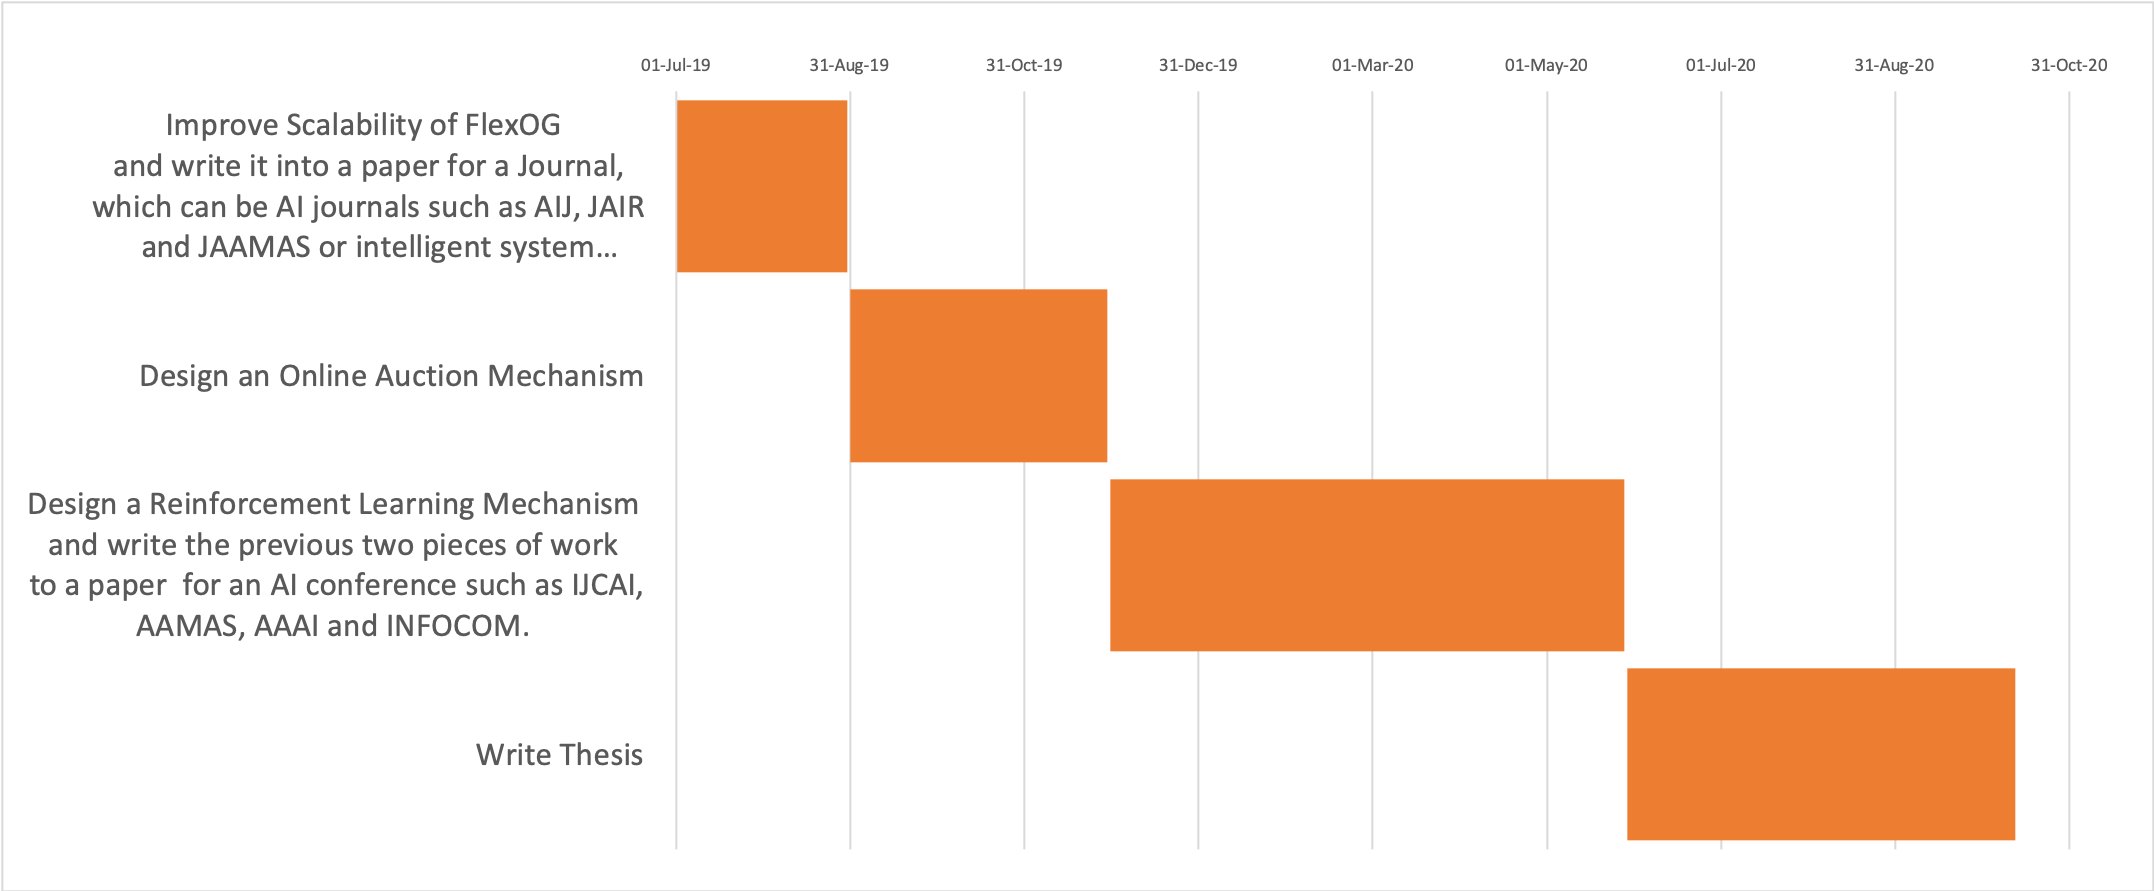
\includegraphics[width = 1\textwidth]{./Figures/GanttChart.png}
	\caption{Gantt chart up to PhD thesis}
	\label{fig:Gantt chart}
	%   \source{\citep{evans2011internet}}
\end{sidewaysfigure}


\appendix
\chapter{Appendix}
The text for an appendix goes here.

%% ----------------------------------------------------------------
\backmatter
\bibliographystyle{named}
\bibliography{thesis}
\end{document}
%% ----------------------------------------------------------------
